\documentclass[12pt]{article}
\usepackage[utf8]{inputenc}
\usepackage{graphicx}
\usepackage[bahasa]{babel}
\usepackage{amsfonts, amsmath, amssymb, mathtools, enumitem}
\usepackage{geometry}
\usepackage{hyperref}
\usepackage{appendix}
\usepackage{lmodern}
\usepackage{tikz}
\usetikzlibrary{shapes.geometric, arrows}
\tikzstyle{startstop} = [rectangle, rounded corners, minimum width=3cm, minimum height=1cm,text centered, draw=black, fill=blue!15]
\tikzstyle{arrow} = [thick,->,>=stealth]
\geometry{left=1in,right=0.75in,top=1in,bottom=1in}
\usepackage{lmodern}
\usepackage{indentfirst}
\usepackage{chngcntr}
\usepackage{listings}
\usepackage{hyperref}
\counterwithin{equation}{section}
\setlength{\parskip}{1em}

\begin{document}

\begin{titlepage}
    \begin{center}
        \vspace*{1cm}
            
        \Huge
        \textbf{Permodelan Harga Laptop dengan \textit{Generalized Linear Model} \\ AK4082}
            
        \vspace{0.5cm}
        \LARGE
        Tugas Besar

            
        \vspace{1.5cm}
        
\includegraphics[width=0.4\textwidth]{logo_itb_1024.png}
        \\
        
        \vspace{1cm}
        
        \Large
                \textbf{Kelompok 14:}\\
        Leonardo Valentino Kosasih - 10818015 \\
        Hari/Tanggal : Selasa, 18 Mei 2021
    \end{center}
\end{titlepage}
\newpage
\tableofcontents
\newpage
\listoffigures
\newpage
\section{Latar Belakang}
Dewasa ini, penggunaan gawai meningkat tajam dari tahun-tahun sebelumnya. Tentu saja hal ini disebabkan karena mudahnya untuk mendapatkan akses internet. Belum lagi karena pandemi, hampir seluruh aktivitas sehari-hari dilakukan menggunakan gawai secara daring (dalam jaring). Tentu saja hal ini mengakibatkan banyaknya terjualnya gawai-gawai khususnya laptop dengan spesifikasi dan merk tertentu. Dan tentu saja, ke depannya laptop atau gawai yang sudah dimiliki mungkin akan dijual kembali atau bahkan di-tukar-tambahkan dengan gawai yang lebih baru. Namun yang menjadi permasalahan adalah, adakah suatu cara atau formula yang dapat memudahkan penjual maupun pembeli laptop bekas untuk menentukan harga yang sesuai ?  
\par
Dilansir dari \textit{\href{https://www.statista.com/statistics/818439/global-notebook-computer-shipment-share-by-brands/}{statista.com}}, ada 6 perusahaan dengan pangsa pasar laptop yang terbesar dari tahun 2016-2020. Diantaranya adalah : HP, Lenovo, Dell, Asus, Acer dan Apple. Pada karya tulis ini, akan dibahas suatu permodelan \textit{Generalized Linear Model} untuk menentukan harga suatu laptop dengan spesifikasi khusus. Data yang diperoleh adalah data yang diunduh di situs \textit{\href{https://www.kaggle.com/ionaskel/laptop-prices}{kaggle.com}} pada tanggal 8 Mei 2021.  
\par 
Secara umum data memiliki 1300 baris dengan 12 kolom yang berisikan merk laptop, spesifikasi piranti keras laptop dan juga harga laptop tersebut dalam mata uang Euro. Data ini diunggah oleh pemiliknya 3 tahun lalu (tepatnya tahun 2018). Sehingga harga pada data jika dibandingkan dengan harga saat ini tentunya akan berbeda karena berbagai faktor salah satunya adalah inflasi. Namun hal ini tidak menjadi suatu masalah yang besar karna tujuan dari karya tulis ini adalah untuk menentukan suatu harga yang wajar untuk pembeli maupun penjual laptop bekas.  
\par   
Penulis mengucapkan terima kasih sebesar-besarnya kepada Dra. Dumaria Rulina Tampubolon, M.Sc.,Ph.D. sebagai dosen pengampu mata kuliah AK4082 Model Linear Lanjut yang telah mengajar dan juga membimbing penulis terhadap materi terkait. Tak lupa juga untuk sahabat-sahabat penulis Farrell Theodore Adriano (10118023) dan juga Mikhael Belmiro Tirta Kusuma (10118038) yang menjadi teman diskusi dan yang selalu memberikan inspirasi dan ide mengenai pengolahan data.

%Latar Belakang, termasuk motivasi dan penjelasan tentang data yang dianalisis.
\newpage
\section{Metodologi}
Metode yang akan digunakan adalah metode regresi khususnya adalah \textit{Generalized Linear Model} atau yang akan disingkat dengan GLM. Hal ini didasari karena distribusi dari respons tidak mengikuti distribusi normal melainkan suatu distribusi keluarga eksponensial yang fungsi kepadatan peluangnya dapat ditulis dalam formula : 
\begin{equation}
\label{Family_Expo}
    f(y) = c(y,\phi)\exp\left(\frac{y\theta-a(\theta)}{\phi}\right)
\end{equation}
Dengan $y$ adalah respons, $\phi$ adalah parameter dispersi, dan $\theta$ adalah parameter kanonik. 
\par 
Perbedaan yang paling mendasar antara GLM dan model regresi linear klasik adalah fungsi rataan respons yang linear terhadap parameternya. Sehingga diperoleh suatu persamaan 
\begin{equation}
    \label{ge_el_em}
    g(\mu) = \mathbf{x}'\mathbf{\beta}
\end{equation}
Dengan $g(\cdot)$ adalah fungsi \textit{link}, $\mathbf{x}$ adalah vektor dari variabel penjelas dan $\mathbf{\beta}$ adalah vektor dari parameter. Lebih lanjut, $g$ adalah fungsi yang monoton dan terdiferensialkan (seperti fungsi log atau fungsi akar). Parameter $\beta$ dan parameter $\phi$ ditaksir dengan menggunakan metode \textit{Maximum Likelihood}.
\par
Lebih jauh dengan metode \textit{Maximum Likelihood}, dari persamaan \ref{Family_Expo} dapat diperoleh :
\begin{equation}
    \label{llikekl}
    \ell(\beta,\phi) = \sum_{i=1}^n \ln{f(y_i;\beta,\phi)}=\sum_{i=1}^n \left(\ln{c(y_i,\phi)}+\frac{y_i\theta_i-a(\theta_i)}{\phi}\right)
\end{equation}
Sehingga untuk menaksir nilai $\beta$ dan $\phi$, persamaan \ref{llikekl} dapat diturunkan secara parsial terhadap masing-masing parameter. Sehingga diperoleh suatu bentuk matriks
\begin{equation}
    \label{matrisk}
    \mathbf{X}'D(y-\mu) = 0 \Longleftrightarrow \mathbf{X}'WG(y-\mu)=0
\end{equation}
Dengan $\mathbf{X}$ adalah matriks disain dengan ukuran $n\times (m+1)$ dengan $n$ adalah banyak observasi dan $m$ adalah banyak kolom. Perlu diingat bahwa kolom pertama dari matriks disain memiliki entri 1. $D$ adalah matriks diagonal dengan entri $\partial \theta_i/\partial \eta_i$ dengan $\eta_i = x_i\beta$ sehinga dapat dilihat bahwa 
\begin{equation}
    \label{nguli}
    \left(\frac{\partial \theta_i}{\partial \eta_i}\right)^{-1} = \frac{\partial \eta_i}{\partial \theta_i} = \frac{\partial \eta_i}{\partial \mu_i}\frac{\partial \mu_i}{\partial \theta_i} = \dot{g}(\mu_i)\ddot{a}(\theta_i)=\dot{g}(\mu_i)V(\mu_i)
\end{equation}
Sehingga dapat dilihat bahwa $D$ memiliki entri $[\dot{g}(\mu_i)V(\mu_i)]^{-1}$
sedangkan $G$ dan $W$ adalah matriks diagonal dengan entri $\dot{g}(\mu_i)$ dan $[(\dot{g}(\mu_i))^2V(\mu_i)]^{-1}$  secara beturut. 
\par
Karna parameter yang diperoleh berupa taksiran maka akan dibangun suatu selang kepercayaan dengan taraf signifikansi ($\alpha$) sebesar 5\%. Selang kepercayan tersebut didefinisikan sebagai
\begin{equation}
    g(\mu) = \mathbf{x}'\mathbf{\hat{\beta}}\pm z_{\alpha}\sqrt{\phi \mathbf{x}' \left(\mathbf{X}'W\mathbf{X}\right)\mathbf{x}}
\end{equation}
\par 
Tiap parameter $\beta$ nantinya akan diuji dengan statistik uji $\chi^2$ hanya saja dengan menggunakan bantuan piranti lunak R akan dibandingkan antara nilai $p-\text{value}$ dengan statistik uji-$t$.   
\par 
Untuk mengetahui apakah model yang diperoleh cocok dengan data maka akan dibandingkan antara \textit{saturated model} (yang dinotasikan dengan $\check{\ell}$)dengan model yang akan digunakan (yang dinotasikan dengan $\hat{\ell}$). Formulasi matematikanya adalah 
\begin{equation}
    \label{Deviance_1}
    \Delta \equiv 2(\check{\ell}-\hat{\ell}) = 2\sum_{i=1}^n\left(\frac{(y_i(\check{\theta}_i-\hat{\theta}_i- a(\check{\theta}_i)+a(\hat{\theta}_i))}{\phi}\right)
\end{equation}
Diharapkan nilai $\hat{\ell}$ dekat dengan $\check{\ell}$ yang mengindikasikan bahwa model yang dimiliki memiliki kecocokkan yang baik dengan data.
\par
Galat atau residu dari GLM berbeda dengan galat dari model regresi linear klasik karena galat dari GLM tidak berdistribusi normal dan juga tidak memiliki variansi yang konstan. Pada pembahasan kali ini, galat model akan ditinjau dalam bentuk \textit{deviance residuals} yang memiliki persamaan yang sama dengan persamaan \ref{Deviance_1} hanya saja $\Delta$ ditulis menjadi $\delta^2_i$ sehingga diperoleh sebagai berikut:
\begin{equation}
    \label{deviance}
    \delta^2_i \equiv \frac{2(y_i(\check{\theta}_i-\hat{\theta}_i- a(\check{\theta}_i)+a(\hat{\theta}_i))} {\phi}
\end{equation}
Dengan $\dot{a}(\check{\theta}_i) = y_i$ dan $g(\dot{a}(\hat{\theta}_i)) = x_i'\hat{\beta}$. Jika model yang digunakan sudah tepat dan $n$ besar maka dapat diaproksimasi dengan $\chi^2_{n-p}$ dengan $p$ adalah banyak parameter. Sehingga jika diperoleh $|\delta_i|>1$ dapat menjadi indikasi model yang digunakan kurang cocok dengan data. 
\par 
Karena pada permodelan kali ini akan digunakan 2 buah distribusi yaitu distribusi \textit{Gamma} dan distribusi \textit{Inverse Gaussian} akan dibahas secara singkat bentuk persamaannya
\subsection{Distribusi \textit{Gamma}}
Perhatikan bahwa fungsi kepadatan peluang dari distribusi \textit{Gamma} adalah : 
\begin{equation}
    \label{Gamma_chan}
    f(y) = \frac{y^{-1}}{\Gamma(\nu)}\left(\frac{y\nu}{\mu}\right)^\nu e^{-\frac{y\nu}{\mu}}, \quad y>0
\end{equation}
Dengan $E[Y] = \mu$ dan $Var(Y) = \frac{\mu^2}{\nu}$. Perhatikan bahwa persamaan \ref{Gamma_chan} dapat ditulis ulang menjadi bentuk pada persamaan \ref{ge_el_em} yaitu : 
\begin{equation}
     f(y) = \frac{y^{\nu-1}}{\Gamma(\nu)} e^{-\frac{y}{\nu^{-1}\mu} + \frac{\ln{\nu}}{\nu^{-1}} -\frac{\ln{\mu}}{\nu^{-1}}}, \quad y>0
\end{equation}
Sehingga diperoleh $\theta = -\frac{1}{\mu}$, $a(\theta) = -\ln{-\theta}$ dan $\phi =\frac{1}{\nu} $, dan \textit{deviance}-nya adalah
\begin{equation}
    \label{deviance_gamma}
    \delta_i^2 = 2\nu\sum_{i=1}^n\left(-\ln{\frac{y_i}{\hat{\mu}_i}}+\frac{y_i-\hat{\mu_i}}{\hat{\mu_i}}\right)
\end{equation}
Meskipun \textit{canonical link} dari distribusi \textit{Gamma} adalah $\mu^{-1}$, pada komputasinya jauh lebih mudah menggunakan \textit{canonical link} log.
%%%%%%%%%%%
\subsection{Distribusi \textit{Inverse Gaussian}}
Perhatikan bahwa fungsi kepadatan peluang dari distribusi \textit{Inverse Gaussian} adalah : 
\begin{equation}
    \label{inverse_gauss}
    f(y) = \frac{1}{\sqrt{2\pi y^3\sigma^2}}\exp\left(-\frac{1}{2y} \left(\frac{y-\mu}{\mu\sigma}\right)^2 \right), \quad y>0
\end{equation}
Dengan $E[Y] = \mu$ dan $Var(Y) = \sigma^2 \mu^3$. Perhatikan bahwa persamaan \ref{inverse_gauss} dapat ditulis ulang menjadi bentuk pada persamaan \ref{ge_el_em} yaitu :
\begin{equation}
    \label{inverse_gauss2}
    f(y) = \frac{1}{\sqrt{2\pi y^3\sigma^2}}\exp{\left(-\frac{1}{2y} \left(\frac{y^2-2y\mu+\mu^2}{\mu^2\sigma^2}\right) \right)}=\frac{1}{\sqrt{2\pi y^3\sigma^2}}\exp{\left(-\frac{y}{2\mu^2\sigma^2}+\frac{1}{\mu\sigma^2}-\frac{1}{2y\sigma^2}\right)}, \quad y>0
\end{equation}
Sehingga diperoleh $\theta = -\frac{1}{2\mu^2}$, $a(\theta) = -\sqrt{-2\theta}$, $\phi =\sigma^2$, dan \textit{deviance}-nya adalah
\begin{equation}
    \label{deviance_inv}
    \delta_i^2 = \frac{1}{\sigma^2}\sum_{i=1}^n \frac{(y_i-\hat{\mu}_i)^2}{\hat{\mu}_i^2y_i}
\end{equation}  
Meskipun \textit{canonical link} dari distribusi \textit{Inverse Gaussian} adalah $\mu^{-2}$, pada komputasinya jauh lebih mudah menggunakan \textit{canonical link} log. 
\newpage 
\section{Analisis Data}
\subsection{Pemahaman Data / \textit{Data Understanding}}
Data memiliki 1300 baris dan 12 kolom seperti yang dapat dilihat pada gambar dibawah ini  
  
\begin{figure}[h!]  
    \centering
    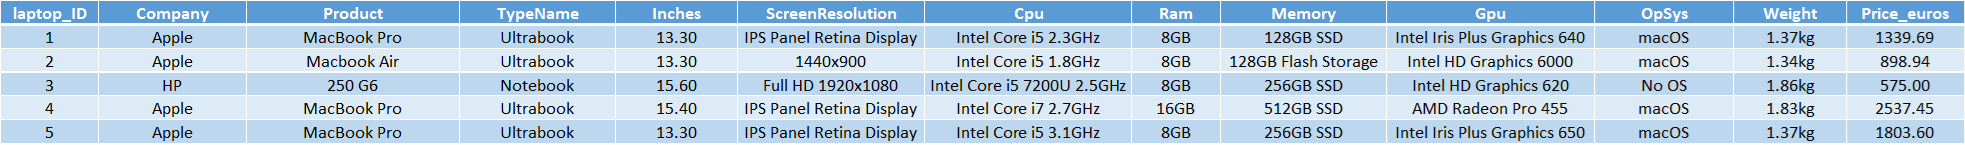
\includegraphics[scale = 0.4]{GambaR Tbale.png}
    \caption{5 Baris Pertama dari Data}
    \label{First}
\end{figure}  
  
Sedangkan jika data di-\textit{filter} menjadi 6 perusahaan dengan pangsa pasar terbesar yakni : HP, Lenovo, Dell, Asus, Acer dan Apple, data hanya memiliki 1150 baris dan 12 kolom. Pada bagian-bagian berikutnya, hanya data yang telah di-\textit{filter} yang akan dibahas.
\subsubsection{Company}
Kolom ini berisi nama perusahaan dari laptop. Pada kolom ini terdapat 19 perusahaan yang dalam pengolahannya akan di-\textit{filter}. Berikut dilampirkan banyaknya laptop dari 6 perusahaan.
\begin{figure}[h!]
    \centering
    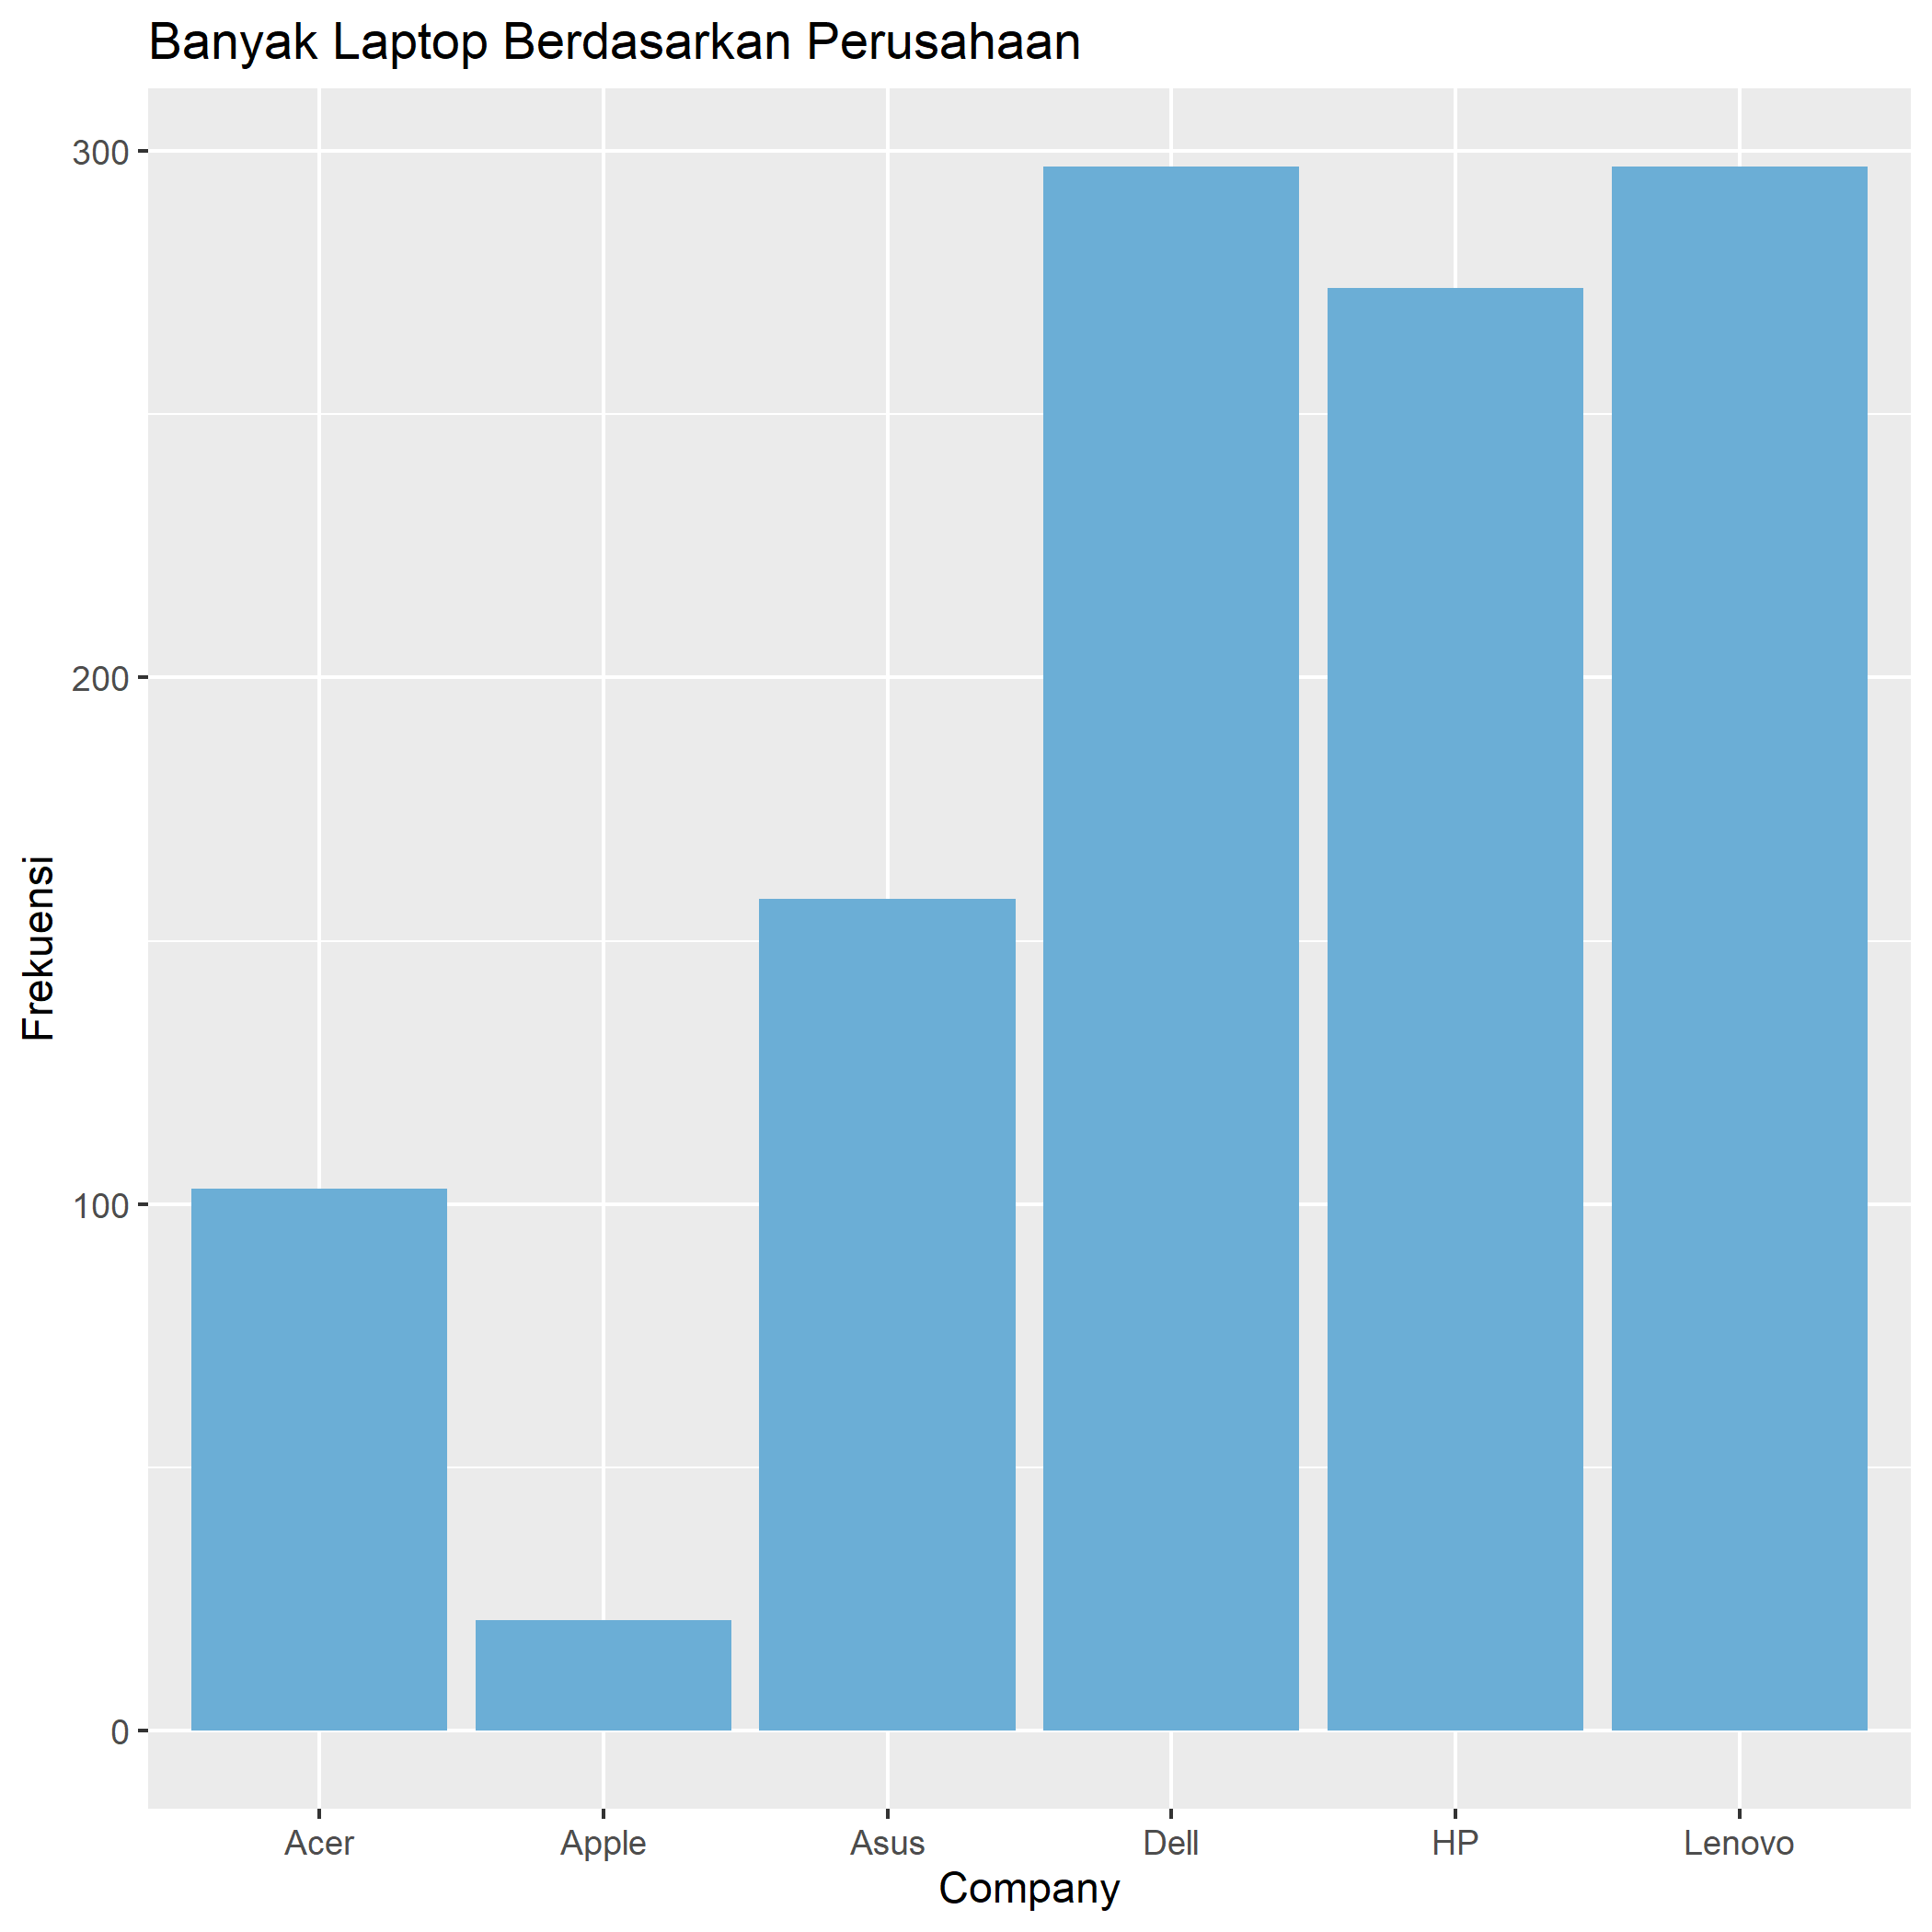
\includegraphics[scale = 0.4]{barplot0.png}
    \caption{Diagram Batang Laptop Berdasarkan Perusahaan}
    \label{ahay}
\end{figure}
\subsubsection{Product}
Kolom Product berisi nama produk atau seri dari laptop yang dijual. Terdapat 506 varian dari 6 perusahaan yang akan ditinjau. 
\subsubsection{TypeName}
Kolom TypeName berisi jenis laptop. Terdapat 6 jenis laptop yaitu Ultrabook, Notebook, Netbook, Gaming, 2 in 1 Convertible, dan Workstation. 
\begin{figure}[h!]
    \centering
    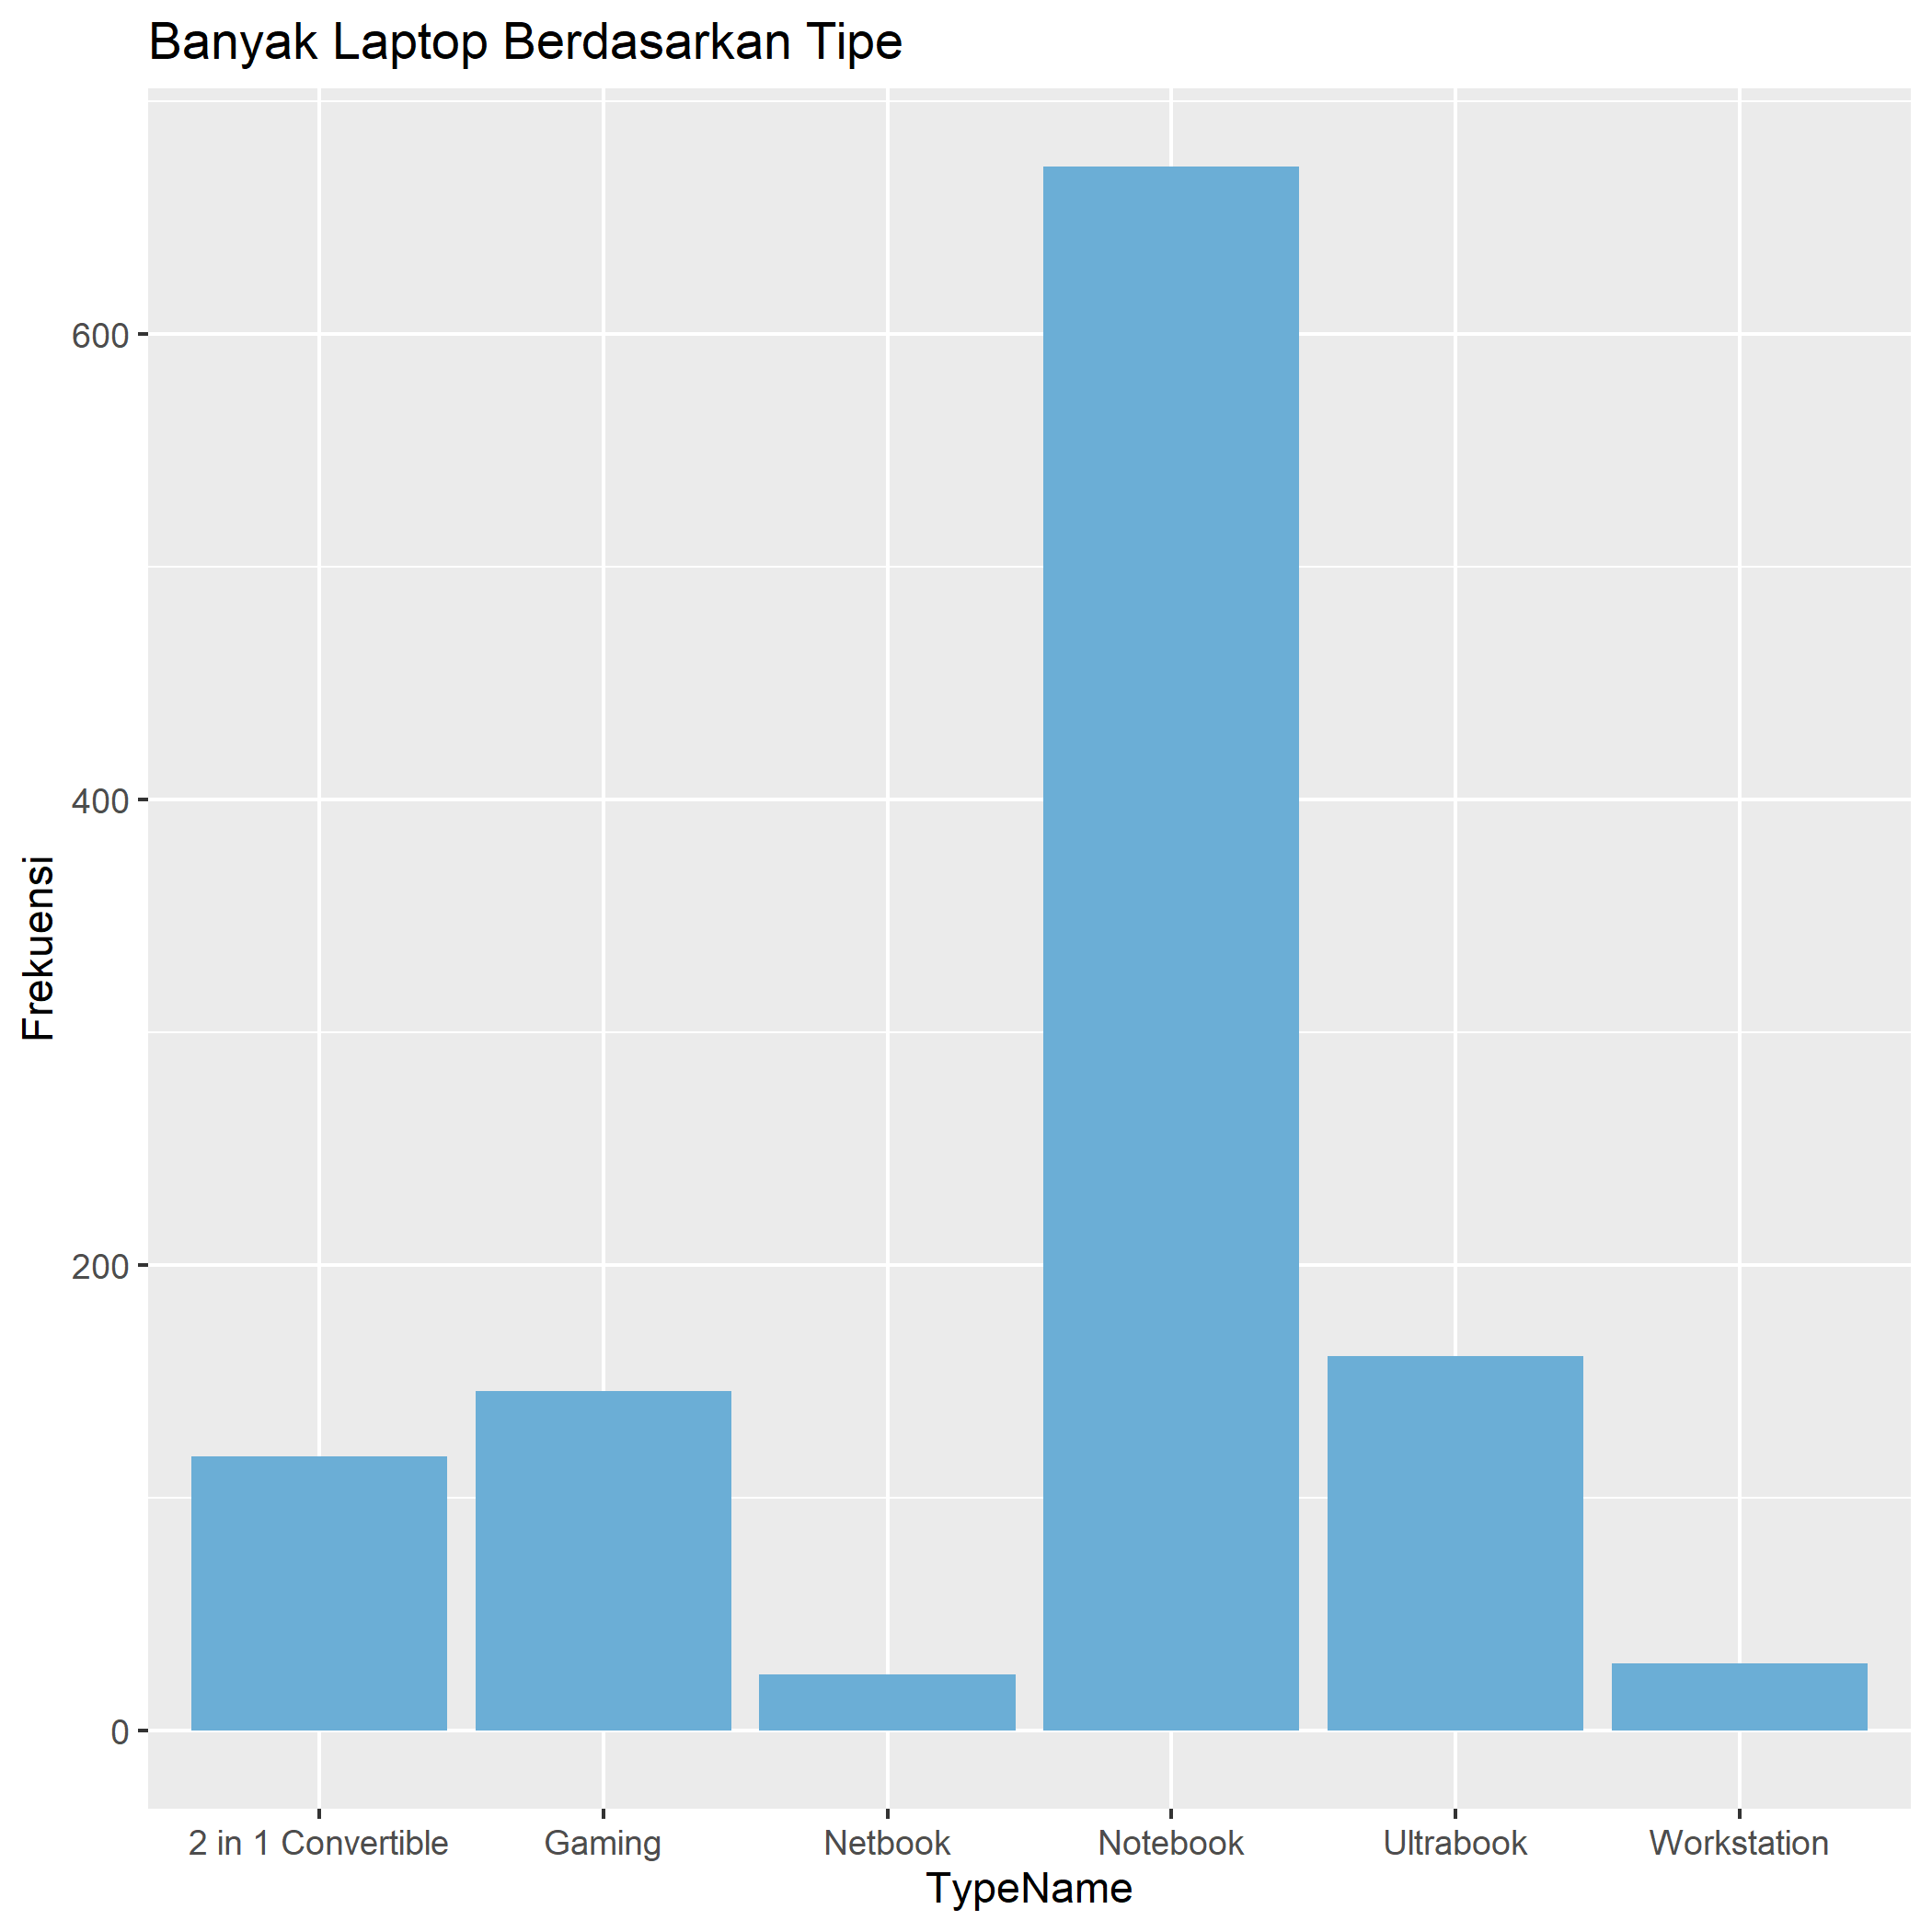
\includegraphics[scale = 0.4]{barplot1.png}
    \caption{Diagram Batang Laptop Berdasarkan Tipe}
    \label{ahay}
\end{figure}
\subsubsection{Inches}
Kolom Inches berisi ukuran laptop. Pada Gambar \ref{fig:ahayn}, hanya laptop dari perusahan ASUS yang tidak memiliki pencilan sedangkan pada perusahaan Lenovo memiliki pencilan paling banyak yaitu sebanyak 3. 
\begin{figure}[h!]
    \centering
    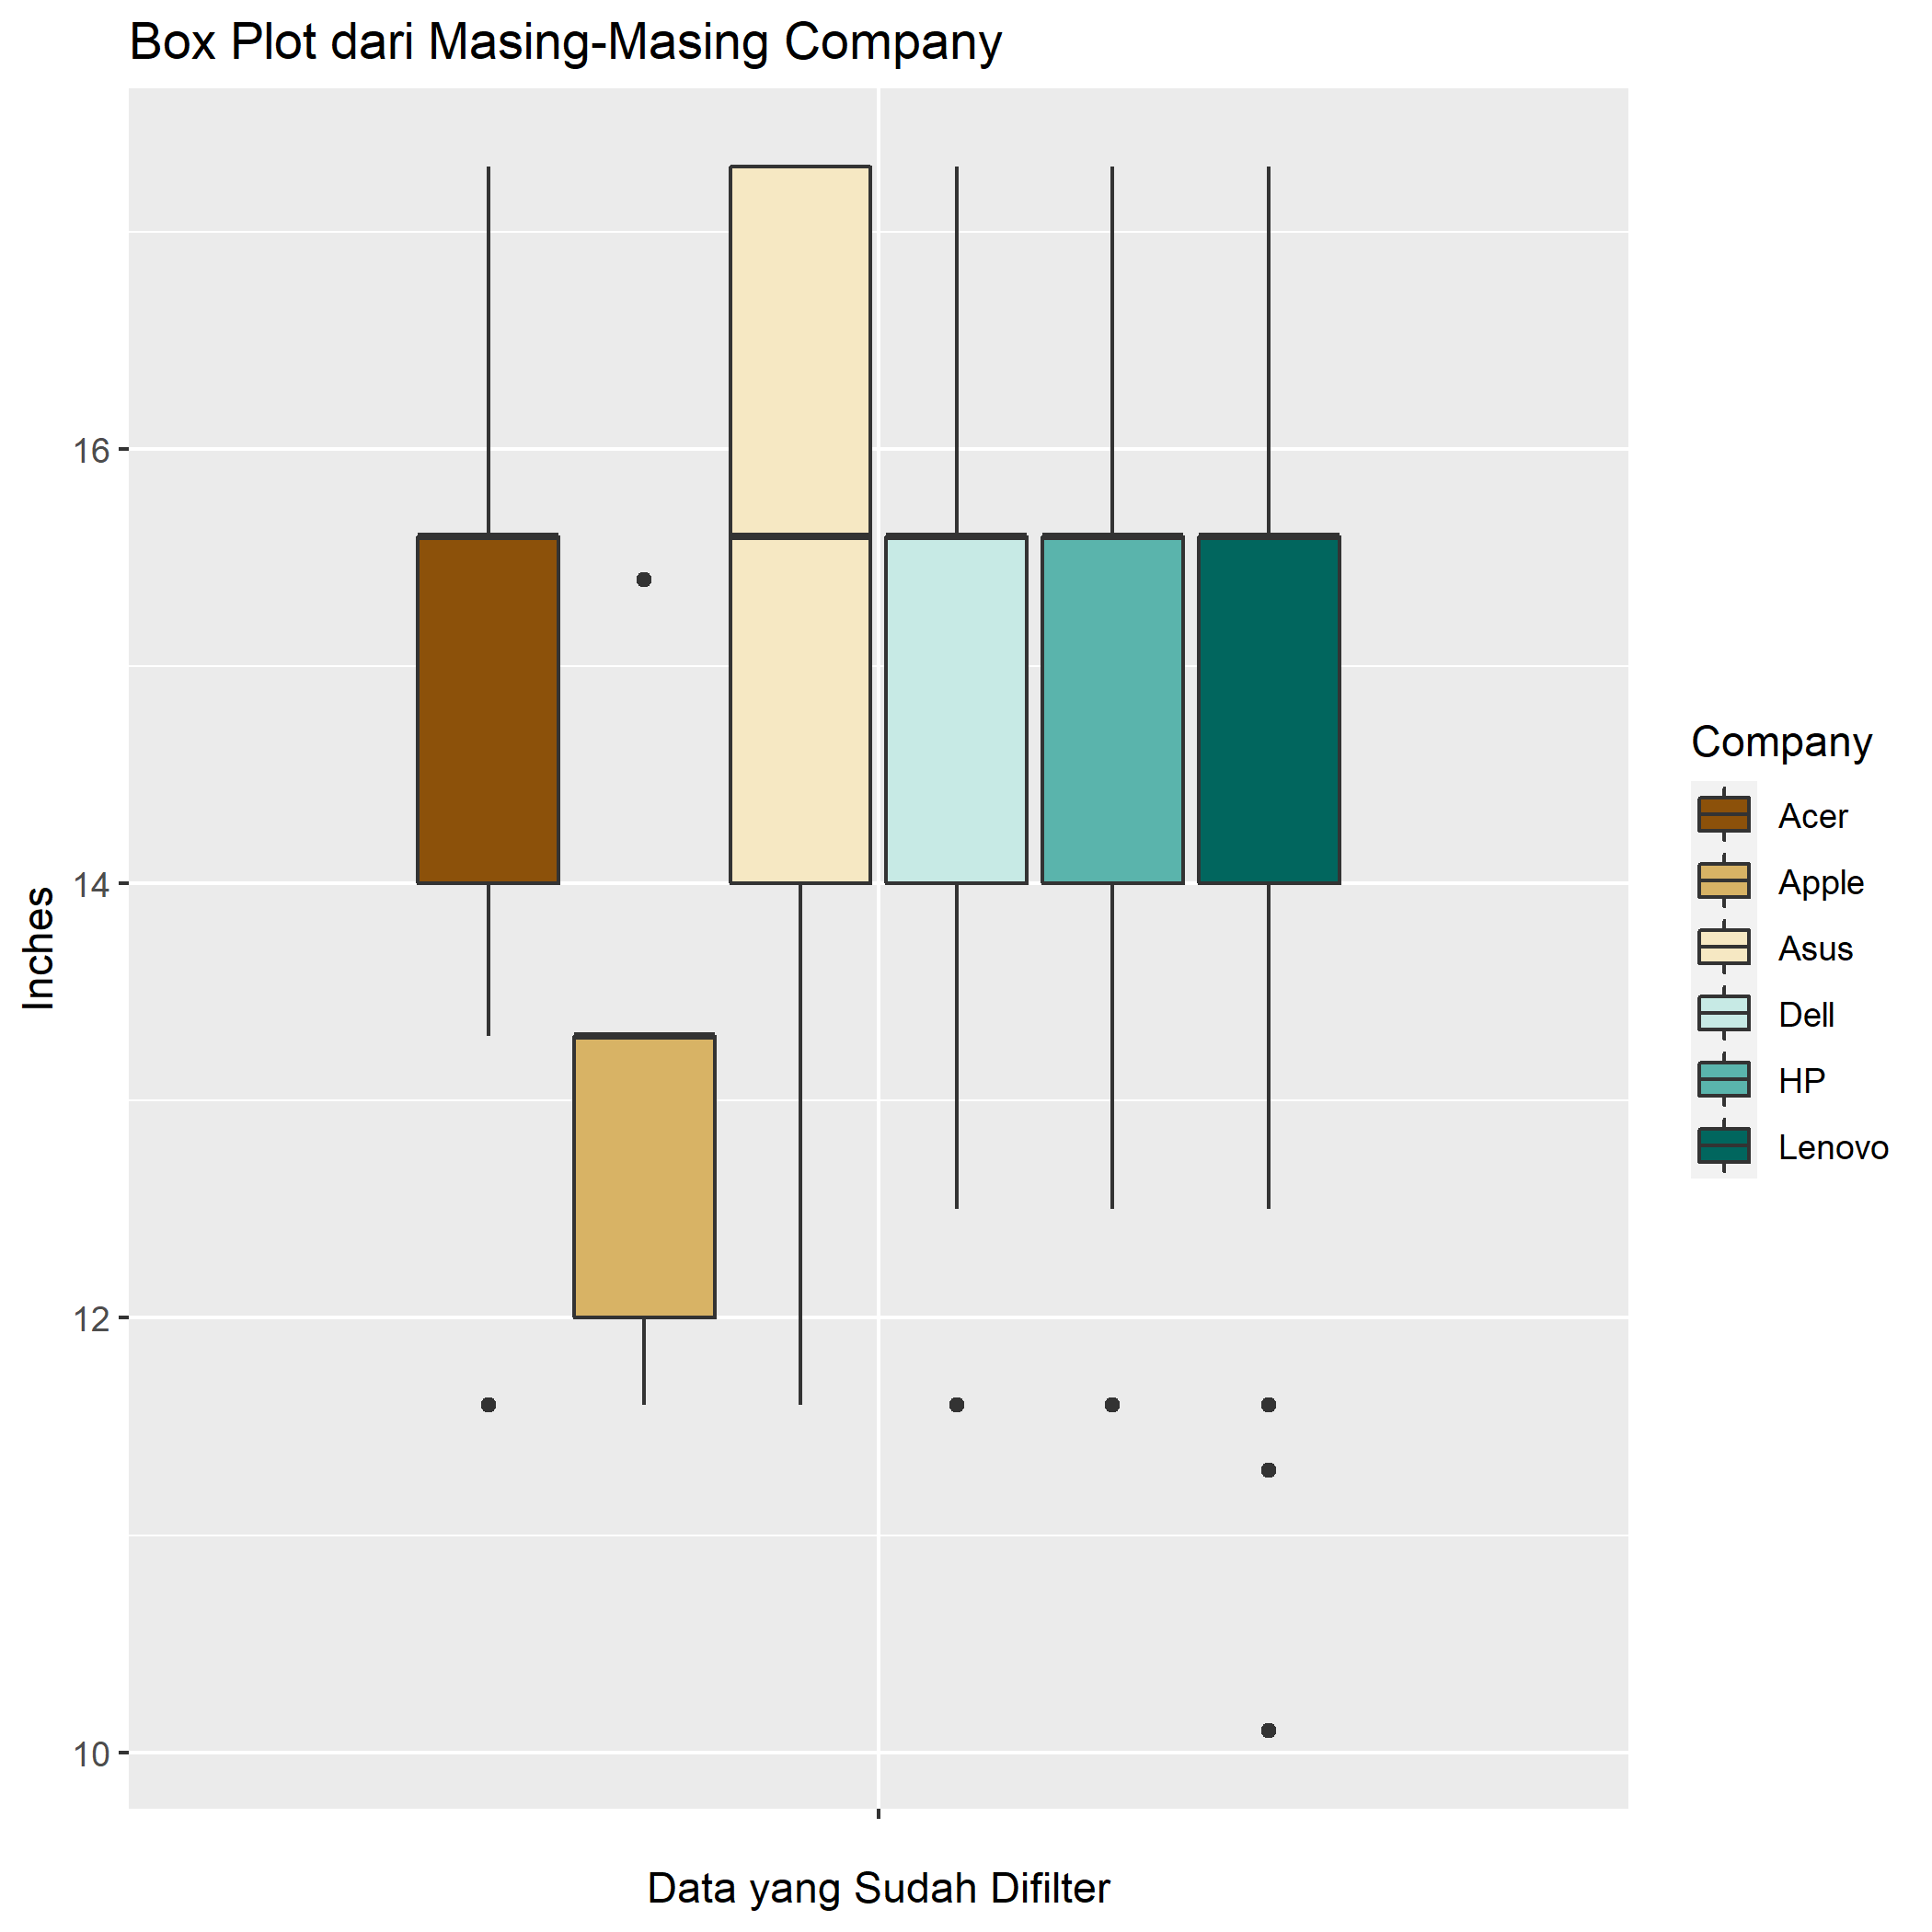
\includegraphics[scale = 0.4]{boxplot2.png}
    \caption{Diagram Kotak Garis Inches Laptop berdasarkan Perusahaan}
    \label{fig:ahayn}
\end{figure}
\subsubsection{Screen Resolution}
Kolom ini berisi jenis layar dan resolusi layar dari laptop. Pada data, terdapat 33 kombinasi dari jenis dan resolusi layar. Hanya saja ada entri data yang hanya memiliki resolusi layar saja dan ada juga entri data yang memiliki 2 jenis layar.
Sehingga akan dibersihkan lebih lanjut.
\subsubsection{Cpu}
Kolom Cpu berisi merk, seri dan kecepatan dari CPU laptop. Karena dalam 1 kolom berisi 3 buah informasi maka akan diolah lebih lanjut. 
\subsubsection{Ram}
Kolom Ram berisi ukuran RAM yang dimiliki oleh laptop. Pada kolom ini, entri dengan nilai minimum adalah 2GB dan nilai maksimum adalah 64GB. Perhatikan bahwa entri Ram memiliki karakteristik khusus yakni nilainya mengikut kombinasi $a2^n$ dengan $a\in \mathbb{N}$ dan $n \in \{0\} \cup \mathbb{N}$.
\subsubsection{Memory}
Kolom Memory berisi ukuran \textit{memory} atau \textit{storage} yang dimiliki oleh laptop. Pada kolom ini, terdapat 2 buah karakteristik yang cukup mencolok yaitu ada kolom yang berisi 2 buah memory dengan tipe dan ukuran yang berbeda sehingga perlu diolah lebih lanjut. 
\subsubsection{Gpu}
Kolom Gpu berisi merk, dan seri GPU laptop. Karena dalam 1 kolom berisi 2 buah informasi maka akan diolah lebih lanjut. 
\subsubsection{OpSys}
Kolom OpSys berisi \textit{Operating System} laptop. Terdapat 9 jenis \textit{Operating System} yang dimiliki oleh laptop dengan pesebarannya seperti berikut 
\begin{figure}[h!]
    \centering
    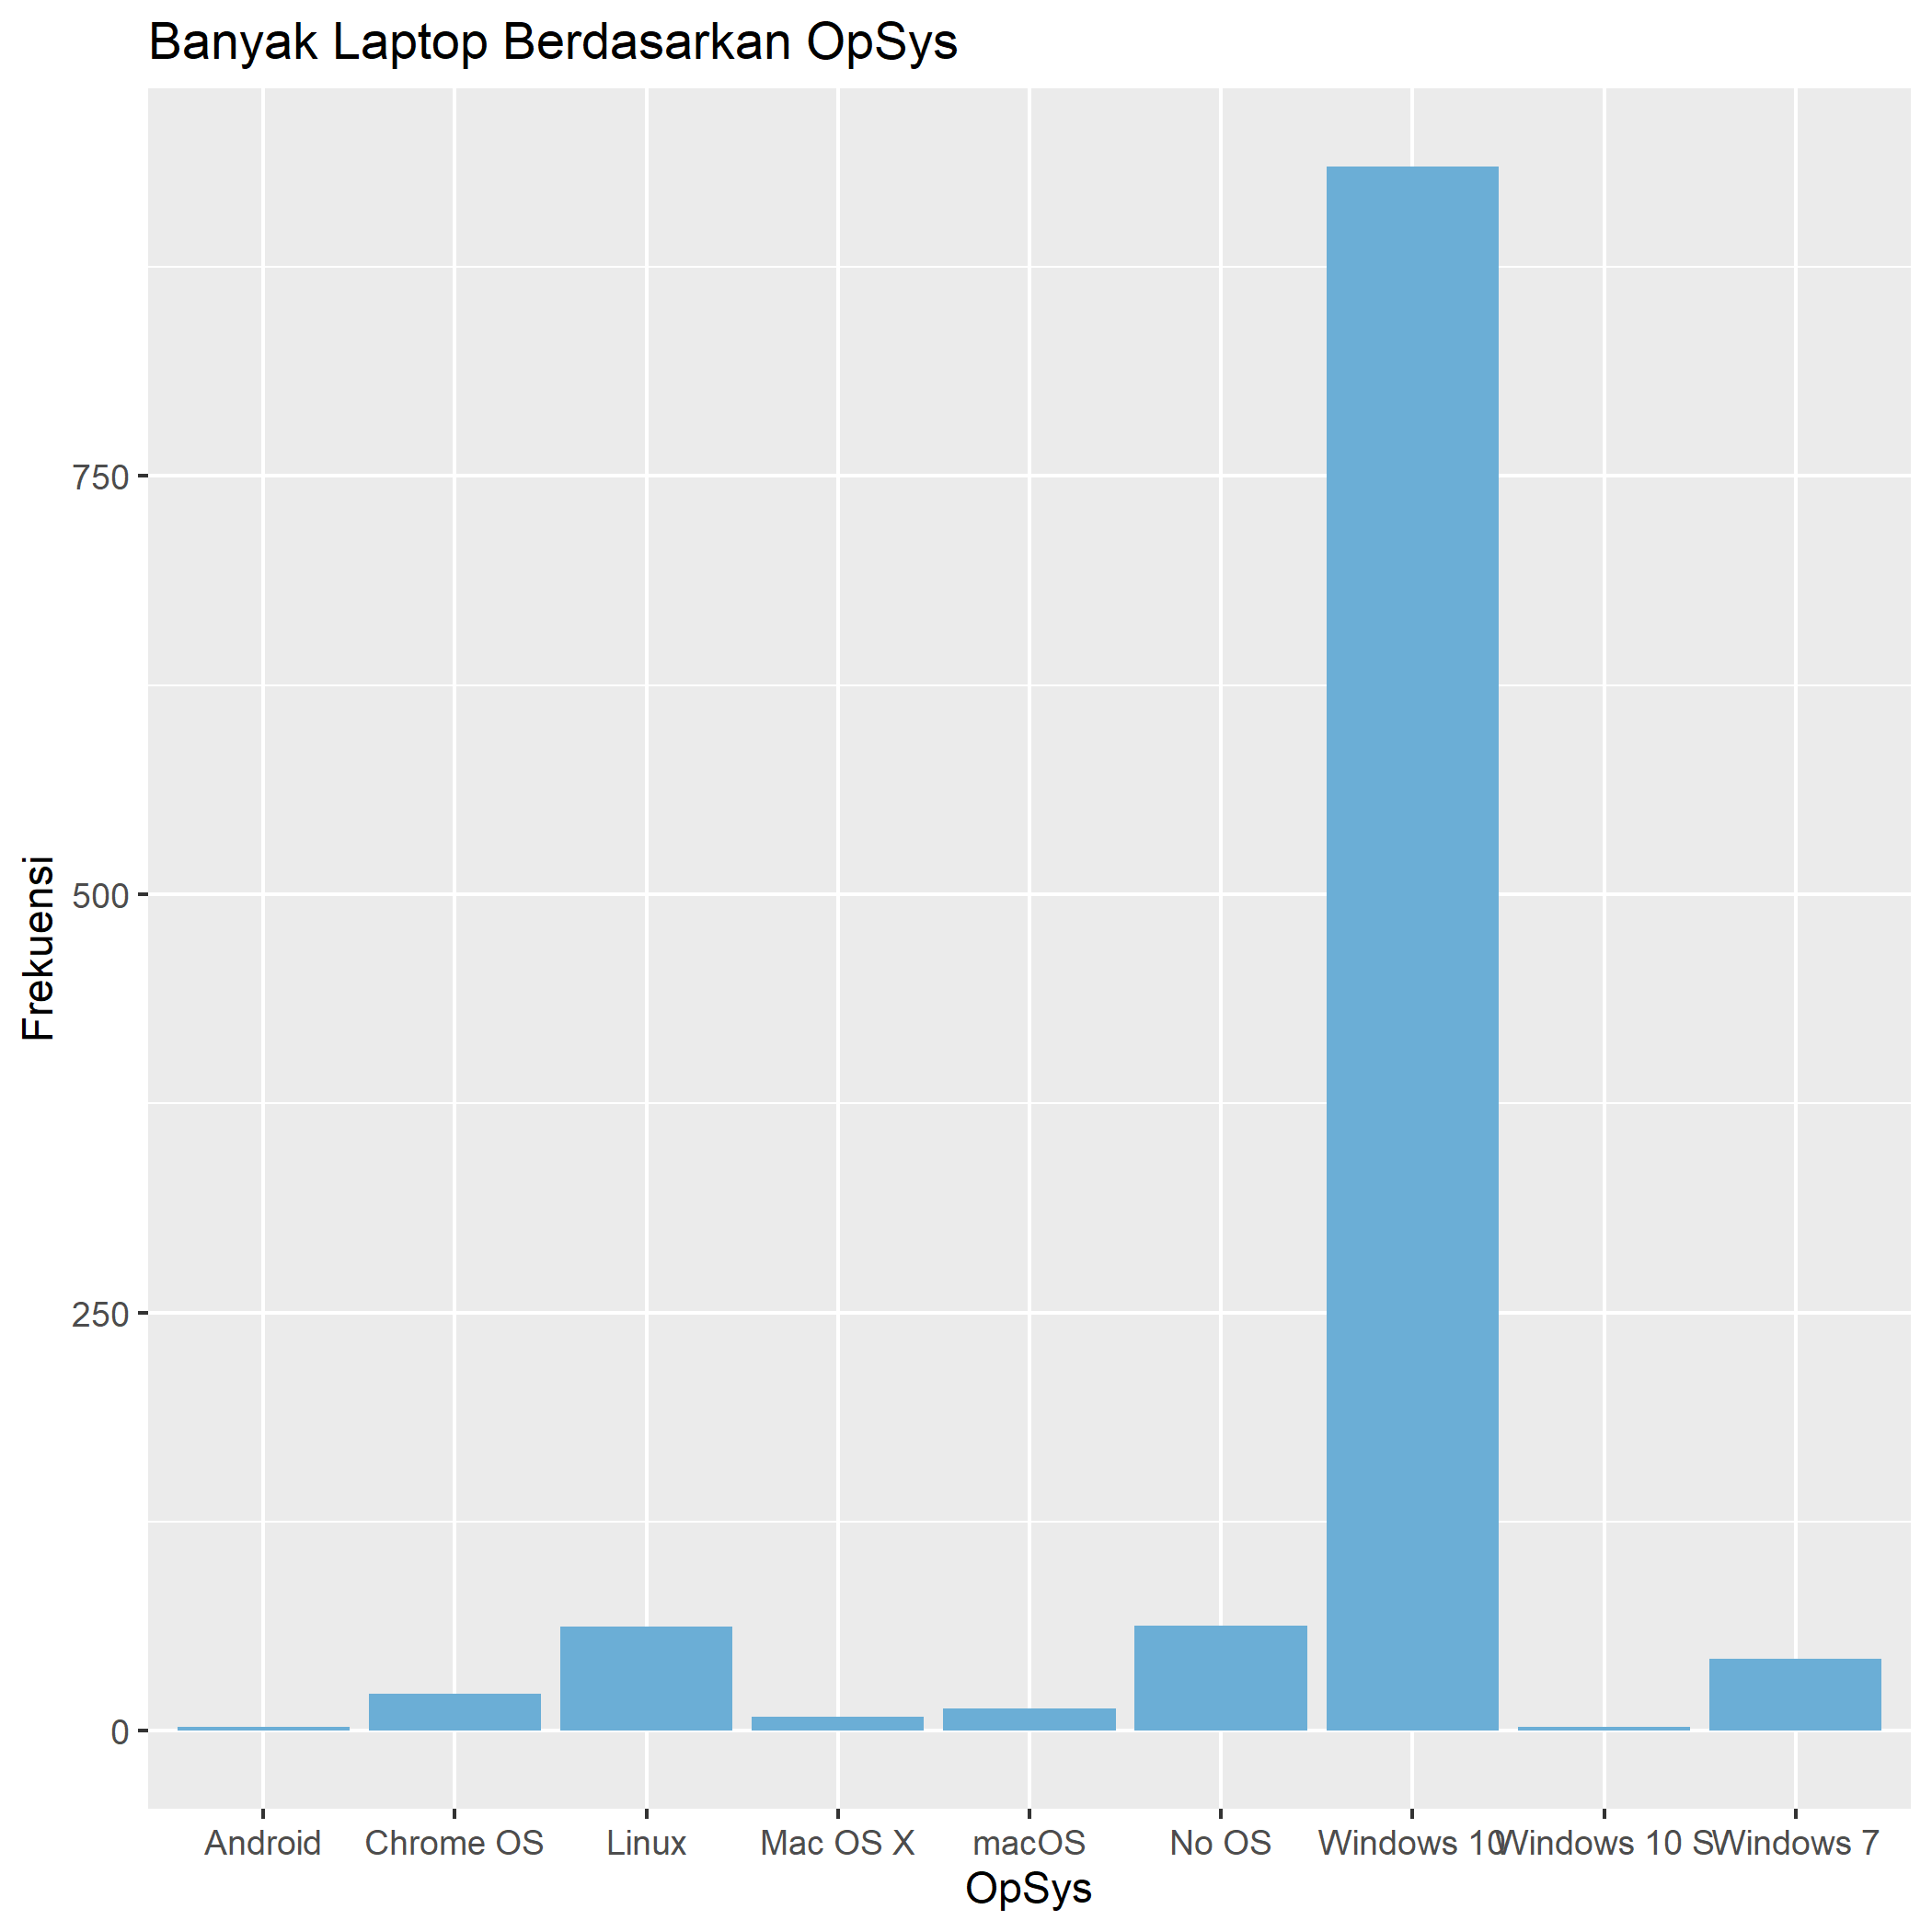
\includegraphics[scale = 0.4]{barplot2.png}
    \caption{Diagram Batang Laptop berdasarkan \textit{Operating System}}
    \label{ahay}
\end{figure}
\subsubsection{Weight}
Kolom Weight berisi bobot atau berat laptop. Pada data dapat dilihat bahwa data berupa \textit{string} sehingga perlu dibersihkan terlebih dahulu.
\subsubsection{Price\_euros}
Kolom Price\_euros berisi harga laptop dengan mata uang Euro. Perhatikan bahwa distribusi dari data \textit{skewed to the right}. 
\begin{figure}[h!]
    \centering
    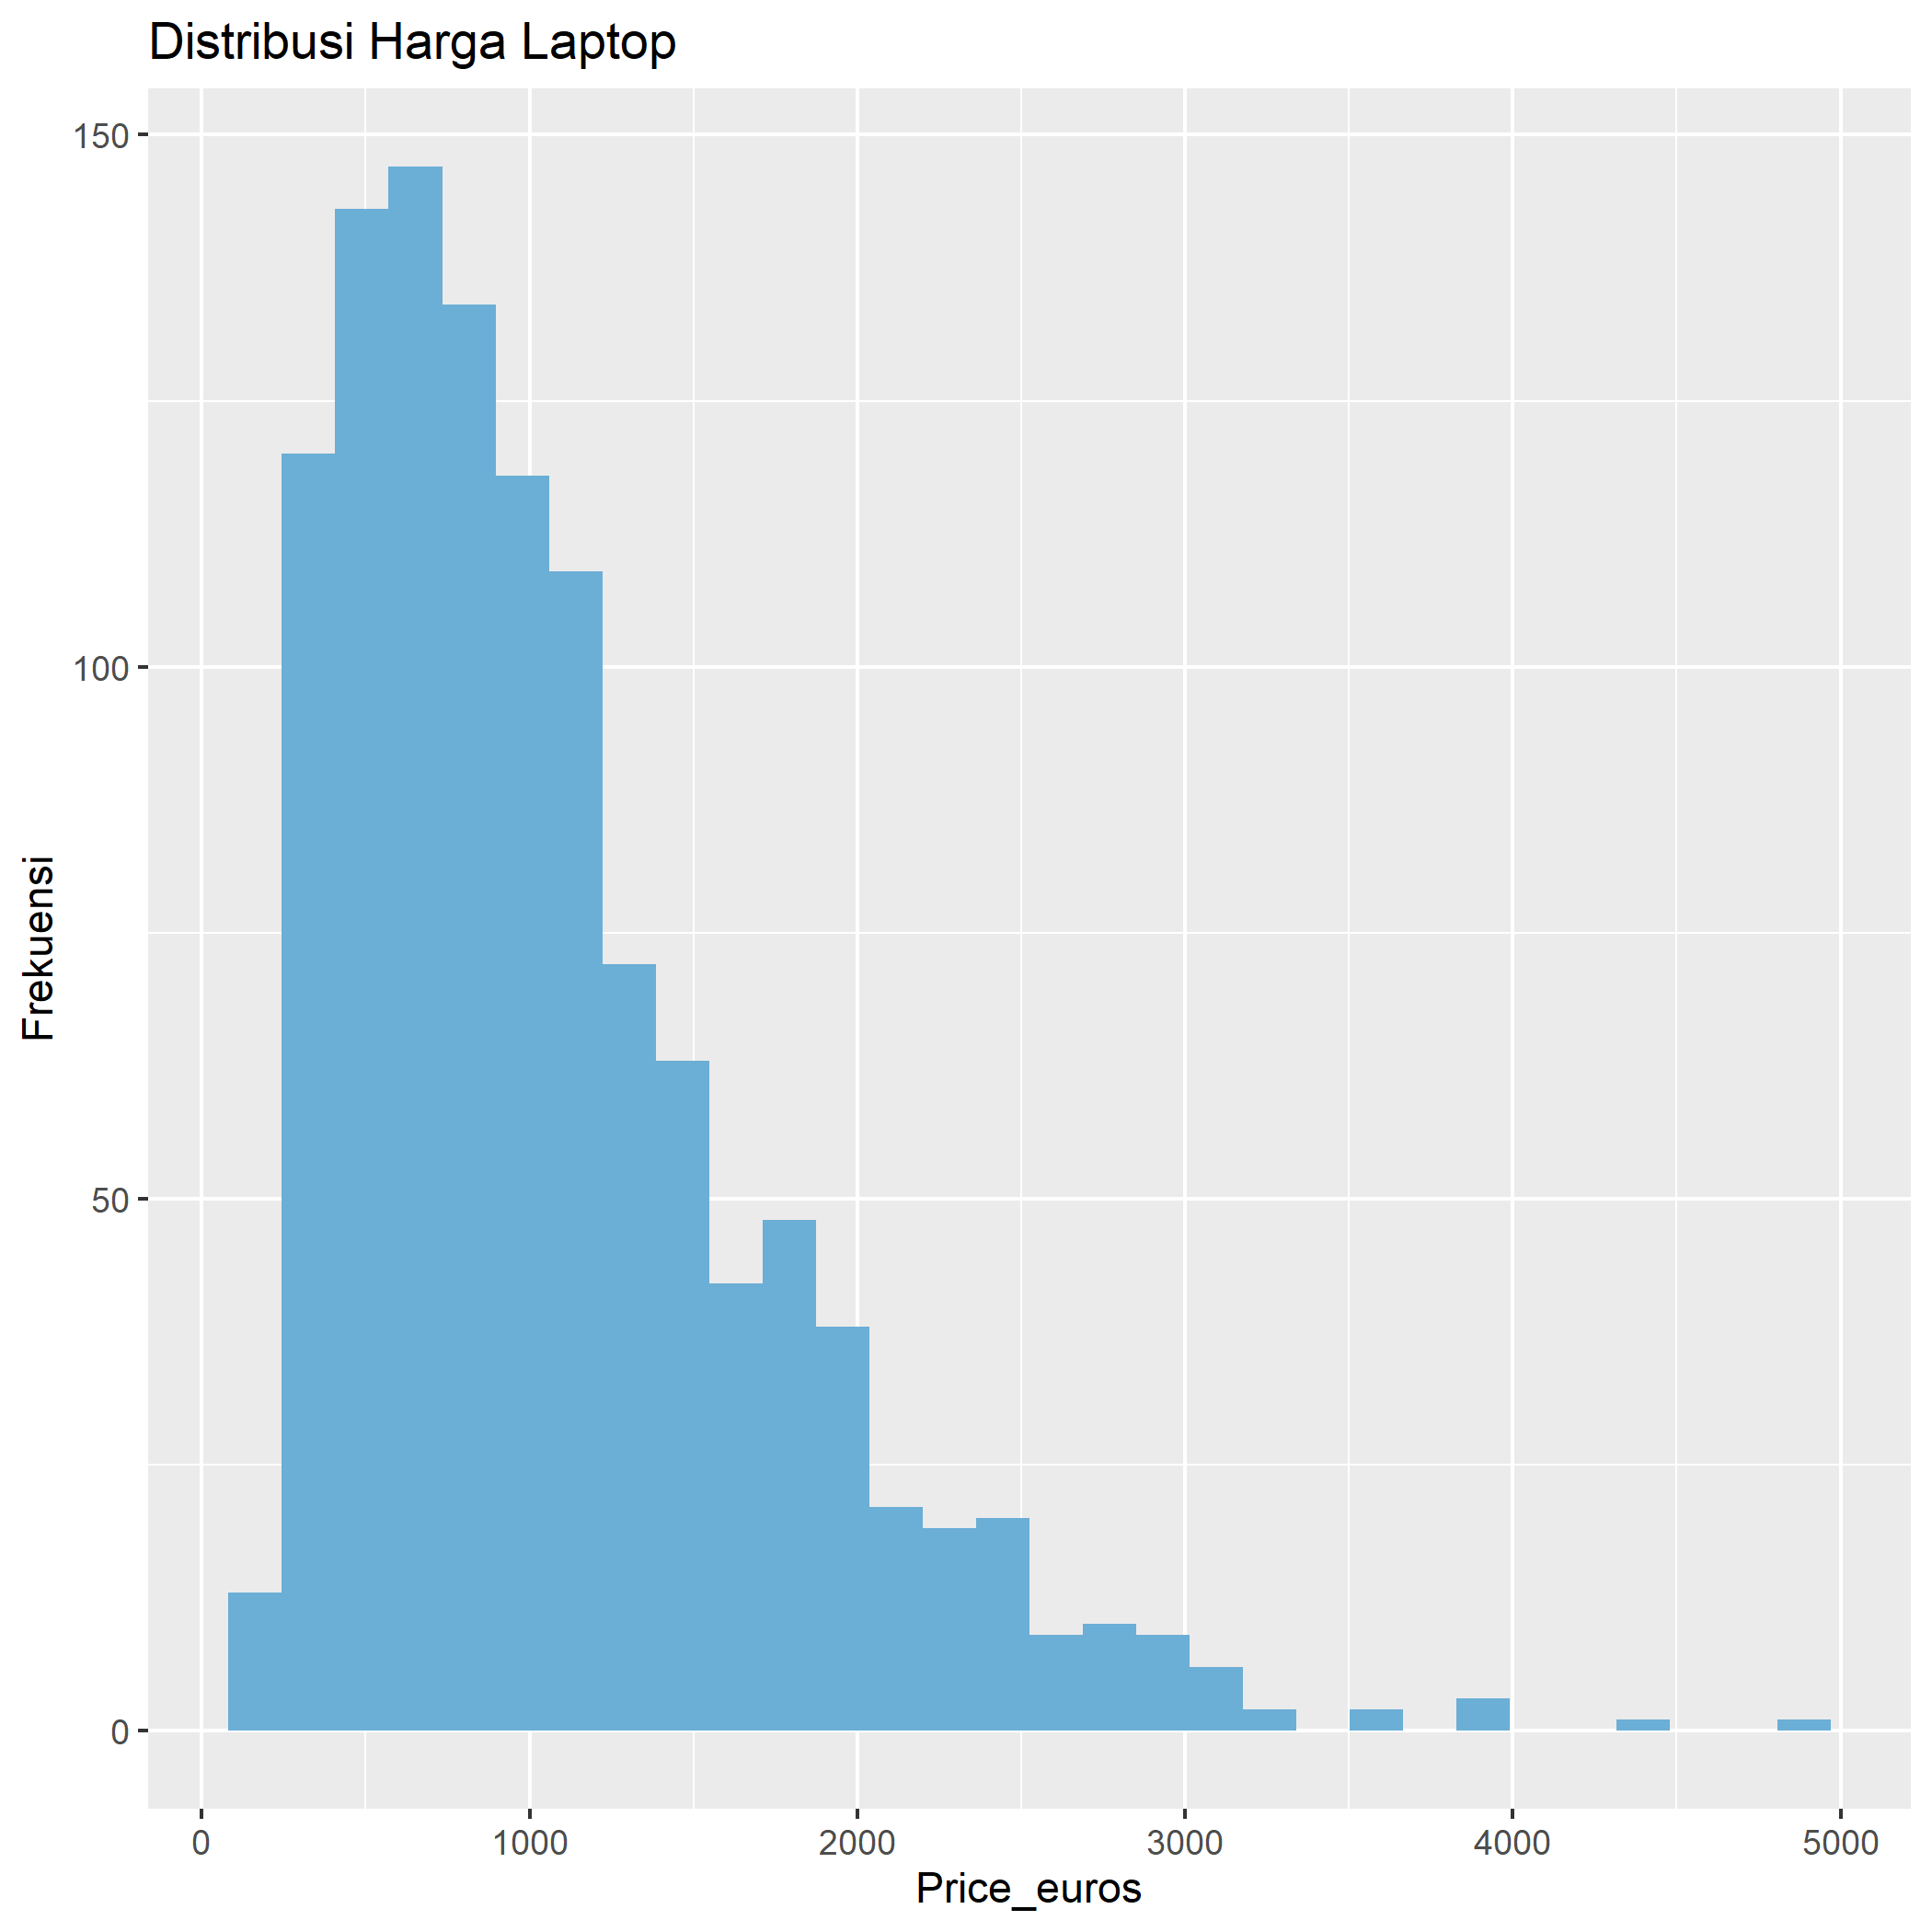
\includegraphics[scale = 0.4]{distplot.png}
    \caption{Histogram Harga Laptop }
    \label{ahay}
\end{figure}
\newpage
\subsection{Pembersihan Data / \textit{Data Cleaning}}
Seperti yang telah dijelaskan sebelumnya, pada bagian ini akan dijelaskan bagaimana cara data pada kolom tersebut 'dibersihkan'.
\subsubsection{Screen Resolution}
Pada kolom ini akan dibuat kolom baru dengan nama ScreenType. Jika pada kolom hanya terdapat 1 kata saja (contohnya seperti 1920x1200) maka ScreenType akan diisi dengan ' ' pada kolom ScreenResolution dan ScreenType akan dibuat menjadi tipe \textit{factor}. Alasannya karena ukuran resolusi tidak bisa diubah-ubah sesuai keiinginan dan juga pada kolom ScreenResolution akan dipilih 1920x1080 sebagai \textit{base level} dan pada ScreenType akan dipilih Full HD sebagai \textit{base level}.
\subsubsection{Cpu}
Pada kolom ini akan dibuat 3 buah kolom baru dengan nama Cpu\_Type, Cpu\_Series dan Cpu\_Speed. Pada kolom Cpu terdapat suatu pola yang memudahkan untuk mengelompokkan masing-masing entri. Kata pertama adalah tipe dari CPUnya dan kata terakhir adalah kecepatan dari CPUnya. Sedangkan kata yang berada diantaranya adalah Seri dari CPUnya. Contohnya dapat dilihat pada grafik dibawah ini   
  
\begin{figure}[h!]
    \centering
    \begin{tikzpicture}[node distance=2cm]
    \node (Cpu) [startstop] {Intel Core i5 7200U 2.5GHz};
    \node (CpuType) [startstop, below of = Cpu, xshift = -5cm] {Intel};
    \node (CpuSeries) [startstop, below of = Cpu] {Core i5 7200U};
    \node (CpuSpeed) [startstop, below of = Cpu,xshift = 5cm] {2.5GHz};
    \draw [arrow] (Cpu) -- (CpuType);
    \draw [arrow] (Cpu) -- (CpuSeries);
    \draw [arrow] (Cpu) -- (CpuSpeed);
    \end{tikzpicture}
    \caption{Contoh Membersihkan Kolom Cpu}
    \label{clean_cpu}
\end{figure}
  
\newpage
3 buah kolom baru ini akan diubah ke \textit{format} \textit{factor} dan \textit{numeric}. Akan dipilih Intel sebagai \textit{base level} dari Cpu\_Type, Core i5 7200U sebagai \textit{base level} dari Cpu\_Series dan Cpu\_Speed akan diubah ke format \textit{numeric} setelah kata 'GHz' dihilangkan.   
\subsubsection{Ram}
Pada kolom Ram cukup menghilangkan kata 'GB' dari kolom dan juga mengubahnya ke dalam bentuk \textit{numeric}. 
\subsubsection{Memory}
Pada kolom ini akan dibagi terlebih dahulu menjadi 2 bagian dan kemudian akan dipisahkan kembali berdasarkan ukuran dan tipenya. Contohnya dapat dilihat pada grafik dibawah ini

\begin{figure}[h!]
    \centering
    \begin{tikzpicture}[node distance=2cm]
    \node (Memory) [startstop] {128GB SSD +  1TB HDD};
    \node (Memory1) [startstop, below of = Memory, xshift = -4.5cm] {128GB SSD};
    \node (Memory2) [startstop, below of = Memory,xshift = 4.5cm] {1 TB HDD};
    \node (Memory1Size) [startstop, below of = Memory1, xshift = -2.5cm] {128GB};
    \node (Memory1Type) [startstop, below of = Memory1, xshift = 2.5cm] {SSD};
    \node (Memory2Size) [startstop, below of = Memory2,xshift = -2.5cm] {1 TB};
    \node (Memory2Type) [startstop, below of = Memory2,xshift = 2.5cm] {HDD};
    \draw [arrow] (Memory) -- (Memory1);
    \draw [arrow] (Memory) -- (Memory2);
    \draw [arrow] (Memory1) -- (Memory1Size);
    \draw [arrow] (Memory1) -- (Memory1Type);
    \draw [arrow] (Memory2) -- (Memory2Size);
    \draw [arrow] (Memory2) -- (Memory2Type);
    \end{tikzpicture}
    \caption{Contoh Membersihkan Kolom Memory}
    \label{clean_memory}
\end{figure}
Perhatikan bahwa tidak semua laptop memiliki 2 memori sehingga untuk tiap komputer yang tidak memiliki memori kedua akan diberi label ' '. Pada kolom Memory\_1\_Size dan Memory\_2\_Size ditemukan juga bentuk 1.0 TB dan 1TB sehingga perlu disamakan terlebih dahulu. Berikutnya akan dikonversi semua ukuran TB menjadi GB (1TB = 1024 GB) kemudian akan dihilangkan kata GB pada tiap kolom Size dan akan diubah ke format \textit{numeric}.  Perhatikan juga pada umumnya ukuran dari \textit{memory} mengikuti bentuk $2^n$ hanya saja dewasa ini, ukurannya sudah mulai bervariasi jadi tidak menjadi suatu masalah untuk mengubahnya ke format \textit{numeric}. Sedangkan untuk  Memory\_1\_Type dan Memory\_2\_Type akan diubah ke format \textit{factor} dengan SSD sebagai \textit{base level} untuk kolom Memory\_1\_Type dan ' ' sebagai \textit{base level} Memory\_2\_Type.
\subsubsection{Gpu}
Sama halnya dengan kolom Cpu, pada kolom ini akan dibuat 2 buah kolom baru dengan nama Gpu\_Type dan Gpu\_Series. Pada kolom Gpu cukup dipisahkan kata pertama dari sisa kata yang lain. Karena kata pertama adalah tipe GPUnya sedangkan yang lain adalah seri dari GPUnya. Contohnya dapat dilihat pada grafik dibawah ini :  
  
\begin{figure}[h!]
    \centering
    \begin{tikzpicture}[node distance=2cm]
    \node (Gpu) [startstop] {Nvidia GeForce MX150};
    \node (GpuType) [startstop, below of = Gpu, xshift = -2.5cm] {Nvidia};
    \node (GpuSeries) [startstop, below of = Gpu,xshift = 2.5cm] {GeForce MX150};
    \draw [arrow] (Gpu) -- (GpuType);
    \draw [arrow] (Gpu) -- (GpuSeries);
    \end{tikzpicture}
    \caption{Contoh Membersihkan Kolom Gpu}
    \label{clean_cpu}
\end{figure}  
  
2 kolom yang baru dibuat ini nantinya akan dibuat menjadi bentuk \textit{factor} dengan Intel sebagai \textit{base level} pada kolom Gpu\_Type dan HD Graphics 620 sebagai \textit{base level} dari kolom Gpu\_Series.
\subsubsection{Weight}
Pada kolom Weight cukup menghilangkan kata 'kg' dari kolom dan juga mengubahnya ke dalam bentuk \textit{numeric}. 
\subsection{\textit{Exploratory Data Analysis} (EDA)}
\subsubsection{Hubungan antara Harga Laptop dengan ScreenResolution dan ScreenType }
Pada Diagram Kotak Garis dibawah ini dapat dilihat bahwa secara umum semakin besar resolusi laptop maka semakin besar pula range harganya. Hanya saja pada resolusi 1920x1080 terdapat banyak sekali pencilan atasnya. Hal ini wajar karena bisa saja laptop tersebut menawarkan piranti keras lain yang berbeda dari laptop dengan ScreenResolution yang sama.   
  
\begin{figure}[h!]
    \centering
    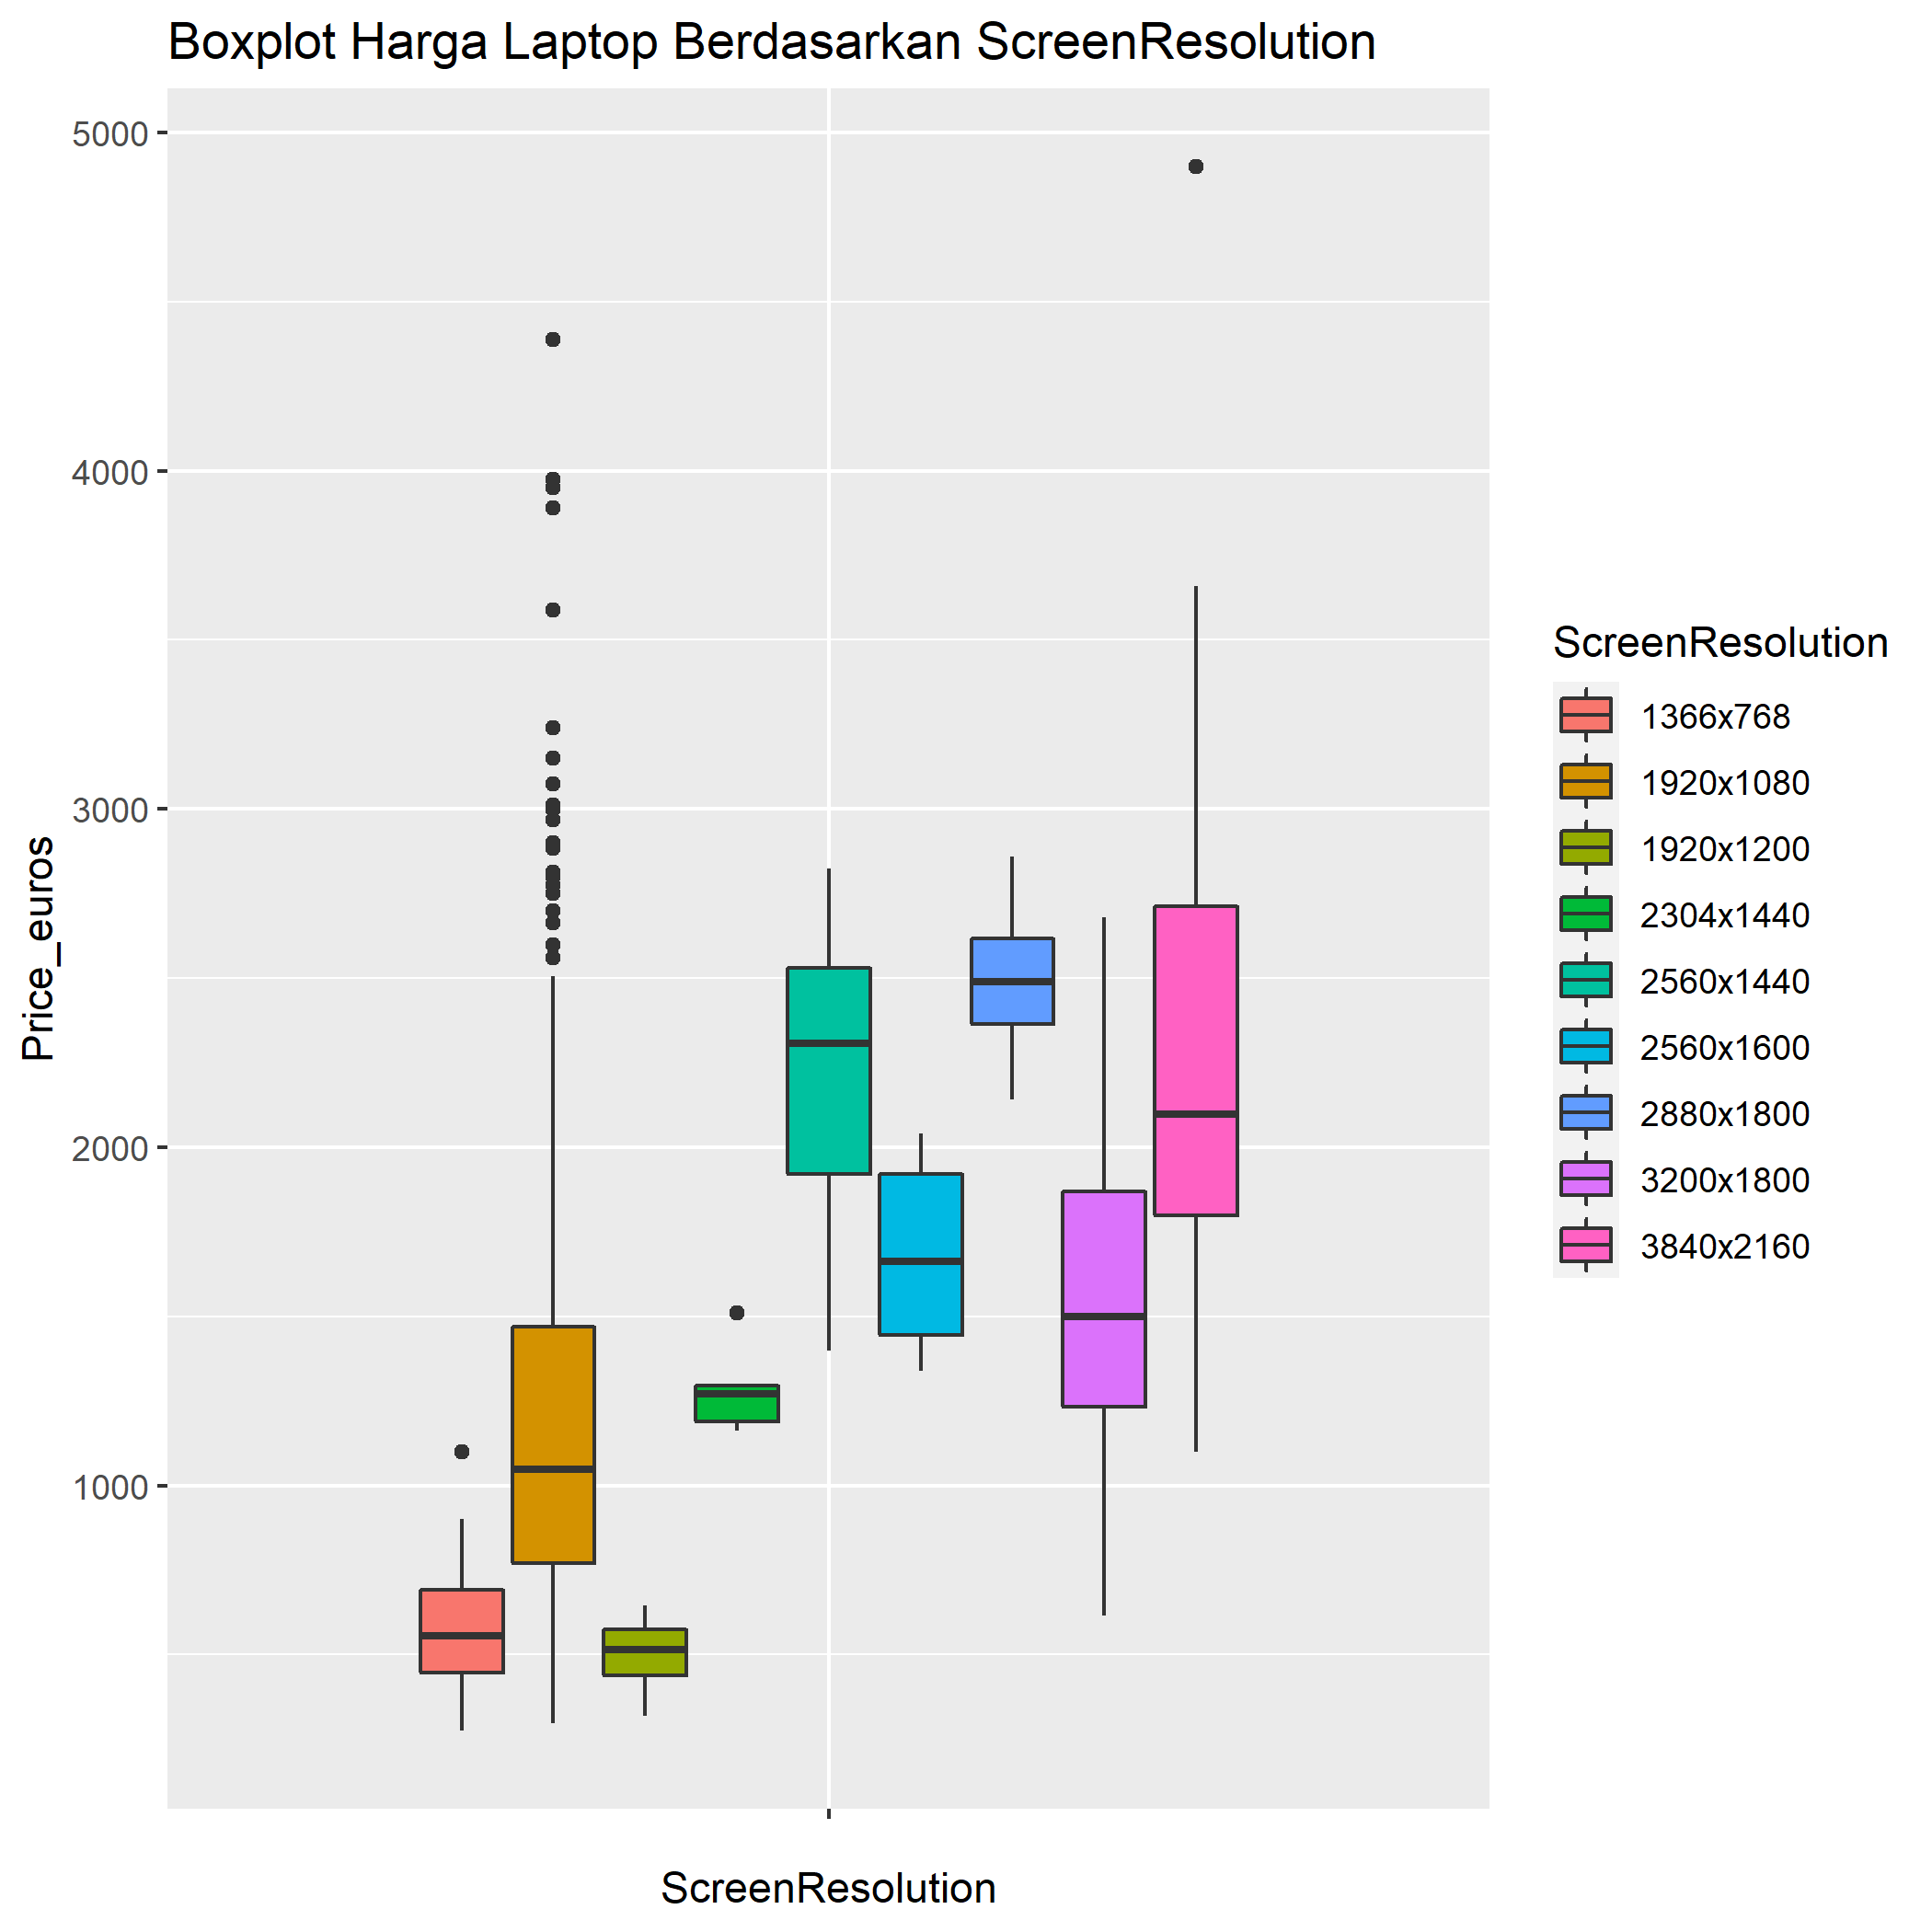
\includegraphics[scale = 0.4]{boxplot_price1.png}
    \caption{Diagram Kotak Garis Harga Berdasarkan ScreenResolution}
    \label{Resol}
\end{figure}  
  
Sedangkan jika dilihat Diagram Kotak Garis Harga Laptop Berdasarkan ScreenType dapat dilihat bahwa ScreenType dengan range yang paling tinggi adalah IPS Panel dan ScreenType yang memiliki Harga paling mahal adalah ScreenType IPS Panel 4K Ultra HD.  
  
\begin{figure}[h!]
    \centering
    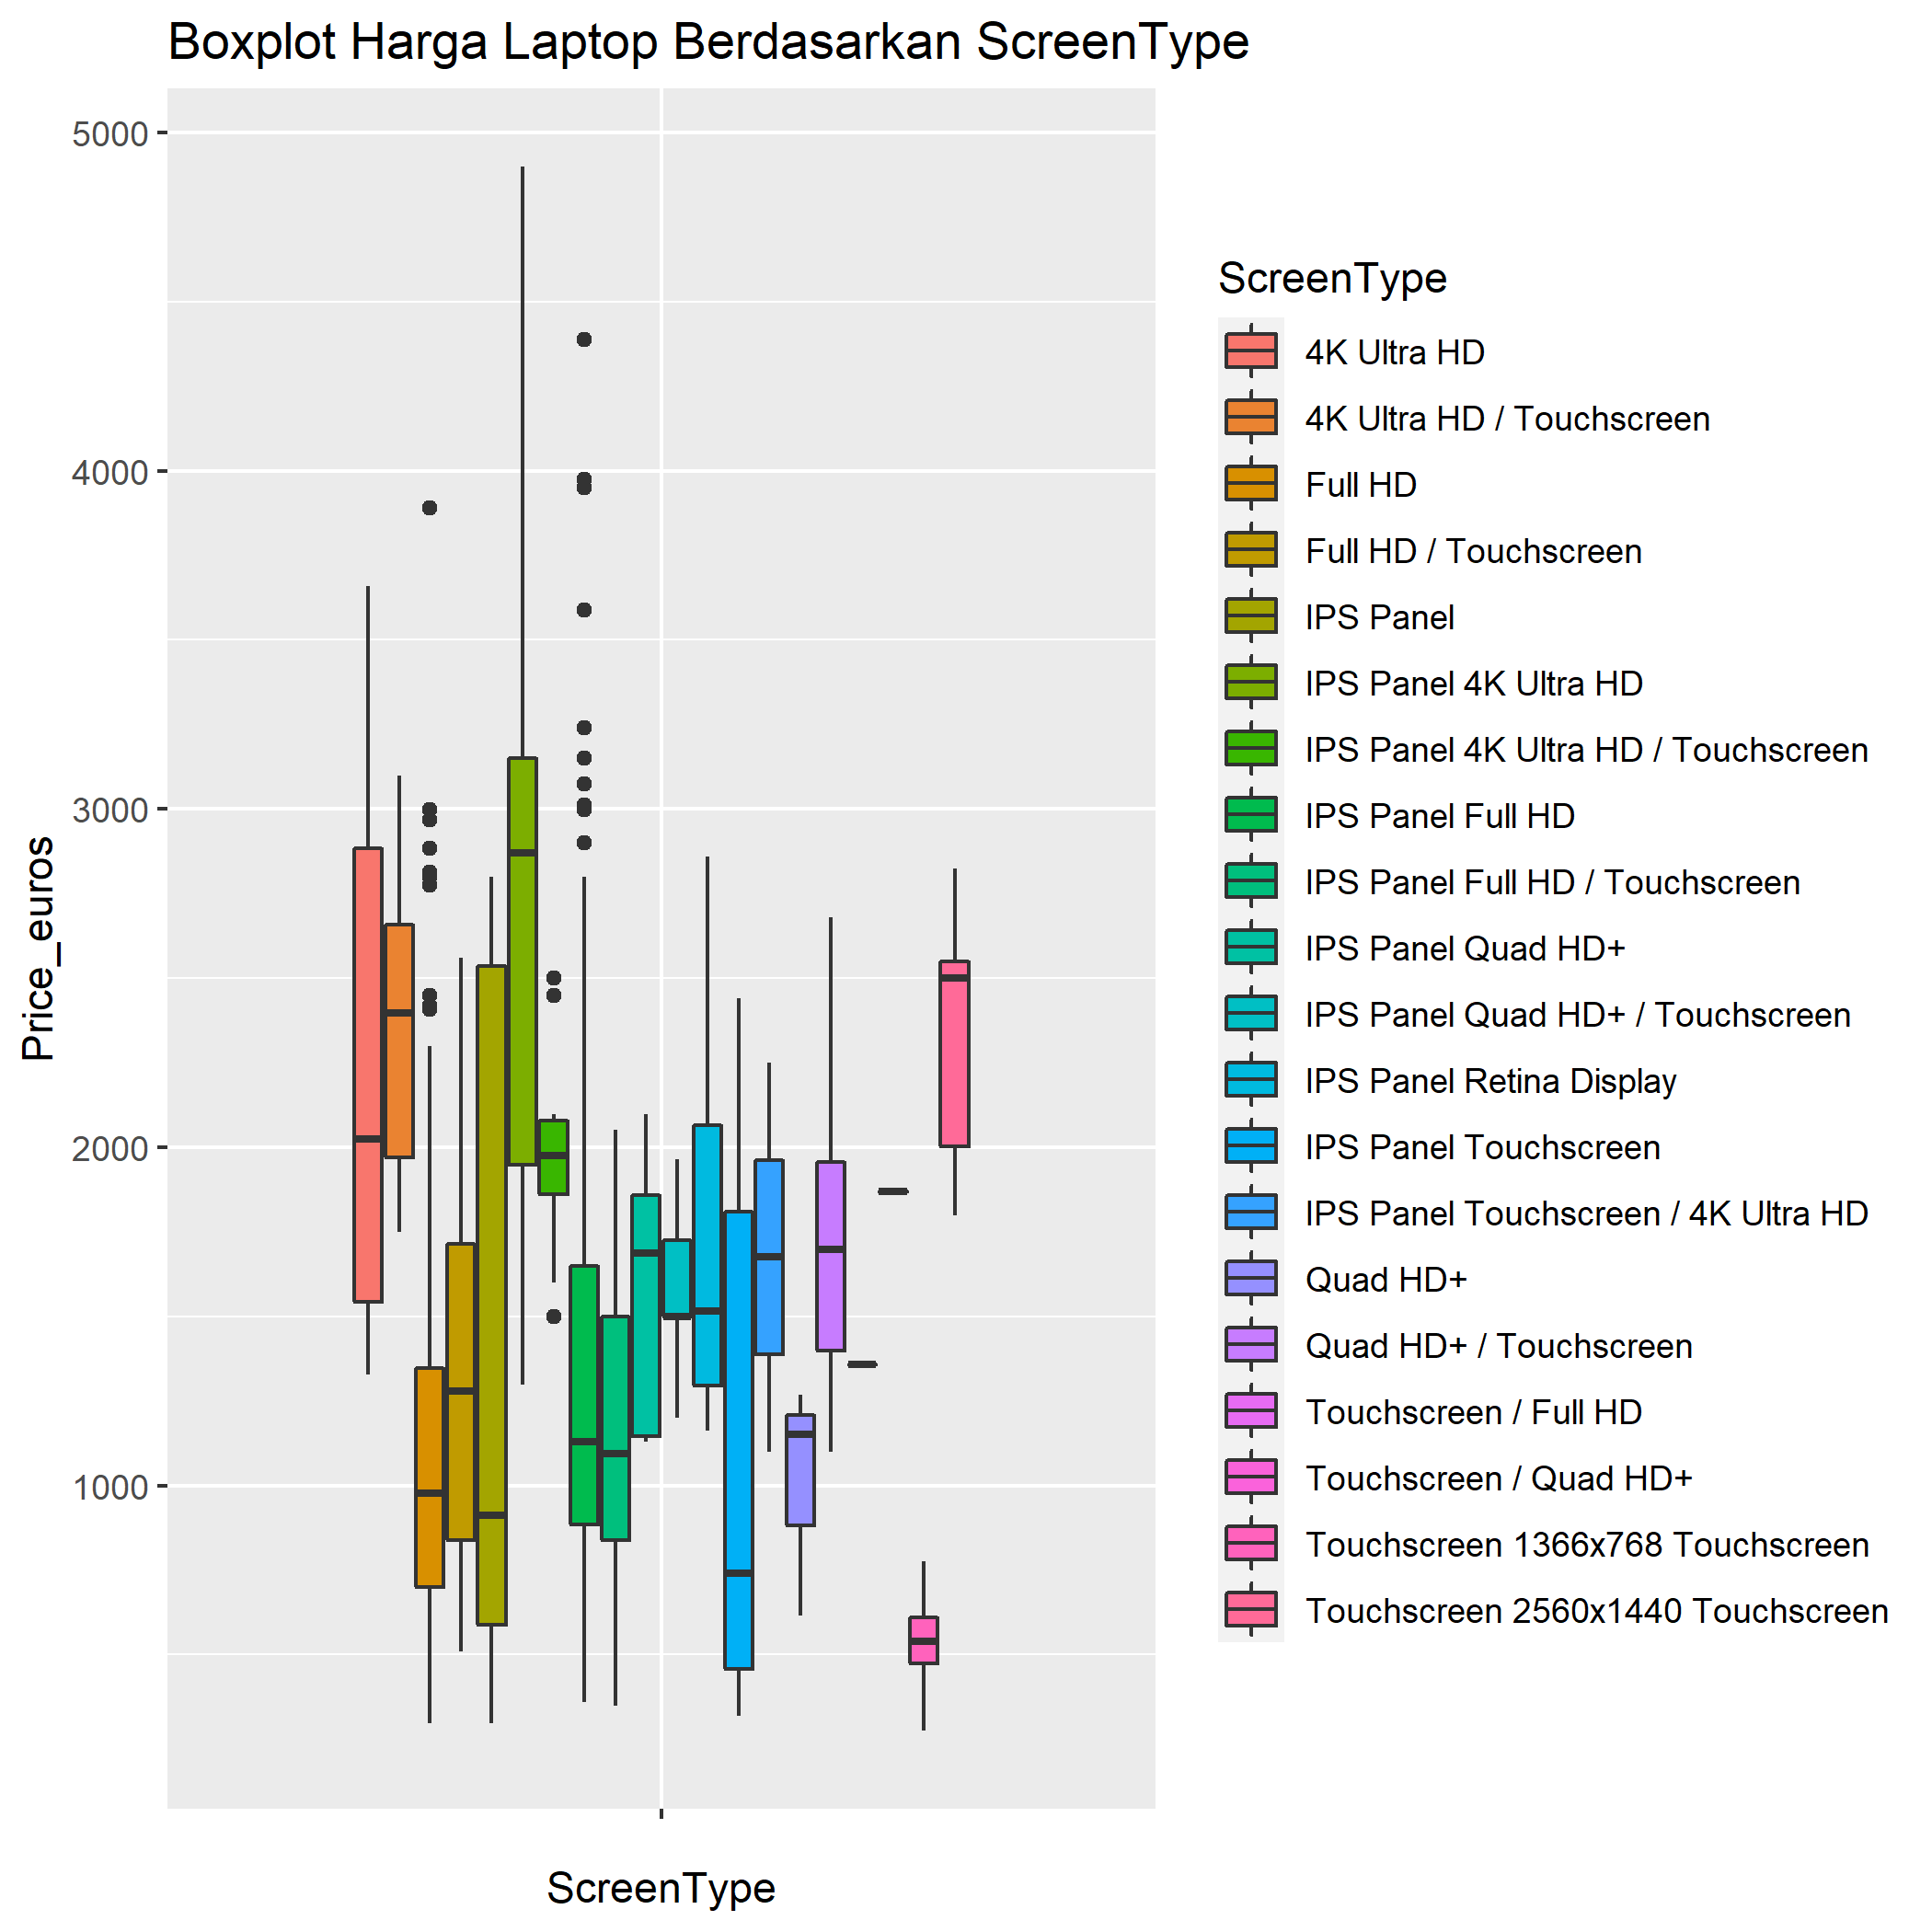
\includegraphics[scale = 0.4]{boxplot_price2.png}
    \caption{Diagram Kotak Garis Harga Berdasarkan ScreenType}
    \label{Resol}
\end{figure}  
  
\subsubsection{Hubungan antara Harga Laptop dengan Cpu\_Type dan Gpu\_Type}
Jika ditinjau dari Cpu\_Type dan Gpu\_Typenya dapat dilihat dari gambar Diagram Kotak Garis di bawah ini bahwa tipe AMD memiliki range dan harga yang paling murah dibandingkan yang lain dengan Tipe CPU Intel dan GPU Nvidia yang memiliki range yang paling besar dan harga yang paling mahal.   
  
\begin{figure}[h!]
    \centering
    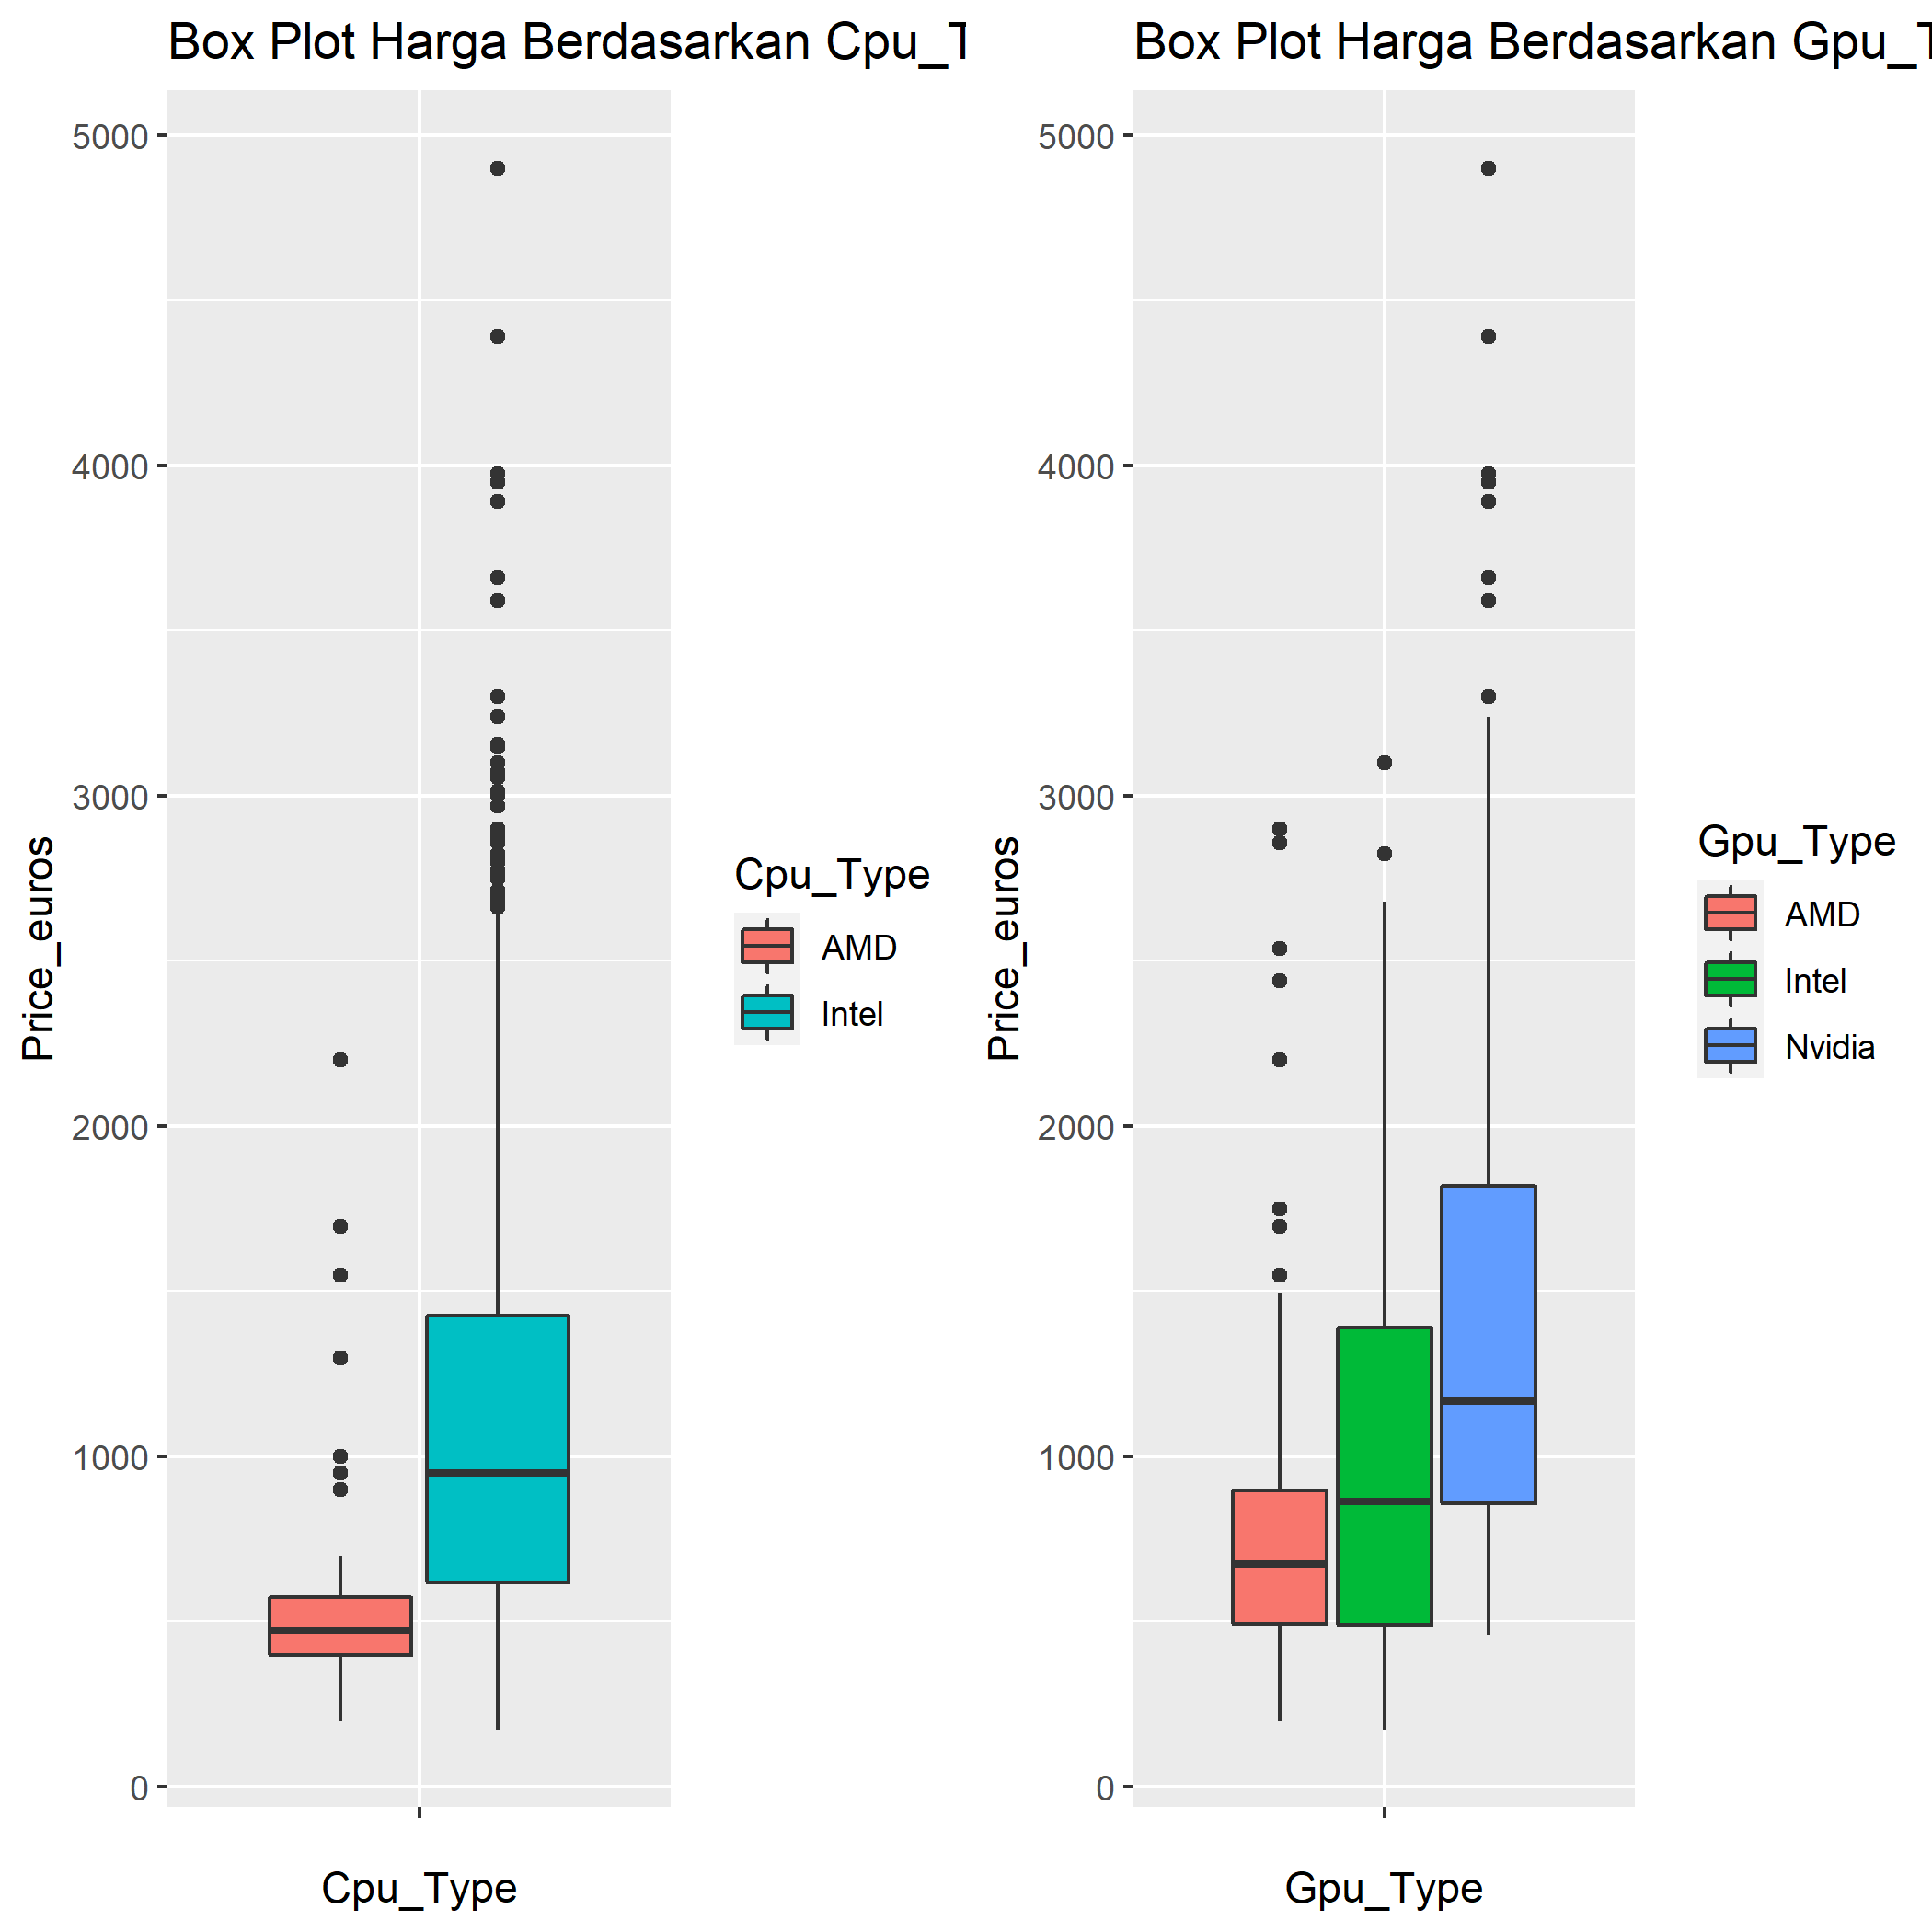
\includegraphics[scale = 0.4]{boxplot_price3.png}
    \caption{Diagram Kotak Garis Harga Berdasarkan Cpu\_Type dan Gpu\_Type}
    \label{Resol}
\end{figure}  

\subsubsection{Hubungan antara Harga Laptop dengan Memory\_1\_Size dan Memory\_2\_Size}
Jika ditinjau dari Memory\_1\_Size dan Memory\_2\_Size dapat dilihat dari diagram pencar di bawah ini bahwa tidak semua laptop dengan ukuran memori yang tinggi memiliki harga yang mahal.   

  
\begin{figure}[h!]
    \centering
    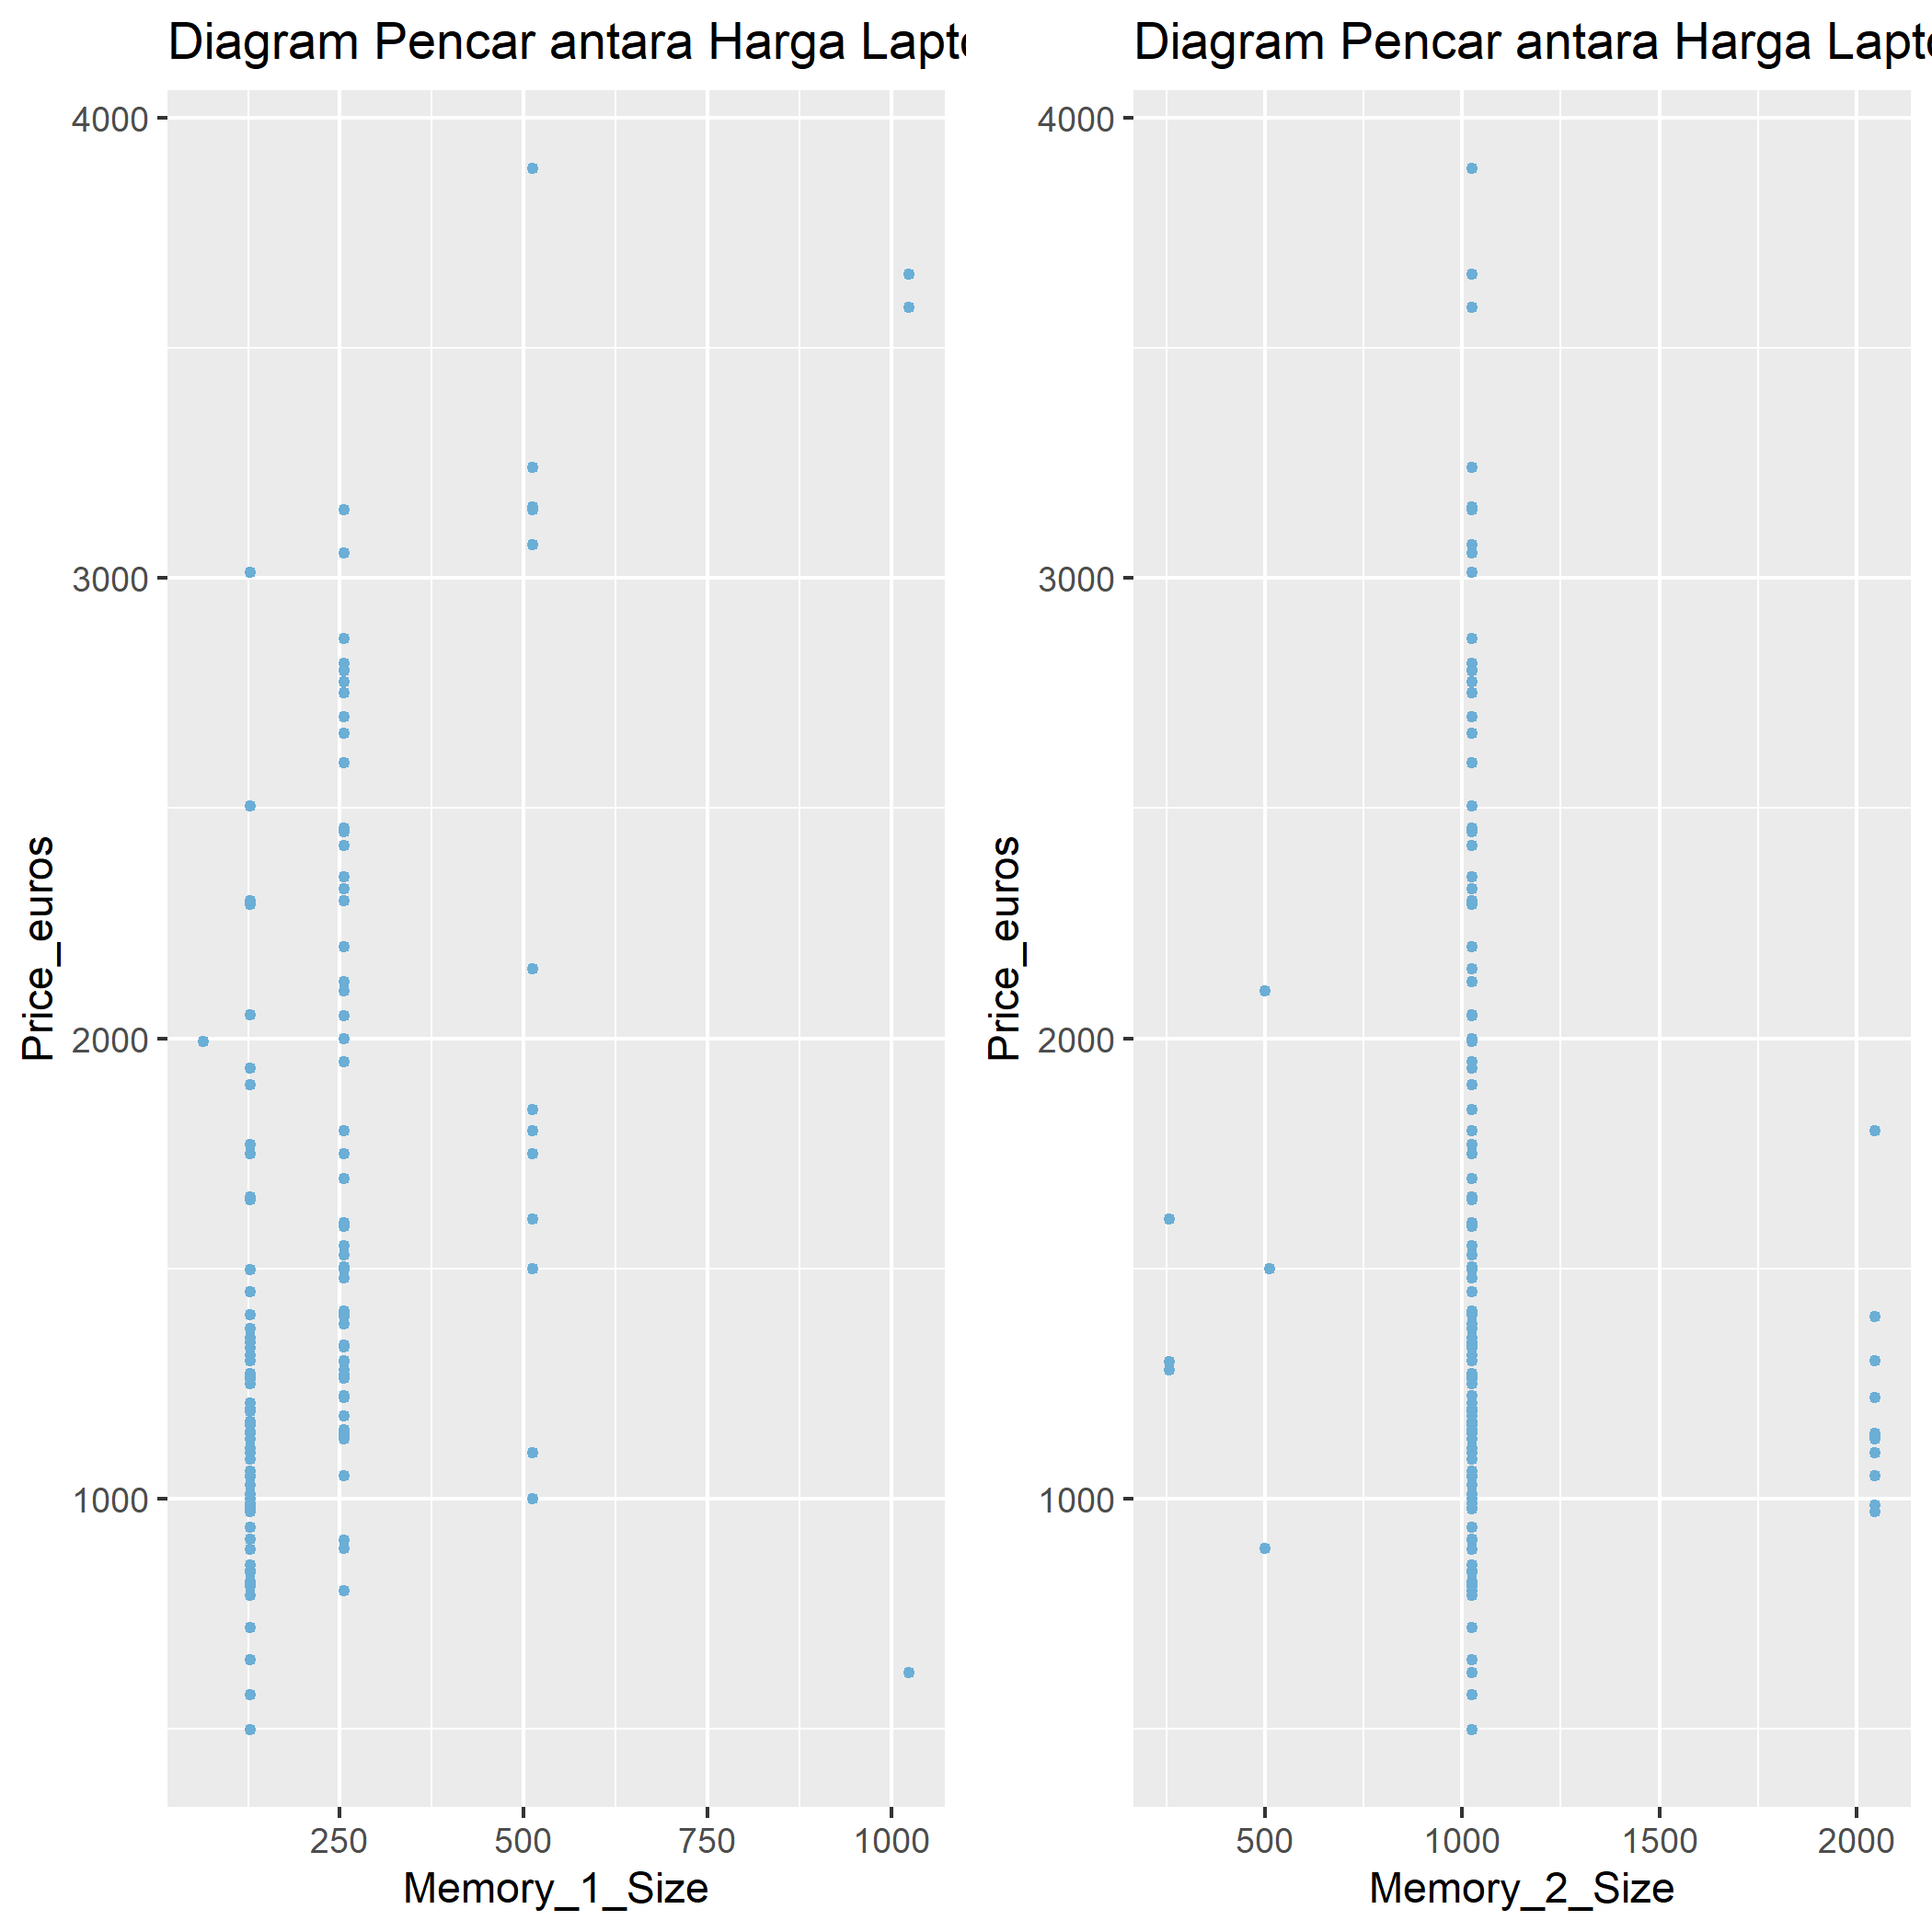
\includegraphics[scale = 0.4]{scatter_price0.png}
    \caption{Diagram Pencar Harga Berdasarkan Memory\_1\_Size dan Memory\_2\_Size}
    \label{Resol}
\end{figure}

\subsubsection{Interaksi}
Pada bagian ini akan dianalisis lebih lanjut mengenai hubungan antar kolom. Dapat dilihat pada diagram batang dibawah ini bahwa tidak semua perusahaan memiliki semua tipe laptop. Hal ini dapat menjadi salah satu pertimbangan untuk permodelan nantinya kolom Company dan TypeName harus saling berinteraksi agar ada batasan mengenai kombinasi antara nama perusahaan dengan tipe laptop yang dijual.    
  
\begin{figure}[h!]
    \centering
    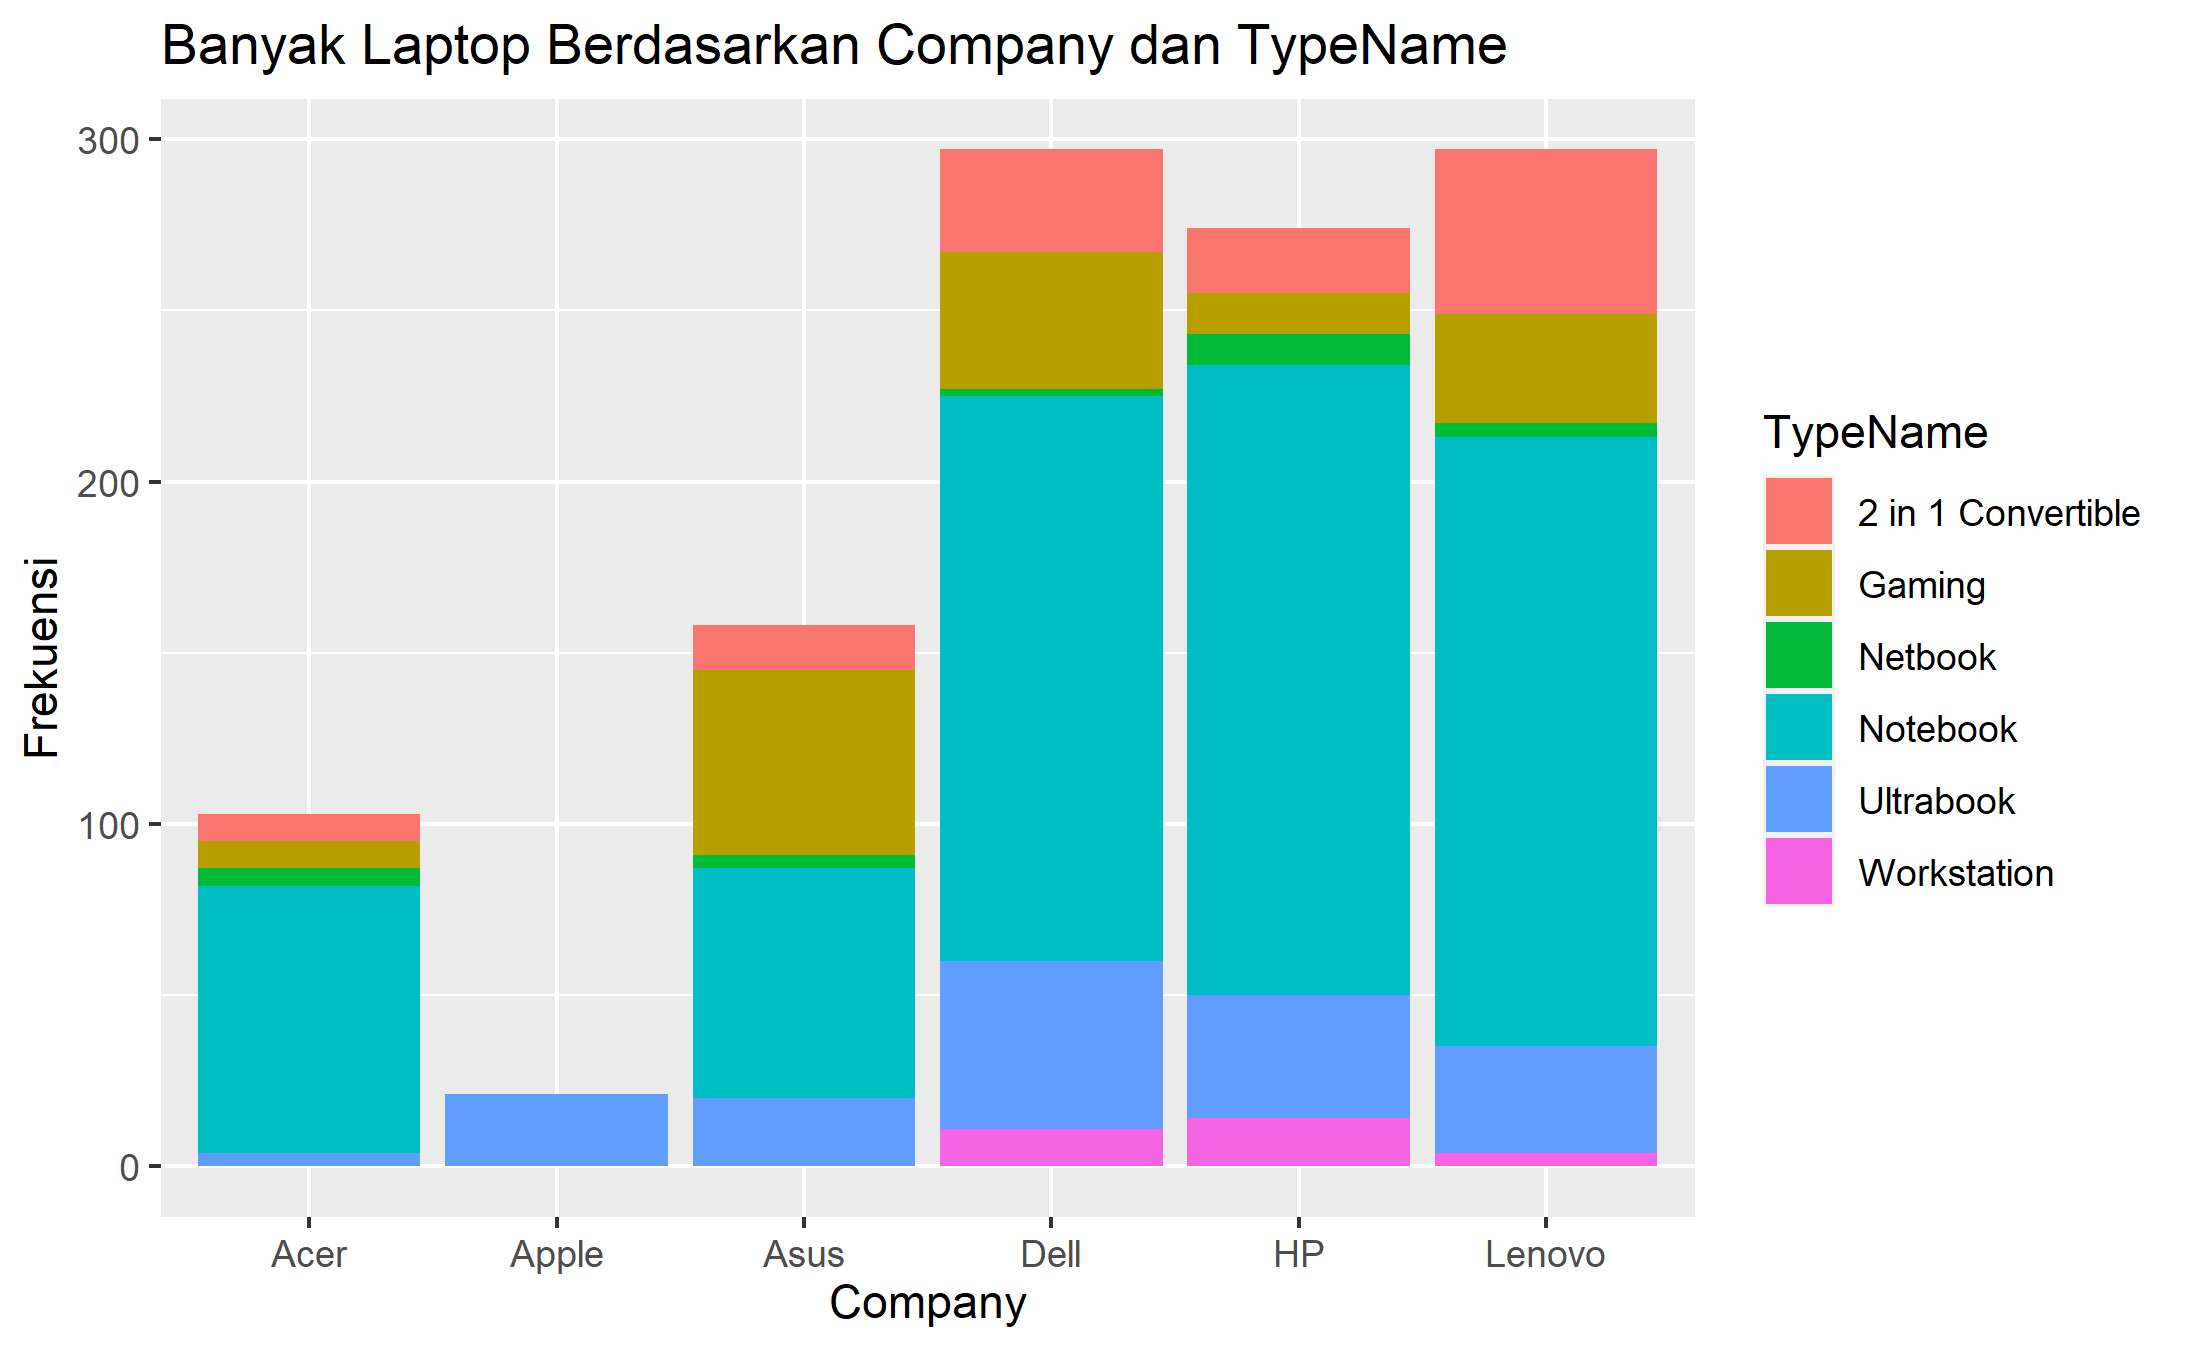
\includegraphics[scale = 0.4]{barplot_inter1.png}
    \caption{Diagram Batang Berdasarkan Company dan TypeName}
    \label{asdahay}
\end{figure}    
Begitu pula dengan OpSys, dapat dilihat bahwa perusahaan Apple memiliki \textit{Operating system} yang berbeda dengan perusahaan yang lain.   
  
\begin{figure}[h!]
    \centering
    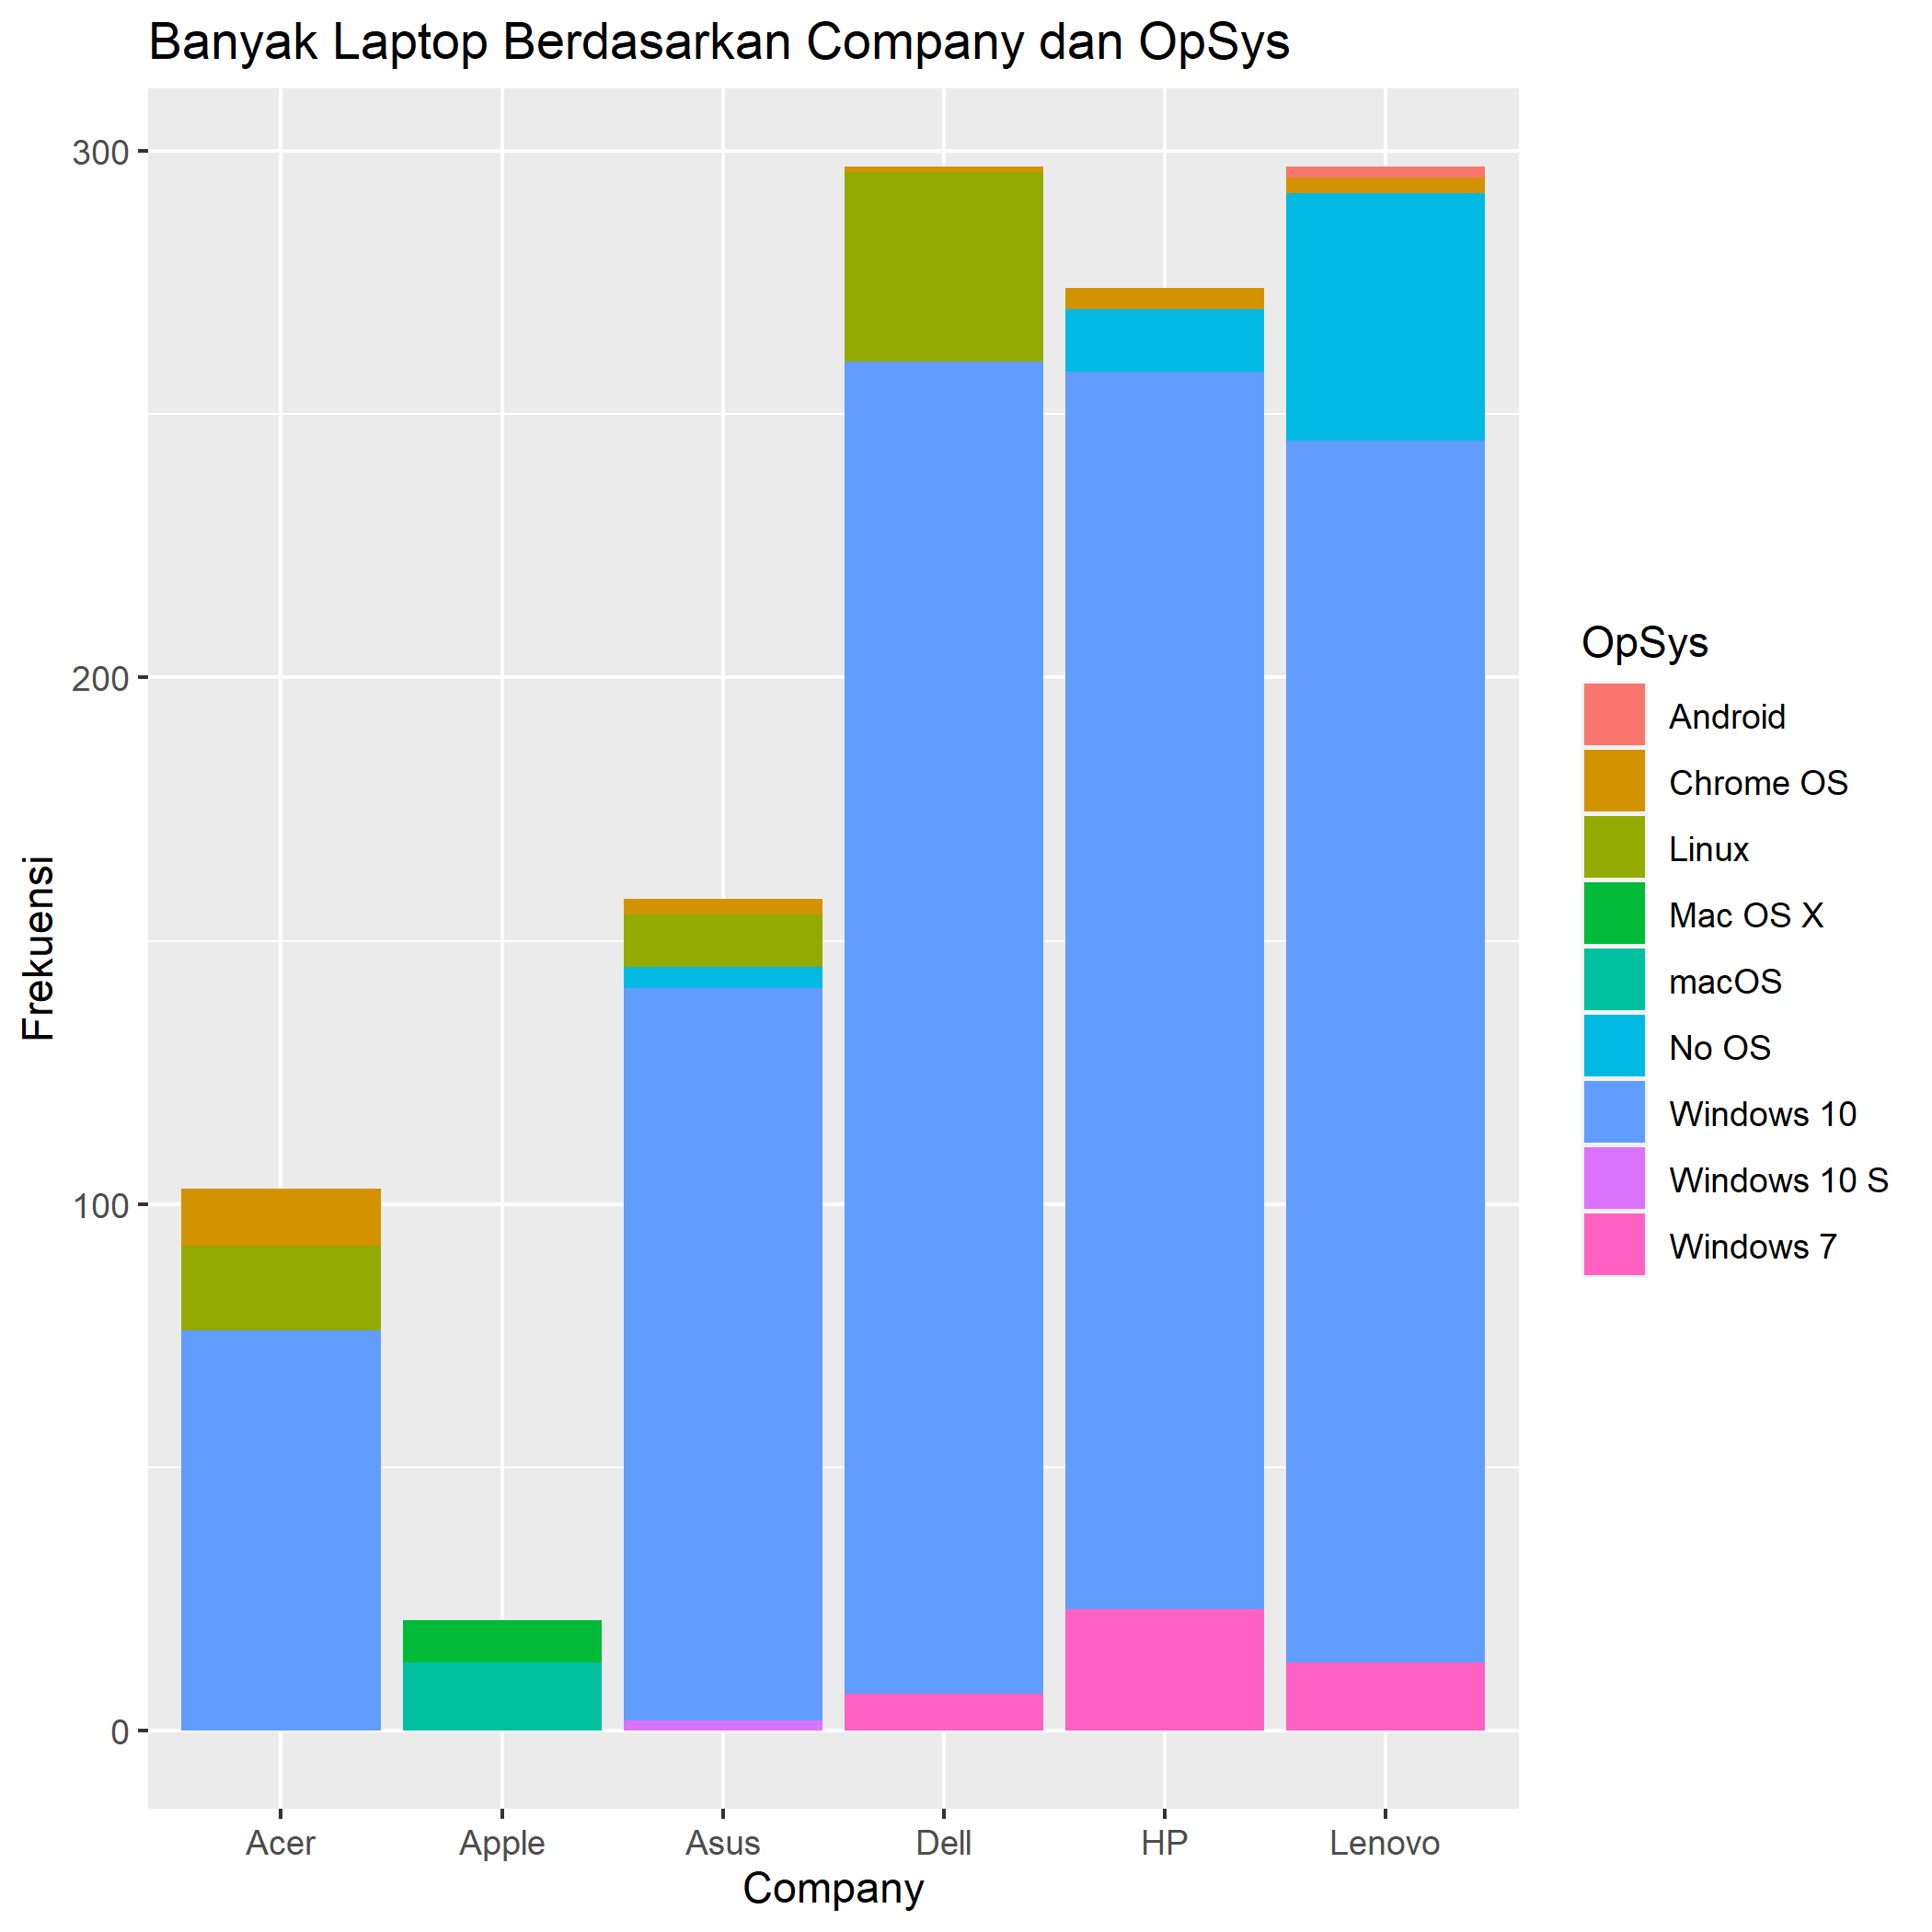
\includegraphics[scale = 0.4]{interaction2.png}
    \caption{Diagram Batang Berdasarkan Company dan OpSys}
    \label{asdahay}
\end{figure}    
\subsubsection{Kolinearitas}  
Ada dugaan bahwa semakin berat suatu laptop maka ukuran dari laptop tersebut juga semakin besar. Diperoleh korelasi antar Inches dan Weight adalah sebesar 0.82 sehingga hanya akan dipilih salah satu dari kolom tersebut untuk digunakan dalam permodelan.  

\begin{figure}[h!]
    \centering
    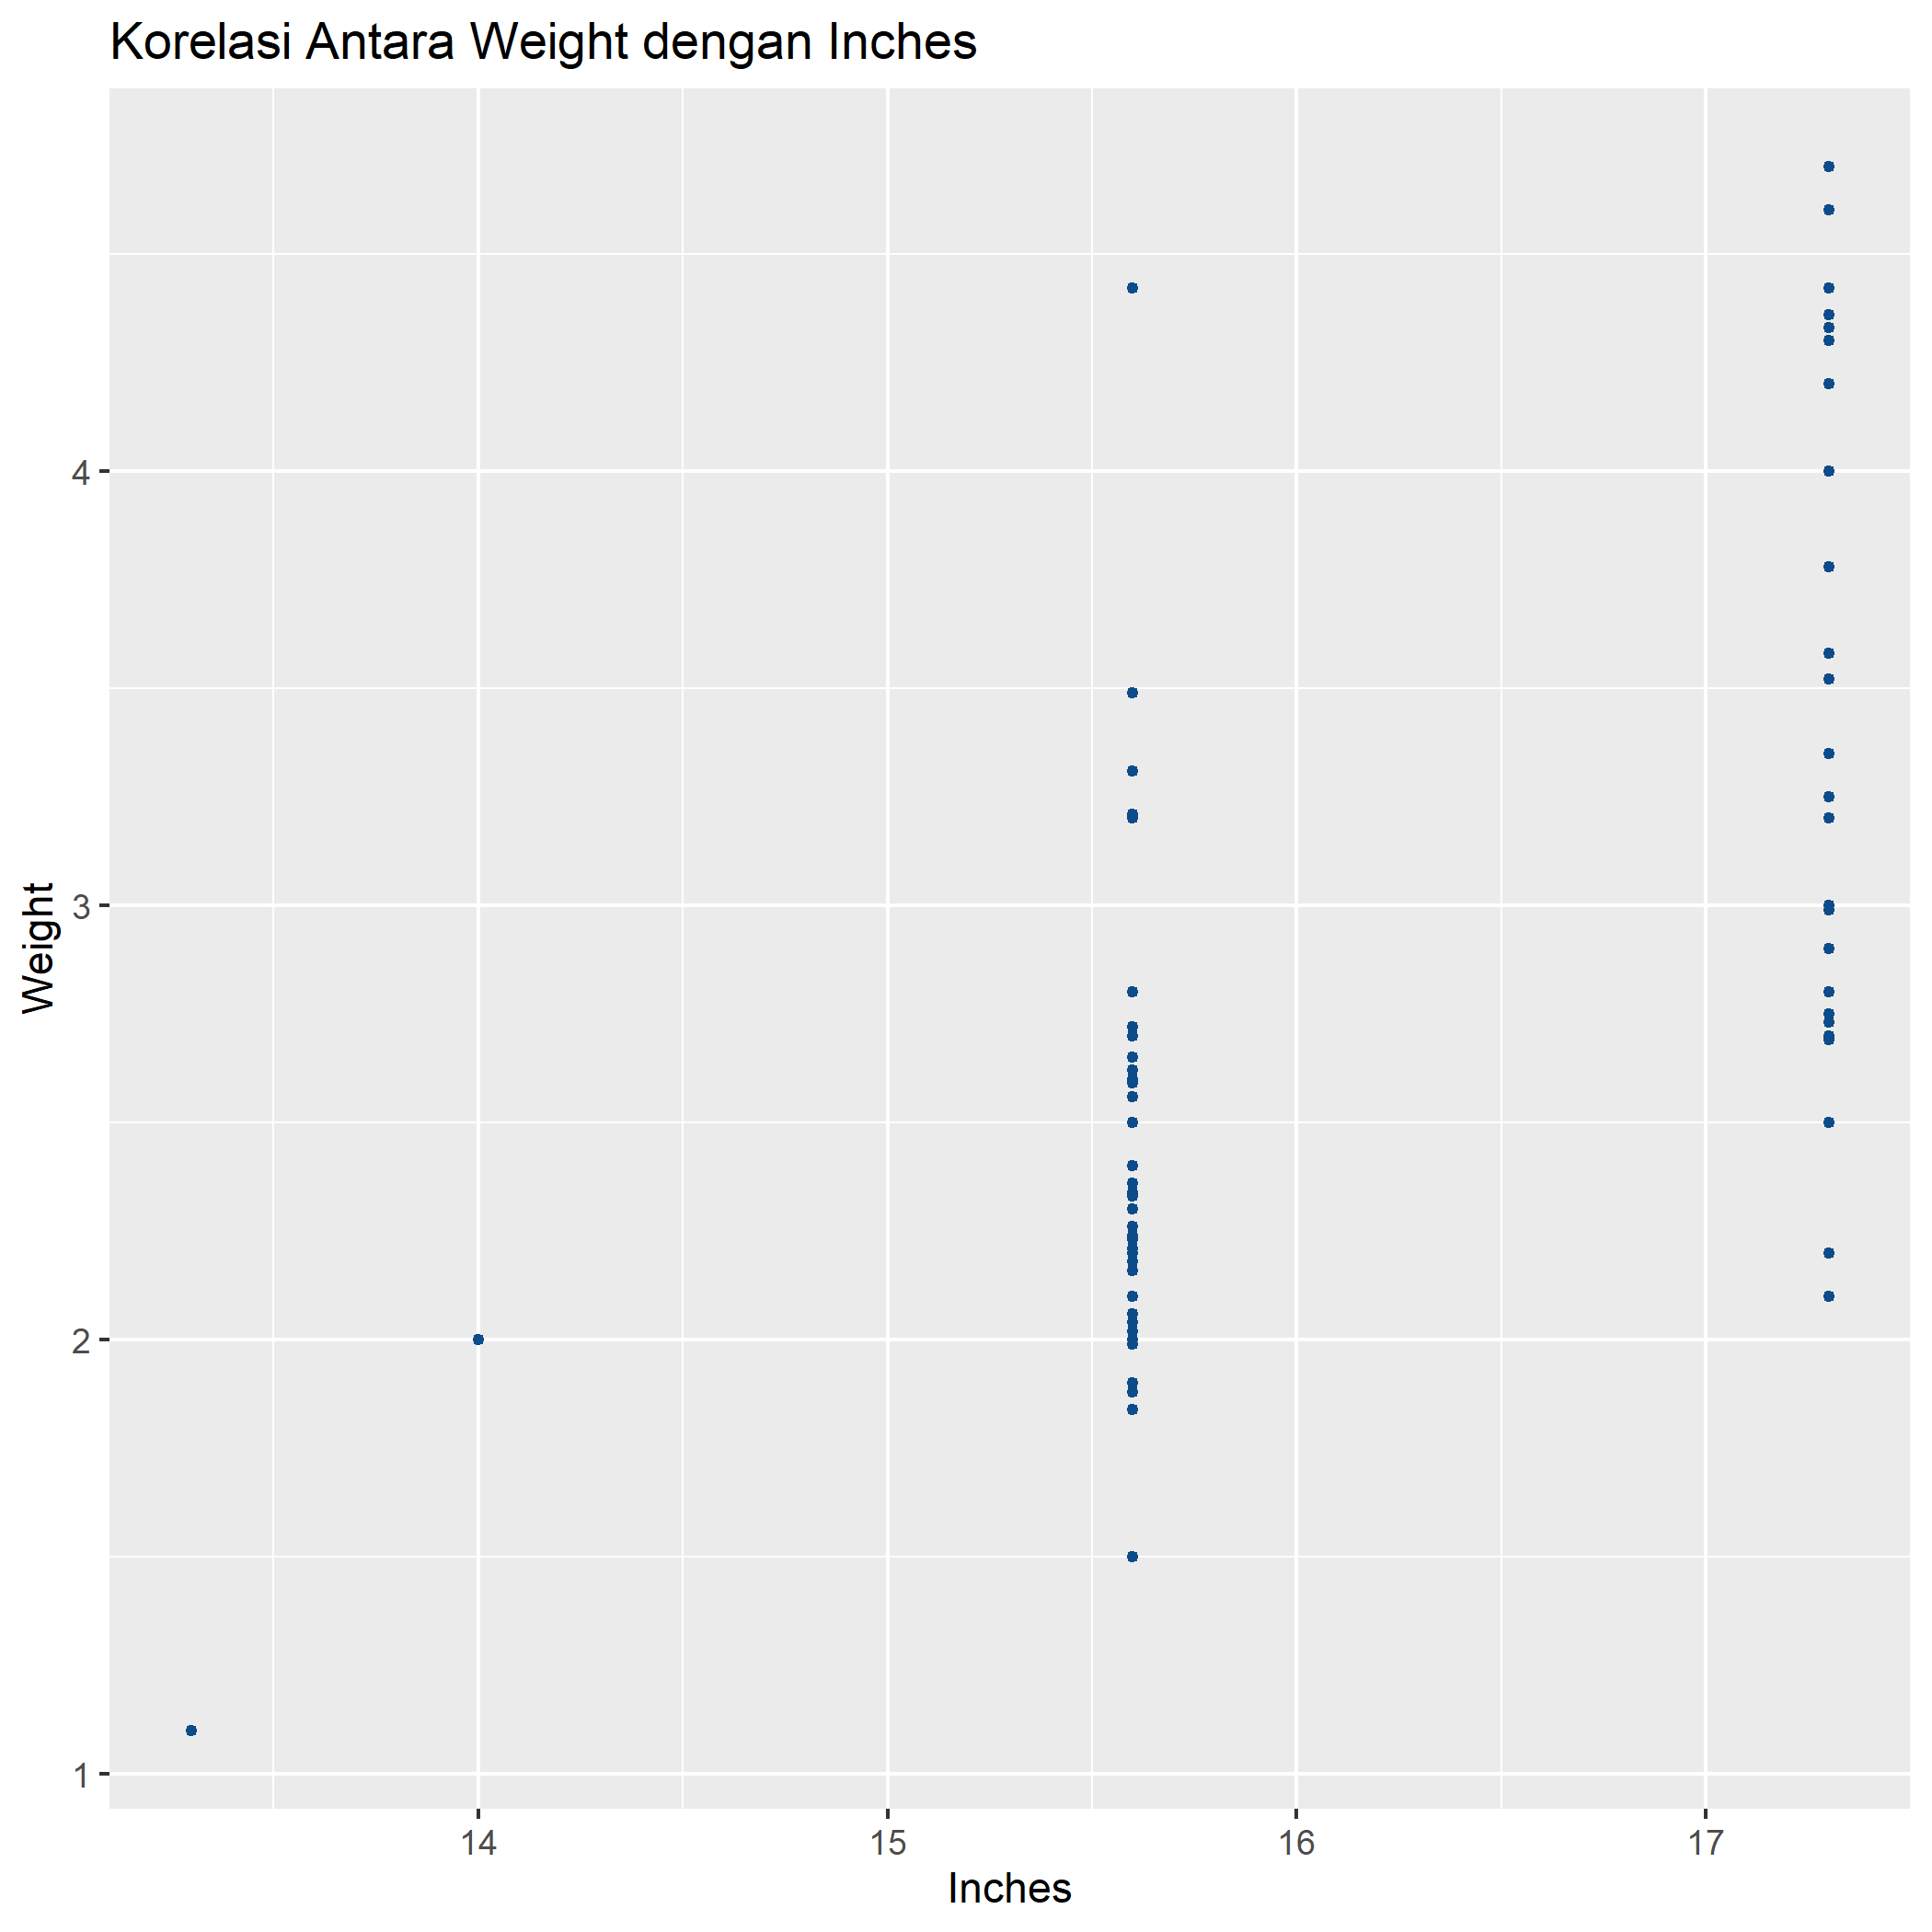
\includegraphics[scale = 0.4]{inchesweight.png}
    \caption{Diagram Pencar Antara Weight dengan Inches}
    \label{inches}
\end{figure}    

\subsection{Pengolahan Data / \textit{Data Processing}}
Sebelum membuat model, data akan dibagi menjadi 2 bagian yaitu bagian \textit{train} dan \textit{test} dengan \textit{train} memiliki 80\% dari data sepenuhnya dan 20\% untuk data \textit{test}.  
\par 
Berikutnya akan dipilih juga distribusi dari harga laptop. Akan dilakukan penaksiran parameter dari distribusi dan juga akan dilakukan uji Kolmogorov-Smirnov untuk menguji distribusi yang digunakan sudah sesuai. Dari data diperoleh rataan dari Harga Laptop adalah 1077.699 dengan variansi 444103.4.
\subsubsection{Harga Laptop Berdistribusi \textit{Gamma}}
Dengan bantuan piranti lunak R diperoleh taksiran untuk parameter distribusi \textit{Gamma} adalah $\hat{\mu} \approx 2.9281$ dan $\hat{\nu} \approx 42.934$. Jika diuji dengan Kolmogorov-Smirnov, diperoleh $p-\text{value}>\alpha$ sehingga dapat dikatakan bahwa distribusi dari harga laptop berdistribusi \textit{Gamma} dengan parameter $\hat{\mu} \approx 2.9281$ dan $\hat{\nu} \approx 42.934$.   
\begin{figure}[h!]
    \centering
    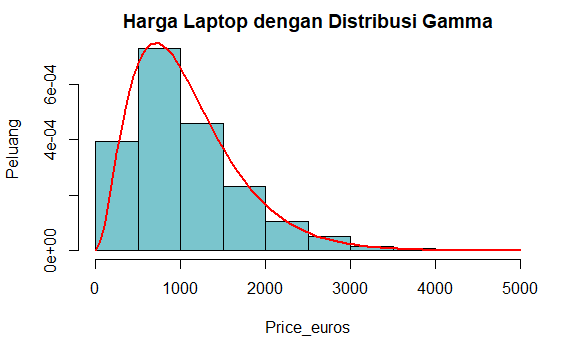
\includegraphics[scale = 0.5]{distg.png}
    \caption{Histogram dari Harga Laptop dengan Distribusi \textit{Gamma}}
    \label{fig:ashi}
\end{figure}  

\subsubsection{Harga Laptop Berdistribusi \textit{Inverse Gaussian}}
Dengan bantuan piranti lunak R diperoleh taksiran untuk parameter distribusi \textit{Inverse Gaussian} adalah $\hat{\mu} \approx 1077.730$ dan $\hat{\sigma}^2 \approx 2433.434$. Jika diuji dengan Kolmogorov-Smirnov, diperoleh $p-\text{value}>\alpha$ sehingga dapat dikatakan bahwa distribusi dari harga laptop berdistribusi \textit{Inverse Gaussian} dengan parameter $\hat{\mu} \approx 1077.730$ dan $\hat{\sigma}^2 \approx 2433.434$.
   
 \begin{figure}[h!]
    \centering
    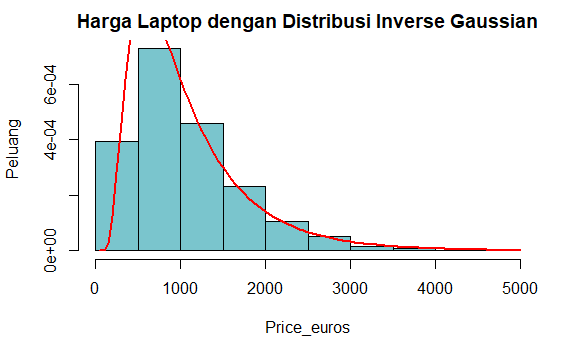
\includegraphics[scale = 0.5]{distinv.png}
    \caption{Histogram dari Harga Laptop dengan Distribusi \textit{Inverse Gaussian}}
    \label{fig:ashis}
\end{figure}  

\subsection{Permodelan Data / \textit{Data Modelling}}  
Permodelan data akan dilakukan sebanyak 2 kali dengan metode yang berbeda. Metode pertama adalah dengan memasukkan semua kolom yang ada (dinamakan model 1) tanpa ada interaksi dan model kedua adalah model dengan kolom-kolom pilihan yaitu kolom Company, TypeName, Inches, ScreenResolution, Cpu\_Type, Ram, Memory\_1\_Size, Memory\_1\_Type, Gpu\_Type, dan OpSys dengan melibatkan interaksi antar Company dan OpSys. Kedua model ini akan menggunakan \textit{link function} log. Dan pemilihan model menggunakan metode \textit{Stepwise Regression} yang akan dibantu dengan piranti lunak R.  
\subsubsection{Model Pertama} 
Dengan distribusi \textit{Gamma} diperoleh kolom-kolom yang ada dalam model adalah kolom Company, TypeName, Inches, ScreenResolution, Cpu\_Series, Ram, Memory\_1\_Type, Memory\_2\_Type, Gpu\_Series dan OpSys. Terdapat 204 parameter pada model pertama dengan distribusi \textit{Gamma} dengan 18 parameter yang singular. Hal ini bisa disebabkan karna data dengan karakteristik tersebut hanya berjumlah 1. Sehingga diperoleh suatu persamaan :
\begin{equation}
    \label{Gamma_eq}
    \mu_{1,\text{Gamma}} = \exp{\left(7.288479+\sum_{i=1}^8x_i -0.039716x_9+0.022645x_{10}\right)}
\end{equation}  
Dengan $x_1, \dots x_8$ adalah suatu fungsi indikator untuk kolom-kolom factor dengan koefisiennya masing-masing. Karena keterbatasan tempat maka tidak ditulis secara penuh dan akan dilampirkan keluaran dari piranti lunak R di bagian Appendix \ref{Model_1_Gamma}. $x_9$ adalah Inches dan $x_{10}$ adalah Ram. 
Dan \textit{deviance} dari model pertama dengan distribusi \textit{Gamma} adalah 31.22367. 
\par 
Sedangkan untuk distribusi \textit{Inverse Gaussian} diperoleh kolom-kolom yang ada dalam model adalah kolom Company, TypeName, Inches, ScreenResolution, ScreenType, Cpu\_Series, Ram, Memory\_1\_Type, Memory\_2\_Size, dan OpSys. Terdapat 134 parameter dengan 8 parameter yang singular. Sehingga diperoleh suatu persamaan :
\begin{equation}
    \label{Gamma_eq}
    \mu_{1,\text{Inv}} = \exp{\left(7.030+\sum_{i=1}^7x_i-0.0307x_8+0.03164x_9+0.0000522x_{10}\right)}
\end{equation}  
Dengan $x_1, \dots x_7$ adalah suatu fungsi indikator untuk kolom-kolom factor dengan koefisiennya masing-masing. Karena keterbatasan tempat maka tidak ditulis secara penuh dan akan dilampirkan keluaran dari piranti lunak R di bagian Appendix \ref{Model_1_Inv}. $x_8$ adalah Inches, $x_9$ adalah Ram dan $x_{10}$ adalah Memory\_2\_Size. 
Dan \textit{deviance} dari model pertama dengan distribusi \textit{Inverse Gaussian} adalah 0.04274252. 
\par
Jika kedua model diuji dengan data \textit{train} maka model dengan distribusi \textit{Gamma} memiliki nilai MAPE sebesar 14.23\% dan model dengan distribusi \textit{Inverse Gaussian} memiliki nilai MAPE 16.55\%.  
\par 
Kedua model tidak dapat diuji dengan data \textit{test} karena ada beberapa data yang berada diluar parameter yang dimodelkan pada data \textit{train}. Hal ini disebabkan karena data dengan karakteristik tersebut hanya muncul 1 kali sehingga tidak masuk ke data \textit{train}.  
\par 
Dengan bantuan piranti lunak R dapat diperoleh suatu tabel \textit{Analysis of Deviance} untuk menentukan signifikan atau tidaknya suatu parameter dan diperoleh model pertama dengan distribusi \textit{Gamma} dan \textit{Inverse Gaussian}  diperoleh signifikan.
\subsubsection{Model Kedua}
Dengan distribusi \textit{Gamma} diperoleh kolom-kolom yang ada dalam model adalah kolom Company, TypeName, Inches, ScreenResolution, Cpu\_Type, Ram, Memory\_1\_Type, Gpu\_Type, OpSys dan Company$\times$TypeName. Terdapat 62 parameter pada model kedua dengan distribusi \textit{Gamma} dengan 8 parameter yang singular. Sehingga diperoleh suatu persamaan :
\begin{equation}
    \label{Gamma_eq2}
    \mu_{2,\text{Gamma}} = \exp{\left(7.1010246+\sum_{i=1}^8x_i -0.0333378x_9+0.0457834x_{10}\right)}
\end{equation}  
Dengan $x_1, \dots x_8$ adalah suatu fungsi indikator untuk kolom-kolom \textit{factor} dengan koefisiennya masing-masing. Lebih lanjut $x_8=x_{\text{Company}}\times x_{\text{TypeName}}$. Karena keterbatasan tempat maka tidak ditulis secara penuh dan akan dilampirkan keluaran dari piranti lunak R di bagian Appendix \ref{Model_2_Gamma}. $x_9$ adalah Inches,dan $x_{10}$ adalah Ram.  Dan \textit{deviance} dari model kedua dengan distribusi \textit{Gamma} adalah 67.751.
\par 
Sedangkan untuk distribusi \textit{Inverse Gaussian} diperoleh kolom-kolom yang ada dalam model adalah kolom Company, TypeName, Inches, ScreenResolution, Cpu\_Type, Ram, Memory\_1\_Type, Gpu\_Type, OpSys, Company$\times$OpSys dan Company$\times$TypeName .  Sehingga diperoleh suatu persamaan :
\begin{equation}
    \label{Inv_eq2}
    \mu_{2,\text{Inv}} = \exp{\left(7.240570+\sum_{i=1}^{10}x_i -0.052403x_{11}+0.060701x_{12}\right)}
\end{equation} 
Dengan $x_1, \dots x_8$ adalah suatu fungsi indikator untuk kolom-kolom \textit{factor} dengan koefisiennya masing-masing. Lebih lanjut, $x_9 = x_{\text{Company}}\times x_{\text{OpSys}}$ dan $x_{10} = x_{\text{Company}}\times x_{\text{TypeName}}$. Karena keterbatasan tempat maka tidak ditulis secara penuh dan akan dilampirkan keluaran dari piranti lunak R di bagian Appendix \ref{Model_2_Inv}. $x_{11}$ adalah Inches,dan $x_{12}$ adalah Ram. Terdapat 133 parameter dengan 38 parameter yang singular. Dan \textit{deviance} dari model kedua dengan distribusi \textit{Inverse Gaussian} adalah 0.081343. 
\par
Jika kedua model diuji dengan data \textit{train} maka model dengan distribusi \textit{Gamma} memiliki nilai MAPE sebesar 22.23\% dan pada data \textit{test} diperoleh nilai MAPE sebesar 23.02 dan model dengan distribusi \textit{Inverse Gaussian} memiliki nilai MAPE 26.56\%. dan pada data \textit{test} diperoleh nilai MAPE 30.65\%.    
\par
Dengan bantuan piranti lunak R dapat diperoleh suatu tabel \textit{Analysis of Deviance} dan diperoleh model kedua dengan distribusi \textit{Gamma} diperoleh signifikan dan model kedua dengan distribusi \textit{Inverse Gaussian} diperoleh parameter untuk Company:OpSys tidak signifikan.
\subsection{Analisis Residu}  
Seperti yang telah dijelaskan pada bagian Metodologi, akan dilihat ada atau tidaknya $|\delta_i|>1$ yang menunjukkan ketidakcocokkan model pada data. 
\par
Pada model pertama dapat dilihat bahwa  dari Distribusi \textit{Gamma} hanya ada 1 data yang lebih besar dari 1 sedangkan pada model \textit{Inverse Gaussian} ada 2 data yang lebih besar dari 1.
  
\begin{figure}[h!]
    \centering
    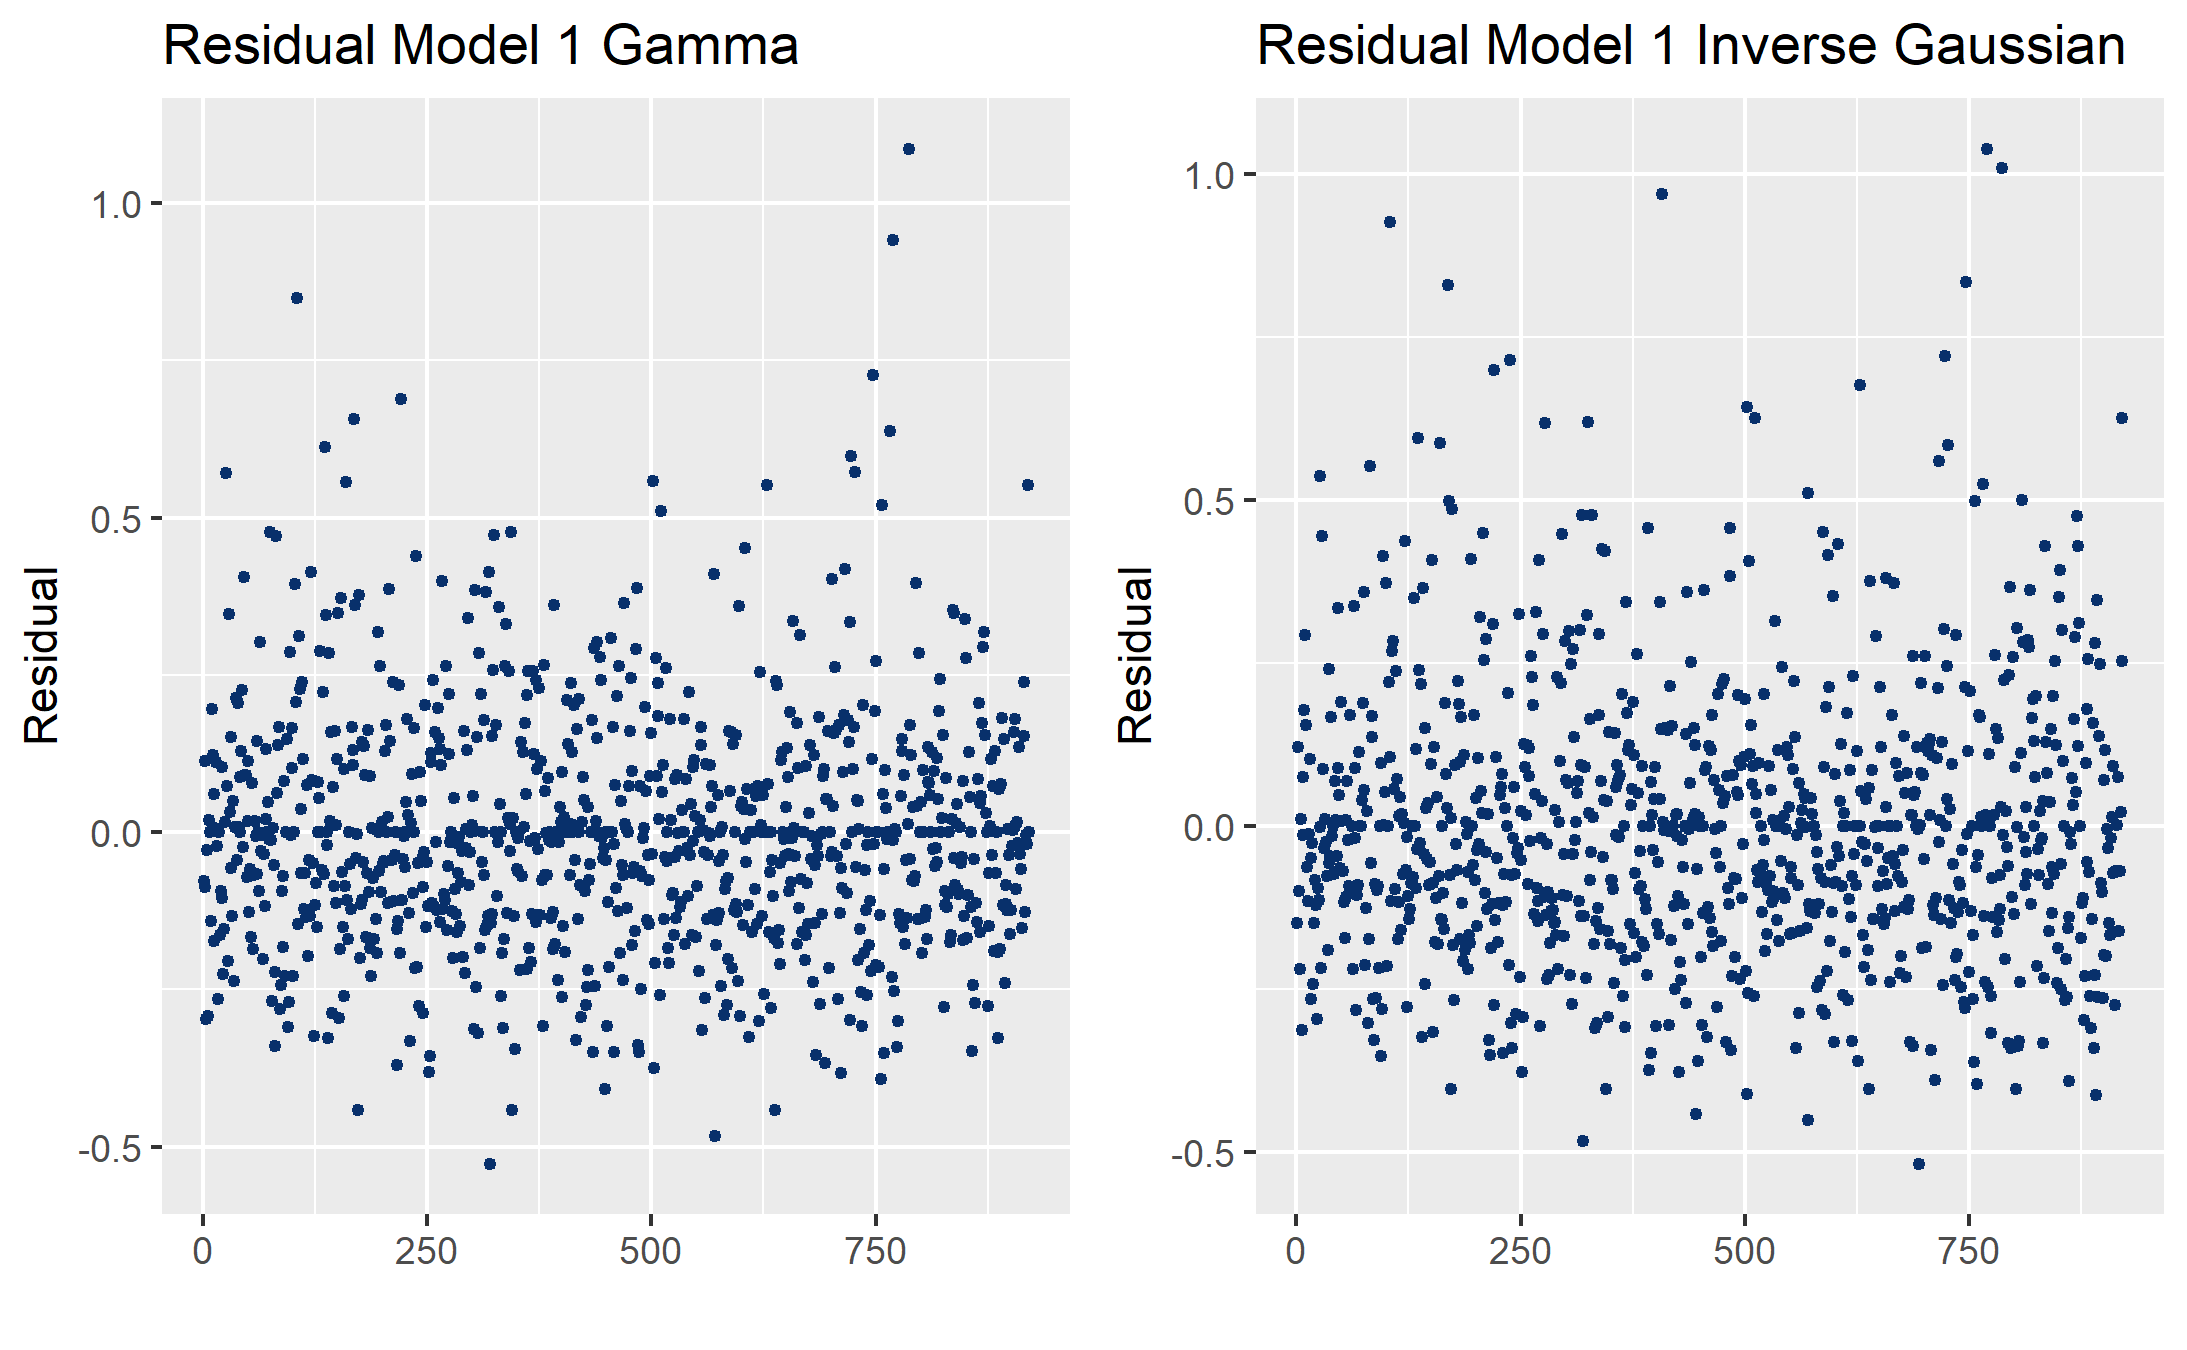
\includegraphics[scale = 0.4]{resid1.png}
    \caption{Residual dari Model Pertama}
    \label{fig:resifddd}
\end{figure}    
    
Sedangkan pada model kedua dapat dilihat bahwa data dengan residual $> 1$ jauh lebih banyak dibanding dengan model pertama.  
  
\begin{figure}[h!]
    \centering
    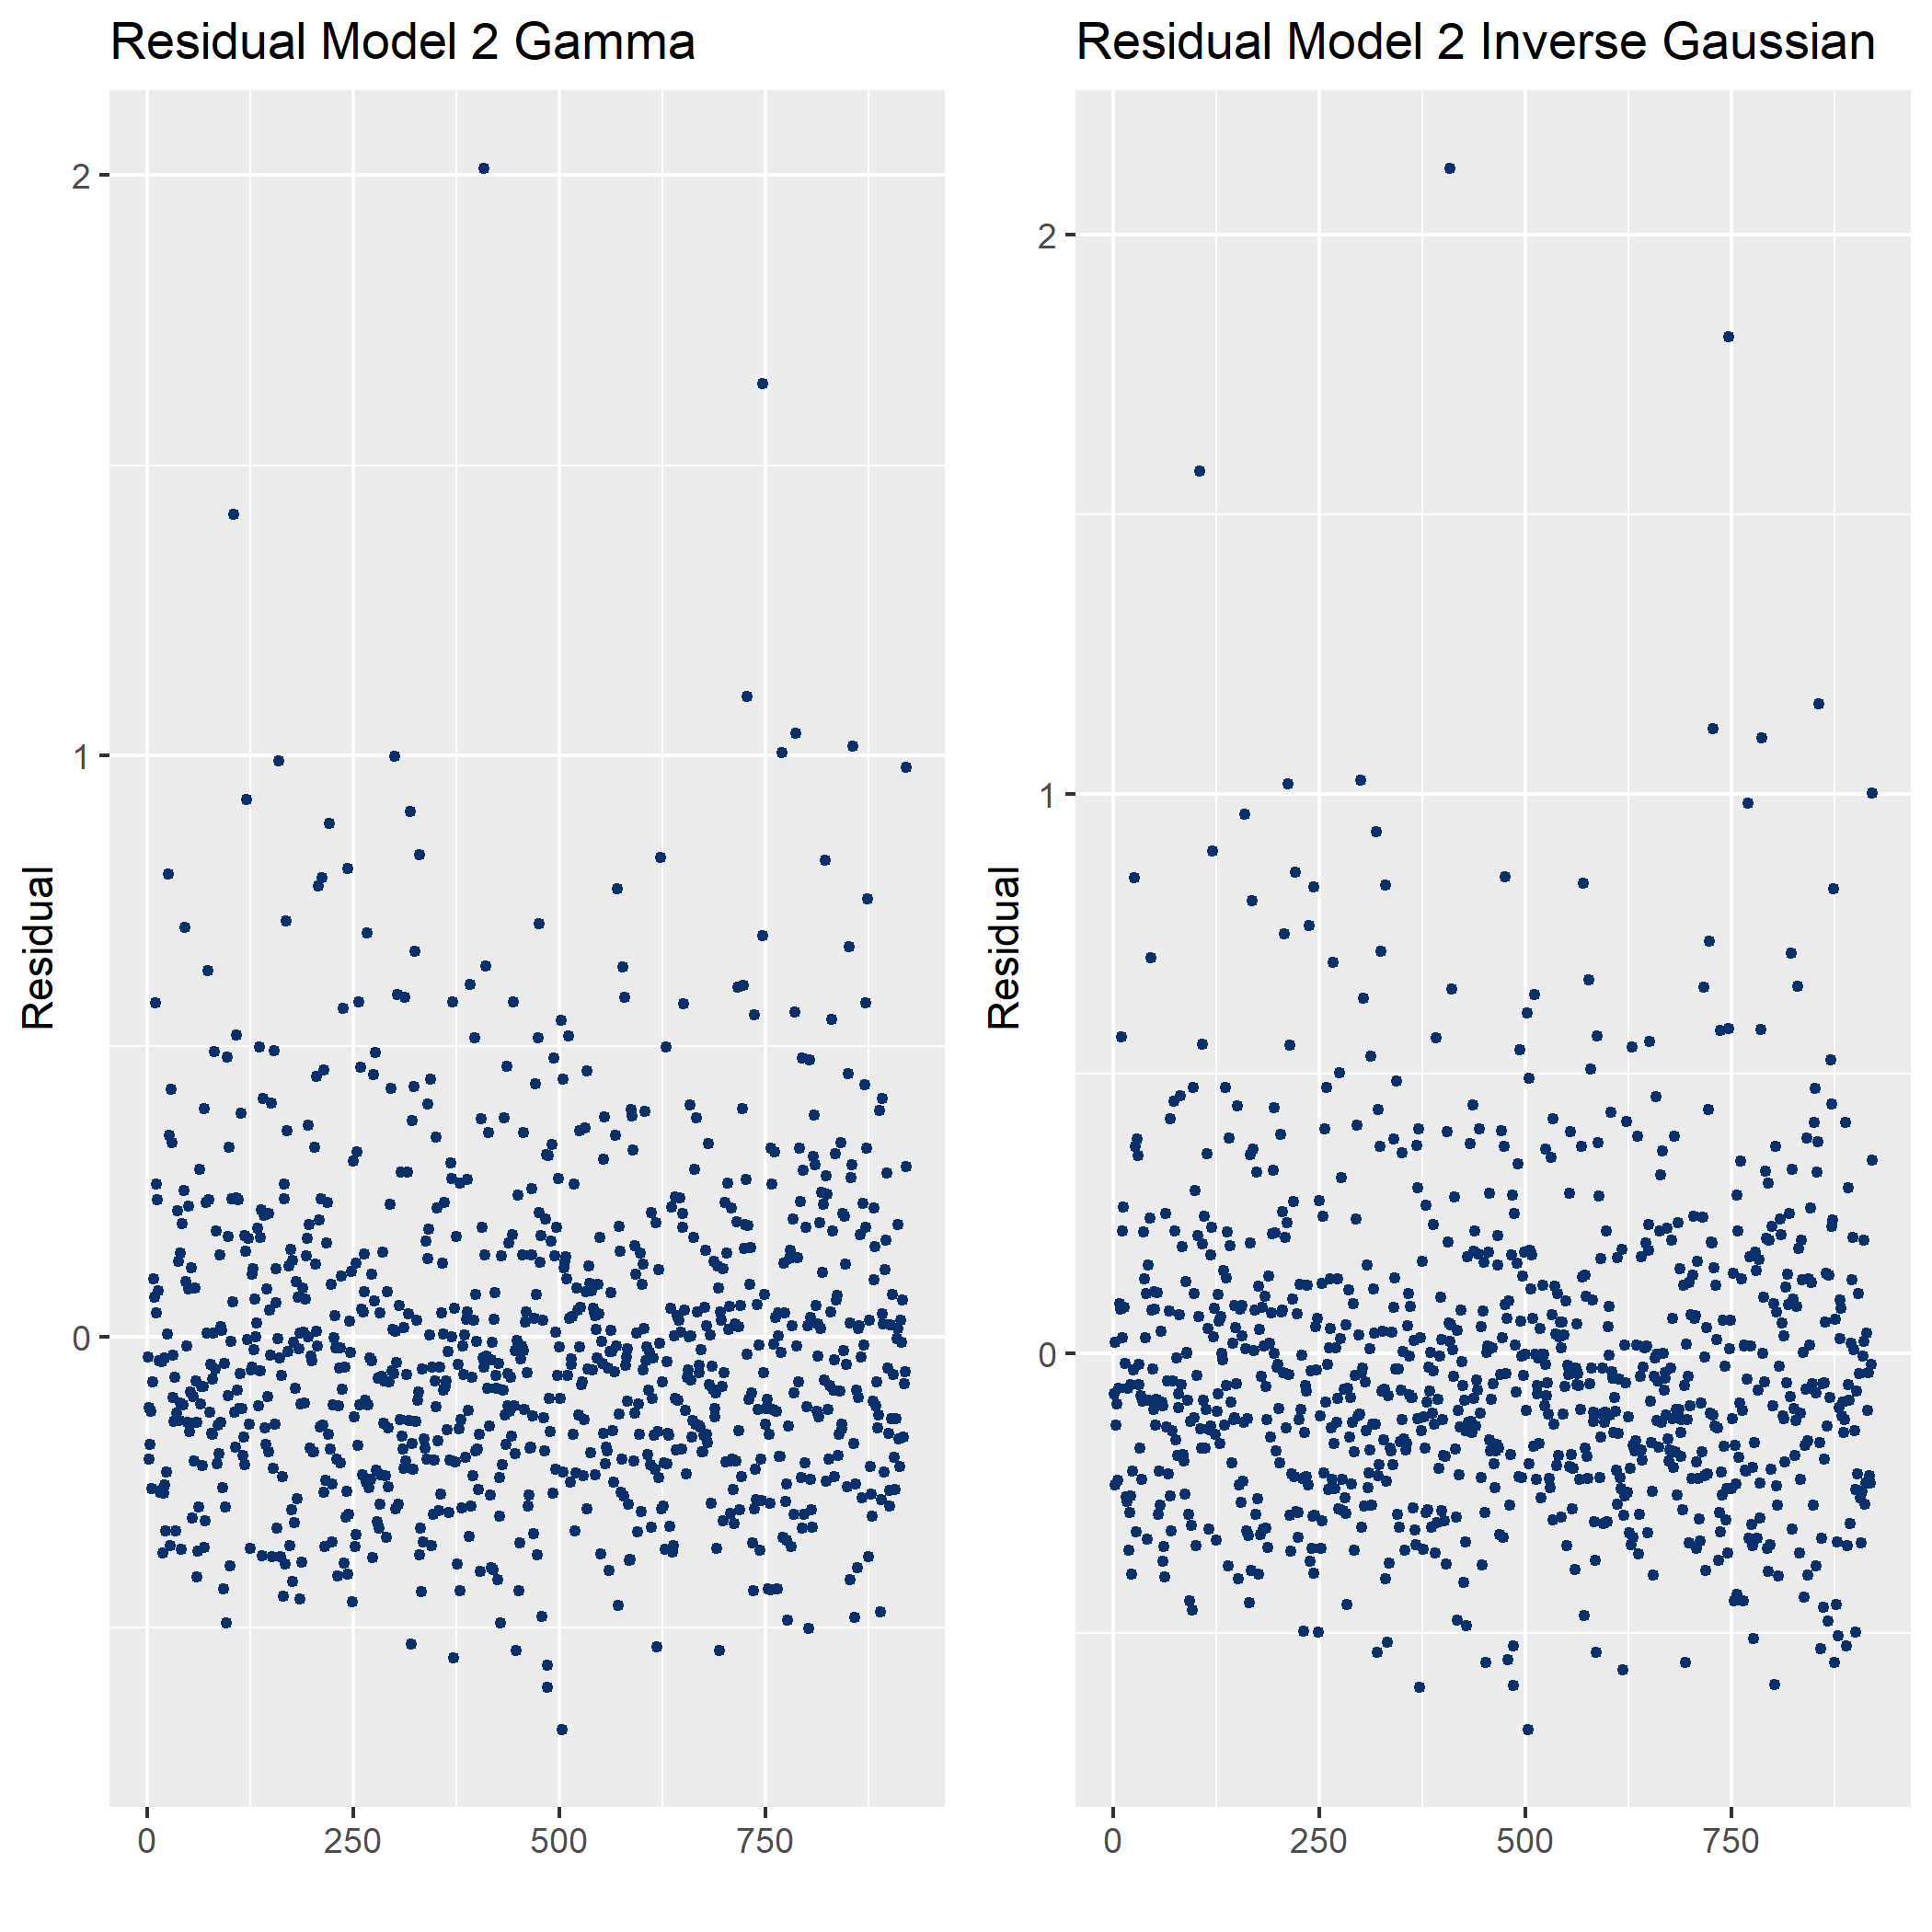
\includegraphics[scale = 0.4]{resid2.png}
    \caption{Residual dari Model Kedua}
    \label{fig:resifddd}
\end{figure}    
\subsection{Contoh Kasus}  
Misalkan ada suatu laptop Dell Ultrabook, 15 inch, ScreenResolution 2560x1600, ScreenType 4K Ultra HD, Cpu\_Series Core i7 8650U, Ram 8GB, Memory\_1\_Type HDD, Memory\_2\_Size 1TB, OpSys Windows 10 maka dengan model pertama dengan distribusi \textit{Inverse Gaussian}, diperoleh nilai rataannya 
\begin{align*}
    \mu_{1,\text{Inv}} &= \exp{(7.03+0.2357-0.03069\times 15+0.1325-0.7158+0.09829+0.03164\times 8} \\
    &-0.1026+0.00005220\times 1024) \\
    &= \exp{6.5243128} = 681.511278
\end{align*}
Misalkan kembali suatu laptop ASUS Gaming ukuran 14 inch dengan ScreenResolution 1366x768, Cpu\_Type Intel, Ram 4GB, Memory\_1\_Type HDD, Gpu\_Type Nvidia, dan OpSys No OS maka dengan model kedua dengan distribusi \textit{Gamma}, diperoleh nilai rataannya 
\begin{align*}
    \mu_{2,\text{Gamma}} &= \exp{(7.1010246-0.1793403+0.0808790-0.0333378\times 14} \\ &-0.2721394 +0.0457834\times4-0.1612674+0.0945031-0.3080577+0.3338656)\\
    &= \exp{6.4058719} = 605.389408
\end{align*}
\newpage
\section{Kesimpulan}
Model yang layak digunakan adalah model dengan distribusi \textit{Gamma} hal ini didukung dari grafik histogram Price\_euros ketika dicocokkan dengan kurva distribusi Gamma bisa dikatakan sangat mendekati distribusi dari Price\_euros. Selain itu  model yang diperoleh memiliki parameter yang signifikan.
\par
Dapat dilihat bahwa performa antara model 1 dan model 2 tidak ada yang dibawah 10\%. Hal ini bisa mengindikasikan bahwa model yang digunakan masih kurang cocok pada data atau data yang ada belum cukup untuk digunakan untuk memodelkan harga laptop karena kombinasi laptop yang beraneka ragam.  
\par
Model pertama khususnya dengan distribusi \textit{Gamma} jauh lebih cocok untuk penjual karena lebih banyak parameter dan juga \textit{error} dari model relatif lebih kecil dibanding model kedua. Sedangkan model kedua jauh lebih cocok untuk pembeli karena parameternya jauh lebih sedikit dan jauh lebih umum dibandingkan model pertama.  
\newpage
\begin{thebibliography}{9}
\bibitem{Buku Cetak SIX}
de Jong, P. dan Heller, G. Z, Generalized Linear Model for Insurance Data, , Cambridge University Press, 2008
\bibitem{Buku Cetak SIX 2}
Walpole, R.E., Myers, R.H., Myers S.L. dan Ye, Keying, Probability and Statistics for Engineers dan Scientists, 9, Prentice‐Hall, 2002

\end{thebibliography}
\newpage
\appendix   
\section{R Code}
\subsection{Package}
\begin{lstlisting}[language=R]
library(readr) # Membaca file .csv
library(dplyr) # Pipeline
library(ggplot2) # Membuat Grafik
library(ggpubr) # Membuat Grafik
library(dgof) # ks.test
library(fitdistrplus) # Menaksir parameter distribusi 
library(actuar) # Menaksir parameter distribusi Inverse Gaussian
library(stringr) # Membersihkan file string
library(SuppDists) # Menaksir parameter distribusi 
library(EnvStats) # Menaksir parameter distribusi 
library(splitstackshape) # Membagi data dengan metode Stratified
\end{lstlisting}
\subsection{Membaca dan Memfilter Data}
\begin{lstlisting}[language=R]
data <- read_csv("laptop_price.csv")
company <- c('Dell','Lenovo','HP','Asus','Acer', 'Apple')
data <- data %>% filter(Company %in% company)
\end{lstlisting}
\subsection{Membersihkan Data}
\subsubsection{Membersihkan Kolom ScreenResolution}
\begin{lstlisting}[language=R]
data$ScreenType <- ''
for (i in 1:nrow(data)){
  vec <- str_split(data$ScreenResolution[i], ' ', simplify = TRUE)
  n <- length(vec)
  if (n > 2){
    m <- n-1
    temp <- vec[1,1]
    for (j in 2:m){
      temp <- paste(temp,vec[1,j])
  }
    data$ScreenType[i] <- temp
    data$ScreenResolution[i] <- vec[1,n]
  }
  else if (n == 2){
    data$ScreenType[i] <- vec[1,1]
    data$ScreenResolution[i] <- vec[1,2]
  }
}
data %>% count(ScreenResolution, sort = T) # Menghitung Jumlah ScreenResolution
data %>% count(ScreenType, sort = T) # Menghitung Jumlah ScreenType
\end{lstlisting}
\subsubsection{Membersihkan Kolom Cpu}
\begin{lstlisting}[language=R]
data$Cpu_Type <- ''
data$Cpu_Series <- ''
data$Cpu_Speed <- ''
for (i in 1:nrow(data)){
  vec <- str_split(data$Cpu[i], ' ',simplify =TRUE)
  n <- length(vec)
  data$Cpu_Type[i] <- vec[1,1]
  data$Cpu_Speed[i] <- vec[1,n]
  n <- n-1
  temp <- vec[1,2]
  for (j in 3:n){
    temp <- paste(temp,vec[1,j])
  }
  data$Cpu_Series[i] <- temp
}
data$Cpu_Speed <- as.numeric(sub('GHz', '', data$Cpu_Speed, fixed=TRUE))
\end{lstlisting}
\subsubsection{Membersihkan Kolom Gpu}
\begin{lstlisting}[language=R]
data$Gpu_Type <- ''
data$Gpu_Series <- ''
for (i in 1:nrow(data)){
  data$Gpu_Type[i] <- str_split(data$Gpu[i], ' ', n=2)[[1]][1]
  data$Gpu_Series[i] <- str_split(data$Gpu[i], ' ', n=2)[[1]][2]
}
\end{lstlisting}
\subsubsection{Membersihkan Kolom Memory}
\begin{lstlisting}[language=R]
data$Memory_1 <- ''
data$Memory_2 <- ''
for (i in 1:nrow(data)){
  data$Memory_1[i] <- sub(' +', '',str_split(data$Memory, ' + ', n=2)[[i]][1],fixed=TRUE)
  data$Memory_2[i] <- str_split(data$Memory, ' + ', n=2)[[i]][2]
}
data$Memory_2[is.na(data$Memory_2)] = 0
data[which(data$Memory_1 =='1.0TB HDD'),]$Memory_1 = '1TB HDD'

data$Memory_1_Type <- ''
data$Memory_1_Size <- ''
data$Memory_2_Type <- ''
data$Memory_2_Size <- ''

for (i in 1:nrow(data)){ 
  data$Memory_1_Type[i] <- str_split(data$Memory_1[i],' ', 2, simplify= T)[1,2]
  data$Memory_1_Size[i] <- str_split(data$Memory_1[i],' ', 2, simplify= T)[1,1]
  
  data$Memory_2_Type[i] <- str_split(data$Memory_2[i],' ', 2, simplify= T)[1,2]
  data$Memory_2_Size[i] <- str_split(data$Memory_2[i],' ', 2, simplify= T)[1,1]
}
data[which(data$Memory_1 =='1.0TB HDD'),]$Memory_1 = '1TB HDD'

data[which(data$Memory_1_Size =='1.0TB'),]$Memory_1_Size = '1TB'
data[which(data$Memory_1_Size =='1TB'),]$Memory_1_Size = '1024GB'
data[which(data$Memory_1_Size =='2TB'),]$Memory_1_Size = '2048GB'

data[which(data$Memory_2_Size =='1.0TB'),]$Memory_2_Size = '1TB'
data[which(data$Memory_2_Size =='1TB'),]$Memory_2_Size = '1024GB'
data[which(data$Memory_2_Size =='2TB'),]$Memory_2_Size = '2048GB'

data$Memory_1_Size <- sub('GB', "", data$Memory_1_Size,fixed = TRUE)
data$Memory_1_Size <- as.numeric(data$Memory_1_Size)
data$Memory_2_Size <- sub('GB', "", data$Memory_2_Size,fixed = TRUE)
data$Memory_2_Size <- as.numeric(data$Memory_2_Size)
\end{lstlisting}
\subsubsection{Membersihkan Kolom Ram}
\begin{lstlisting}[language=R]
data$Ram <- as.numeric(sub('GB', "", data$Ram,fixed = TRUE))
\end{lstlisting}
\subsubsection{Membersihkan Kolom Weight}
\begin{lstlisting}[language=R]
data$Weight <-as.numeric(str_remove(data$Weight,'kg'))
\end{lstlisting}
\subsection{Mengolah Data}
\subsubsection{Menyesuaikan Tipe Kolom dan Me-\textit{relevel} Ulang}
\begin{lstlisting}[language=R]
data$Company <- relevel(factor(data$Company), 'Dell')
data$Product <- relevel(factor(data$Product), 'XPS 13')
data$TypeName <- relevel(factor(data$TypeName), 'Notebook')
data$ScreenResolution <- relevel(factor(data$ScreenResolution), '1920x1080')
data$ScreenType <- relevel(factor(data$ScreenType), 'Full HD')
data$Cpu_Type <- relevel(factor(data$Cpu_Type), 'Intel')
data$Cpu_Series <- relevel(factor(data$Cpu_Series), 'Core i5 7200U')
data$Memory_1_Type <- relevel(factor(data$Memory_1_Type), 'SSD')
data$Memory_2_Type <- relevel(factor(data$Memory_2_Type), '')
data$Gpu_Type <- factor(data$Gpu_Type)
data$Gpu_Series <- factor(data$Gpu_Series)
data$OpSys <- relevel(factor(data$OpSys), 'Windows 10')
\end{lstlisting}
\subsection{Memodelkan Data}
\subsubsection{Menentukan Distribusi yang Cocok}
\begin{lstlisting}[language=R]
set.seed(10818015)

summary(fitdist(data$Price_euros,"gamma"))

ks.test(data$Price_euros,rgamma(nrow(data),
shape = 2.928053153,rate = 0.002717365),
alternative = "two.sided",exact = TRUE)

summary(fitdist(data$Price_euros,"invgauss",
method='mle',lower=c(0,0)
,start = list(mean = mean(data$Price_euros), 
shape = sd(data$Price_euros))))

ks.test(data$Price_euros,rinvgauss(nrow(data),
mean = 1077.554,shape = 2433.434),
alternative = "two.sided",exact = TRUE)
\end{lstlisting}

\subsubsection{Membagi Data Menjadi \textit{Train} dan \textit{Test}}
\begin{lstlisting}[language=R]
set.seed(10818015)
temp <- stratified(data, group =25, size = 0.8, bothSets = T)
train <- as.data.frame(temp$SAMP1)
test <- as.data.frame(temp$SAMP2)
\end{lstlisting}

\subsubsection{Membangun dan Memeriksa Signifikansi Model}
\begin{lstlisting}[language=R]
set.seed(10818015)
model1 <- step(glm(Price_euros ~ Company + TypeName + Inches +
                  ScreenResolution + ScreenType + Cpu_Series+ Cpu_Type +
                  Cpu_Speed + Ram + Memory_1_Type + Memory_1_Size +
                  Memory_2_Type + Memory_2_Size + Gpu_Series+Gpu_Type+
                  OpSys,
                family = Gamma(link ="log"),
                data=train),direction ="both",trace = F)
summary(model1)
anova(model1,test="Chisq")
confint(model1)
y_hat <- exp(predict(model1,train$Price_euros))
mape(train$Price_euros,y_hat)

model1inv <- step(glm(Price_euros ~ Company + TypeName + Inches +
                  ScreenResolution + ScreenType + Cpu_Series+ Cpu_Type +
                  Cpu_Speed + Ram + Memory_1_Type + Memory_1_Size +
                  Memory_2_Type + Memory_2_Size + Gpu_Series+Gpu_Type+
                  OpSys,
                family = inverse.gaussian(link ="log"),
                data=train),direction ="both",trace = F)
summary(model1inv)
anova(model1inv, test="Chisq")
confint(model1inv)

y_hat <- exp(predict(model1inv, train$Price_euros))
mape(train$Price_euros,y_hat)

model2 <- step(glm(Price_euros ~
Company + TypeName + Inches+ ScreenResolution
+ Cpu_Type + Ram+ Memory_1_Size+
                   Memory_1_Type+Gpu_Type+ OpSys+Company*OpSys+Company*TypeName ,
                 family = Gamma(link ="log"),
                data=train),direction ="both",trace = F)
summary(model2)
anova(model2,test="Chisq")
confint(model2)
y_hat <- exp(predict(model2, train$Price_euros))
mape(train$Price_euros,y_hat)
y_hat <- exp(predict(model2, test$Price_euros))
mape(test$Price_euros,y_hat)

model2inv <- step(glm(Price_euros ~
Company + TypeName + Inches
+ ScreenResolution + Cpu_Type +
Ram+Memory_1_Size+
                   Memory_1_Type+Gpu_Type+ OpSys+Company*OpSys+Company*TypeName ,
                 family = inverse.gaussian(link ="log"),
                data=train),direction ="both",trace = F)
summary(model2inv)
anova(model2inv,test="Chisq")
confint(model2inv)
y_hat <- exp(predict(model2inv, train$Price_euros))
mape(train$Price_euros,y_hat)
y_hat <- exp(predict(model2inv, test$Price_euros))
mape(test$Price_euros,y_hat)
\end{lstlisting}

\subsubsection{Membangun DataFrame Residual}
\begin{lstlisting}[language=R]
set.seed(10818015)
residual <- data.frame(1:nrow(train),model1$residuals, model1inv$residuals, 
model2$residuals, model2inv$residuals)
\end{lstlisting}

\subsection{Kode untuk Grafik}
\begin{lstlisting}[language=R]

data %>%
 filter(!(Memory_2_Type %in% "")) %>%
 ggplot() +
 aes(x = Company, fill = TypeName) +
 geom_bar() +
 scale_fill_hue() +
 labs(y = "Frekuensi", title = "Banyak Laptop Berdasarkan Company dan TypeName") +
 theme_gray()

ggplot(data1) +
 aes(x = "", y = Inches, fill = Company) +
 geom_boxplot() +
 scale_fill_brewer(palette = "BrBG") +
 labs(x = "Data yang Sudah Difilter", y = "Inches", title = "Box Plot dari Masing-Masing Company") +
 theme_gray()

ggplot(data1) +
 aes(x = "", y = Inches, fill = Company) +
 geom_boxplot() +
 scale_fill_brewer(palette = "BrBG") +
 labs(x = "Data yang Sudah Difilter", y = "Inches", title = "Box Plot dari Masing-Masing Company") +
 theme_gray()
 
ggplot(data) +
 aes(x = OpSys) +
 geom_bar(fill = "#6baed6") +
 labs(y = "Frekuensi", title = "Banyak Laptop Berdasarkan OpSys") +
 theme_gray()

ggplot(data) +
 aes(x = TypeName) +
 geom_bar(fill = "#6baed6") +
 labs(y = "Frekuensi", title = "Banyak Laptop Berdasarkan Tipe") +
 theme_gray()

ggplot(data) +
 aes(x = Company) +
 geom_bar(fill = "#6baed6") +
 labs(y = "Frekuensi", title = "Banyak Laptop Berdasarkan Perusahaan") +
 theme_gray()

ggplot(data) +
 aes(x = Price_euros) +
 geom_histogram(bins = 30L, fill = "#6baed6") +
 labs(y = "Frekuensi", title = "Distribusi Harga Laptop") +
 theme_gray()

ggsave('barplot_inter1.png')
data %>%
 filter(!(ScreenType %in% "")) %>%
 ggplot() +
 aes(x = "", y = Price_euros, fill = ScreenType) +
 geom_boxplot() +
labs(x = "ScreenResolution", title = "Boxplot Harga Laptop Berdasarkan ScreenResolution")+
 scale_fill_hue() +
 theme_gray()

dp <-ggplot(data) +
 aes(x = "", y = Price_euros, fill = Gpu_Type) +
 geom_boxplot() +
 scale_fill_hue() +
 labs(x = "Gpu_Type", title = "Box Plot Harga Berdasarkan Gpu_Type") +
 theme_gray()

bxp <- ggplot(data) +
 aes(x = "", y = Price_euros, fill = Cpu_Type) +
 geom_boxplot() +
 scale_fill_hue() +
 labs(x = "Cpu_Type", title = "Box Plot Harga Berdasarkan Cpu_Type") +
 theme_gray()

dp <- data %>%
 filter(!(ScreenType %in% "")) %>%
 ggplot() +
 aes(x = "", y = Price_euros, fill = Gpu_Type) +
 geom_boxplot() +
 scale_fill_hue() +
 labs(x = "ScreenType", title = "Boxplot Harga Laptop Berdasarkan ScreenType") +
 theme_gray()

ggarrange(bxp, dp, ncol = 2, nrow = 1)
ggsave('boxplot_price3.png')

bxp <- data %>%
 filter(!(ScreenType %in% "")) %>%
 filter(!(Memory_2_Type %in% "")) %>%
 ggplot() +
 aes(x = Memory_1_Size, y = Price_euros) +
 geom_point(size = 1L, colour = "#6baed6") +
 labs(title = "Diagram Pencar antara Harga Laptop dengan Memory_1_Size") +
 theme_gray()

dp <- data %>%
 filter(!(ScreenType %in% "")) %>%
 filter(!(Memory_2_Type %in% "")) %>%
 ggplot() +
 aes(x = Memory_2_Size, y = Price_euros) +
 geom_point(size = 1L, colour = "#6baed6") +
 labs(title = "Diagram Pencar antara Harga Laptop dengan Memory_2_Size") +
 theme_gray()
ggarrange(bxp, dp, ncol = 2, nrow = 1)
ggsave('scatter_price0.png',limitsize = F)

ggplot(data) +
 aes(x = Company, fill = OpSys) +
 geom_bar() +
 scale_fill_hue() +
 labs(y = "Frekuensi", title = "Banyak Laptop Berdasarkan Company dan OpSys") +
 theme_gray()

data %>%
 filter(!(ScreenType %in% "")) %>%
 filter(!(Memory_2_Type %in% "")) %>%
 ggplot() +
 aes(x = Inches, y = Weight) +
 geom_point(size = 1L, colour = "#0c4c8a") +
 labs(title = "Korelasi Antara Weight dengan Inches") +
 theme_gray()
ggsave('inchesweight.png')

x<-ggplot(residual) +
 aes(x = X1.nrow.train., y = model1.residuals) +
 geom_point(size = 1L, colour = "#08306b") +
 labs(x = "  ", y = "Residual", title = "Residual Model 1 Gamma") +
 theme_gray()

y<-ggplot(residual) +
 aes(x = X1.nrow.train., y = model1inv.residuals) +
 geom_point(size = 1L, colour = "#08306b") +
 labs(x = "  ", y = "Residual", title = "Residual Model 1 Inverse Gaussian") +
 theme_gray()

x <-ggplot(residual) +
 aes(x = X1.nrow.train., y = model2inv.residuals) +
 geom_point(size = 1L, colour = "#08306b") +
 labs(x = "  ", y = "Residual", title = "Residual Model 2 Inverse Gaussian") +
 theme_gray()

y<- ggplot(residual) +
 aes(x = X1.nrow.train., y = model2.residuals) +
 geom_point(size = 1L, colour = "#08306b") +
 labs(x = "  ", y = "Residual", title = "Residual Model 2 Gamma") +
 theme_gray()
ggarrange(x,y,nrow=1,ncol=2)
ggsave('resid1.png')
\end{lstlisting}
\newpage
\section{Hasil Output Model dan Selang Kepercayaan}
\subsection{Model 1 \textit{Gamma}}
\label{Model_1_Gamma}
\begin{figure}[h!]
    \centering
    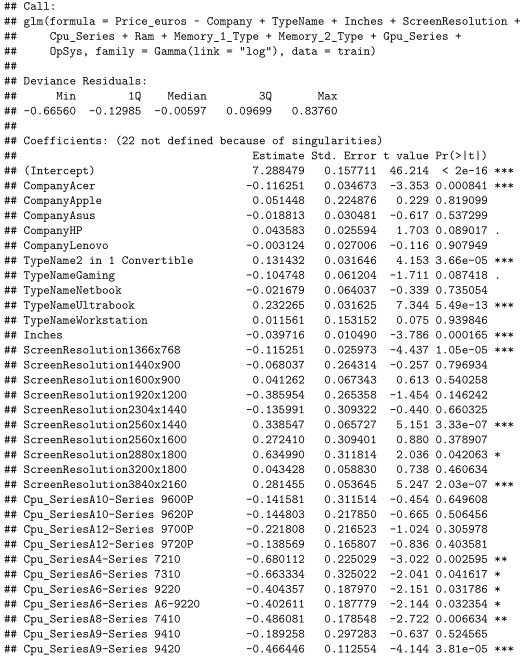
\includegraphics{Model_1_Sum(1_3).png}
    \label{fig:SUM11}
\end{figure}
\begin{figure}[h!]
    \centering
    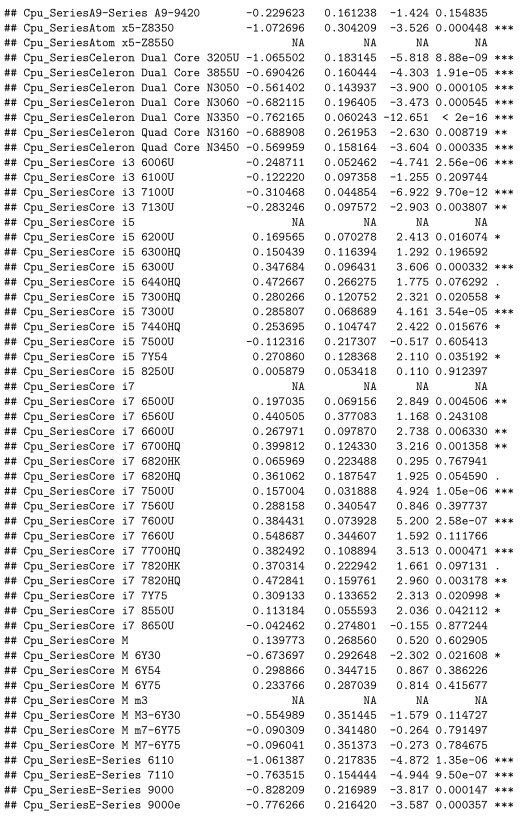
\includegraphics{Model_1_Sum(2_3).png}
    \label{fig:SUM12}
\end{figure}
\begin{figure}[h!]
    \centering
    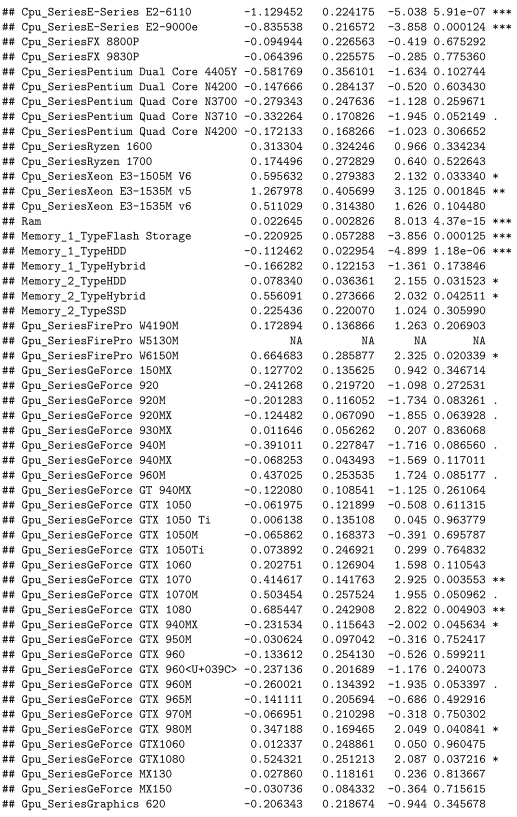
\includegraphics{Model_1_Sum(3_3).png}
    \label{fig:SUM13}
\end{figure}
\begin{figure}[h!]
    \centering
    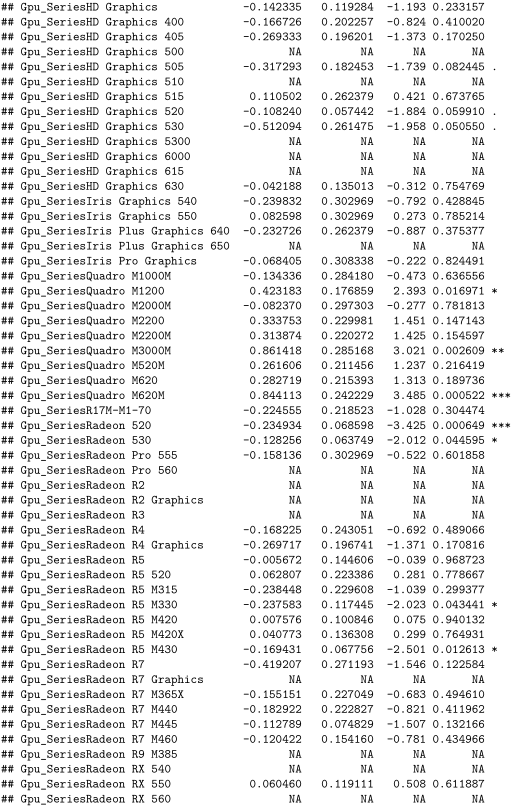
\includegraphics{Model_1_Sum(4_3).png}
    \label{fig:SUM14}
\end{figure}
\begin{figure}[h!]
    \centering
    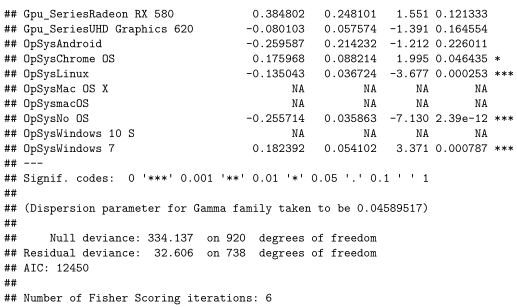
\includegraphics{Model_1_Sum(5_3).png}
    \caption{Hasil Luaran Parameter Model 1 \textit{Gamma}}
    \label{fig:SUM15}
\end{figure}
\begin{figure}[h!]
    \centering
    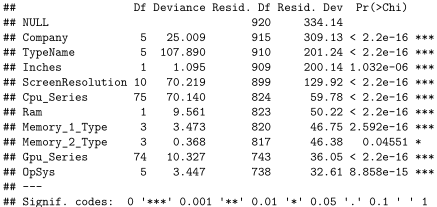
\includegraphics{Model_1_AOV.png}
    \caption{Hasil Luaran Analysis of Deviance Model 1 \textit{Gamma}}
    \label{fig:AOV}
\end{figure}
\begin{figure}[h!]
    \centering
    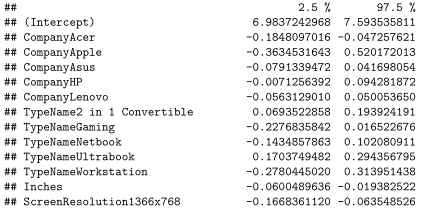
\includegraphics{Model_1_CI(1_5).png}
    \label{fig:CI11}
\end{figure}
\begin{figure}[h!]
    \centering
    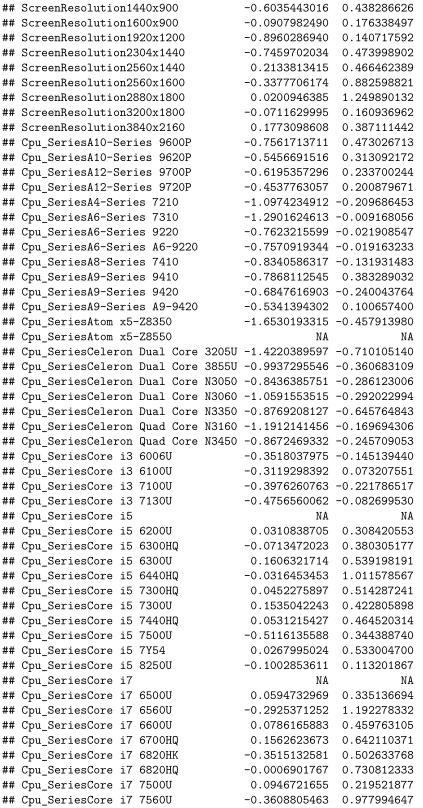
\includegraphics{Model_1_CI(2_5).png}
    \label{fig:CI12}
\end{figure}
\begin{figure}[h!]
    \centering
    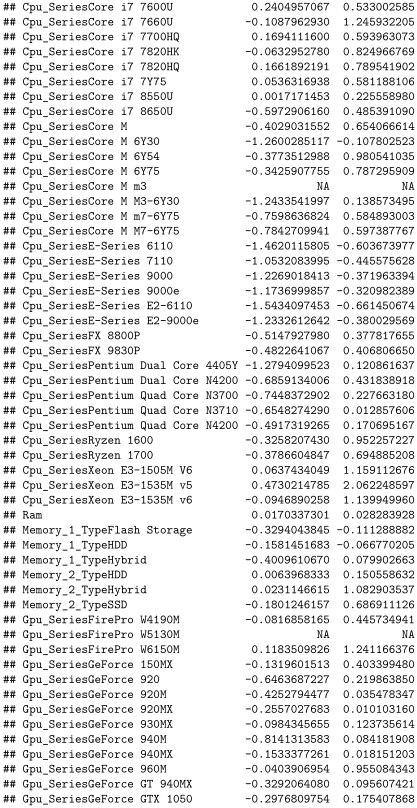
\includegraphics{Model_1_CI(3_5).png}
    \label{fig:CI13}
\end{figure}
\begin{figure}[h!]
    \centering
    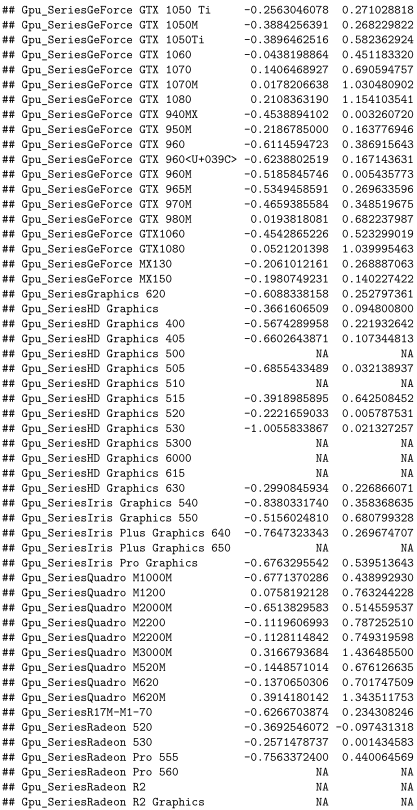
\includegraphics{Model_1_CI(4_5).png}
    \label{fig:CI14}
\end{figure}
\begin{figure}[h!]
    \centering
    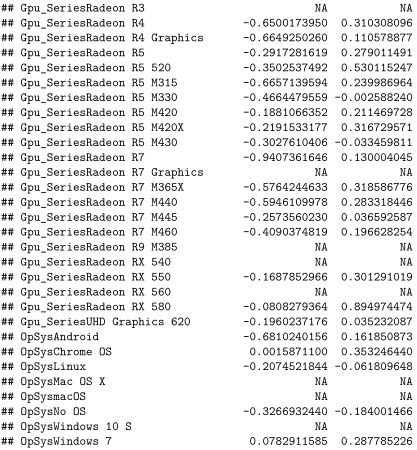
\includegraphics{Model_1_CI(5_5).png}
    \caption{Hasil Luaran Selang Kepercayaan Parameter Model 1 \textit{Gamma}}
    \label{fig:CI15}
\end{figure}
\subsection{Model 1 \textit{Inverse Gaussian}}
\label{Model_1_Inv}
\begin{figure}[h!]
    \centering
    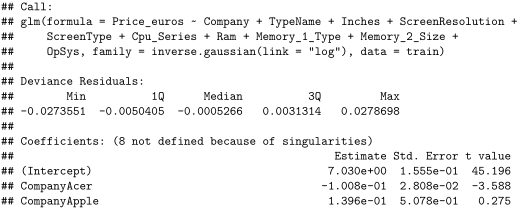
\includegraphics{Model_2_Sum(1_3).png}
    \label{fig:SUM21}
\end{figure}
\begin{figure}[h!]
    \centering
    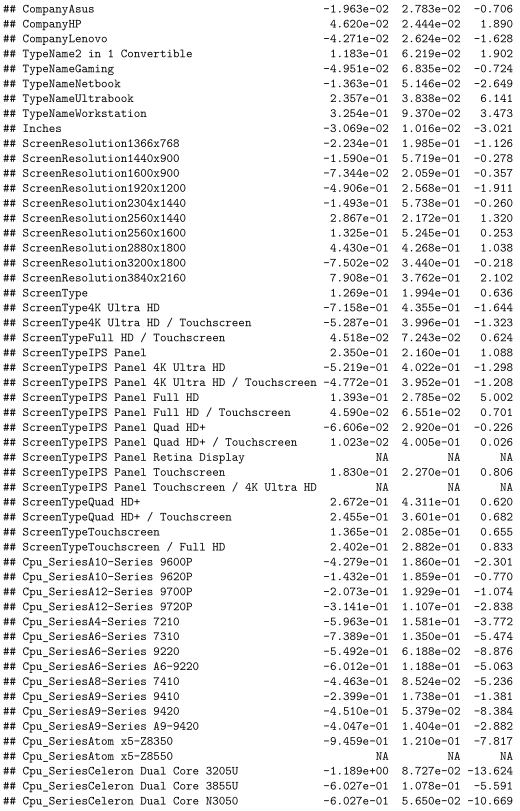
\includegraphics{Model_2_Sum(2_3).png}
    \label{fig:SUM22}
\end{figure}
\begin{figure}[h!]
    \centering
    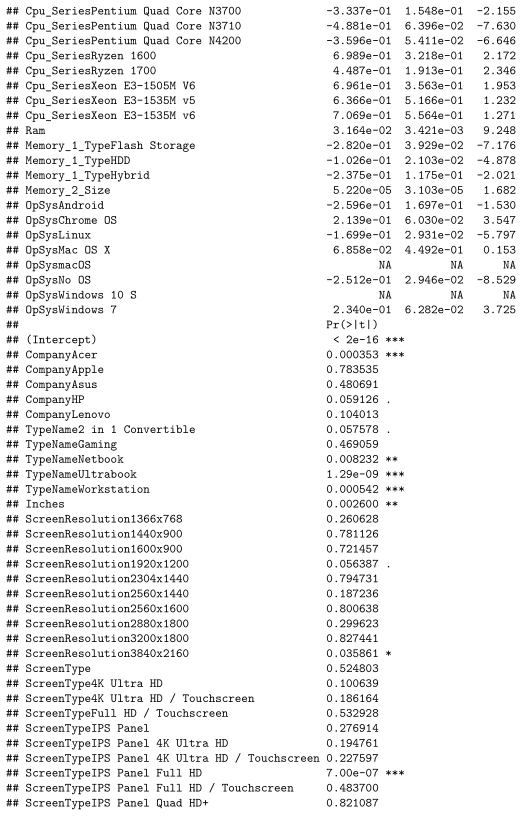
\includegraphics{Model_2_Sum(3_3).png}
    \label{fig:SUM23}
\end{figure}
\begin{figure}[h!]
    \centering
    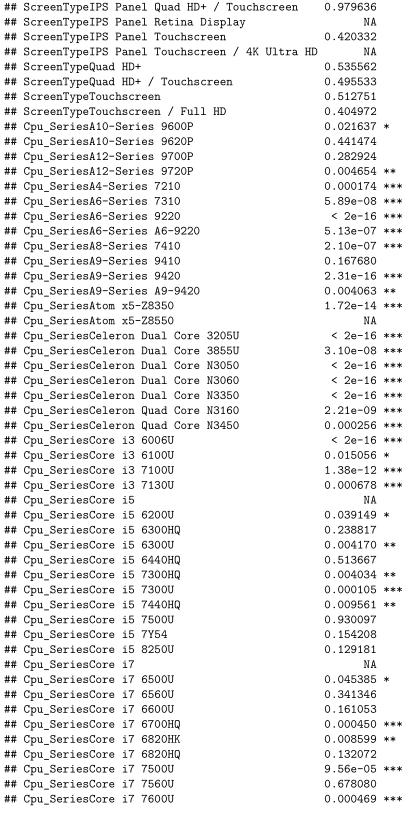
\includegraphics{Model_2_Sum(4_3).png}
    \label{fig:SUM24}
\end{figure}
\begin{figure}[h!]
    \centering
    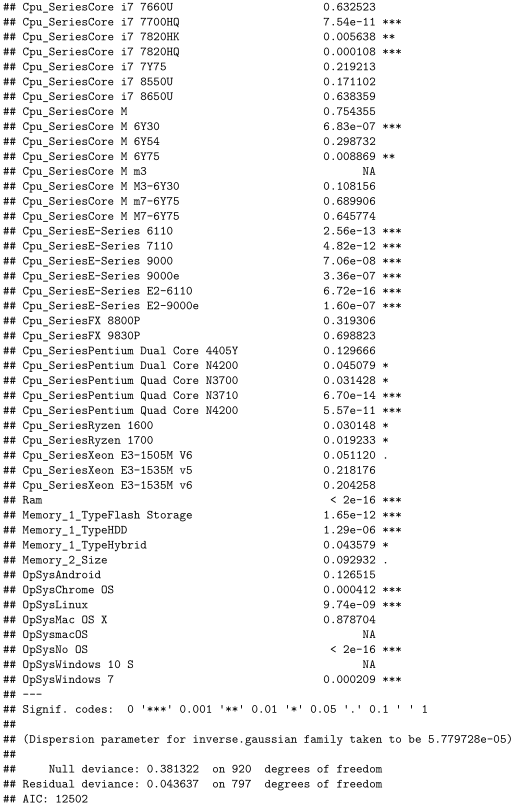
\includegraphics{Model_2_Sum(5_3).png}
    \label{fig:SUM25}
\end{figure}
\begin{figure}[h!]
    \centering
    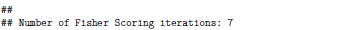
\includegraphics{Model_2_Sum(6_3).png}
    \caption{Hasil Luaran Parameter Model 1 \textit{Inverse Gaussian}}
    \label{fig:SUM26}
\end{figure}
\begin{figure}[h!]
    \centering
    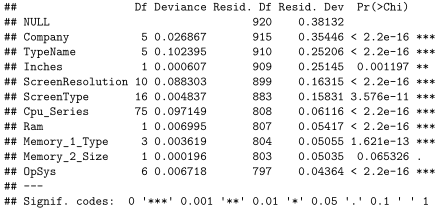
\includegraphics{Model_2_AOV.png}
    \caption{Hasil Luaran Analysis of Deviance Model 1 \textit{Inverse Gaussian}}
    \label{fig:AOV2}
\end{figure}
\begin{figure}[h!]
    \centering
    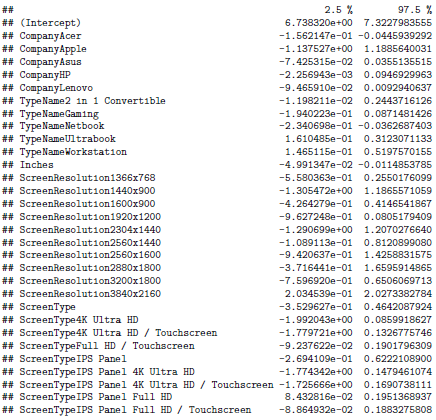
\includegraphics{Model_2_CI(1_5).png}
    \label{fig:CI21}
\end{figure}
\begin{figure}[h!]
    \centering
    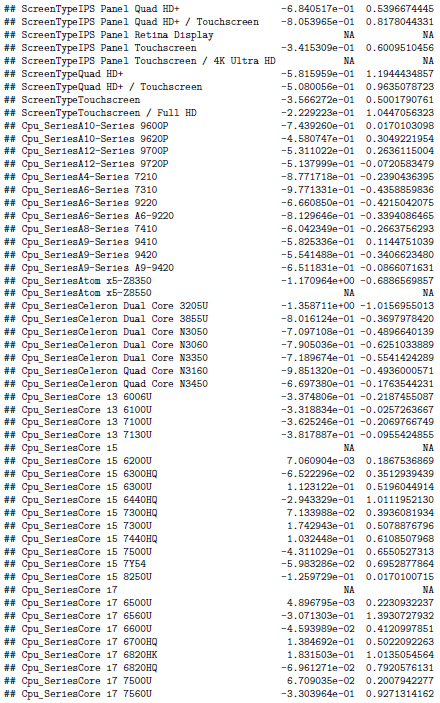
\includegraphics{Model_2_CI(2_5).png}
    \label{fig:CI22}
\end{figure}
\begin{figure}[h!]
    \centering
    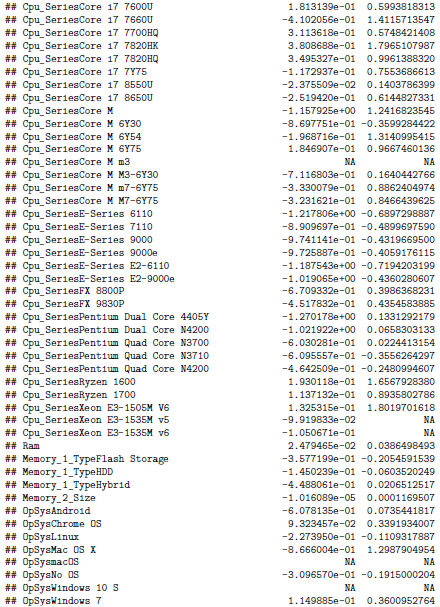
\includegraphics{Model_2_CI(3_5).png}
    \caption{Hasil Luaran Selang Kepercayaan Parameter Model 1 \textit{Inverse Gaussian}}
    \label{fig:CI23}
\end{figure}
\subsection{Model 2 \textit{Gamma}}
\label{Model_2_Gamma}
\begin{figure}[h!]
    \centering
    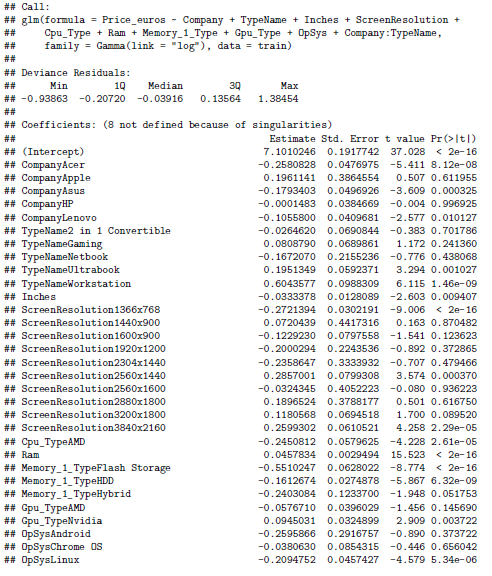
\includegraphics{Model_3_Sum(1_3).png}
    \label{fig:SUM31}
\end{figure}
\begin{figure}[h!]
    \centering
    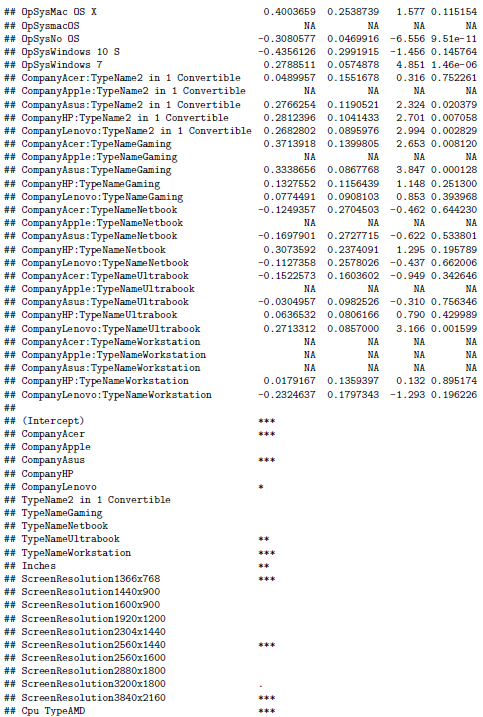
\includegraphics{Model_3_Sum(2_3).png}
    \label{fig:SUM32}
\end{figure}
\begin{figure}[h!]
    \centering
    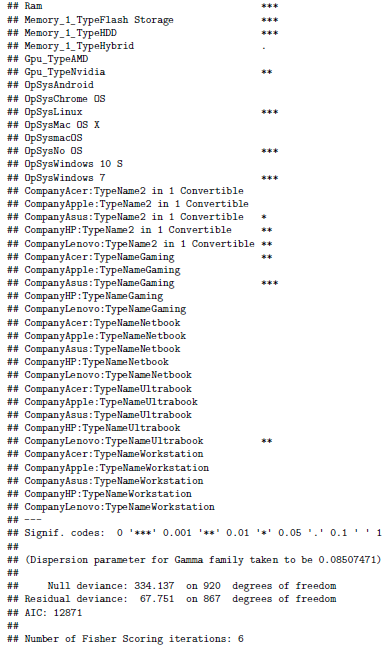
\includegraphics{Model_3_Sum(3_3).png}
    \caption{Hasil Luaran Parameter Model 2 \textit{Gamma}}
    \label{fig:SUM33}
\end{figure}
\begin{figure}[h!]
    \centering
    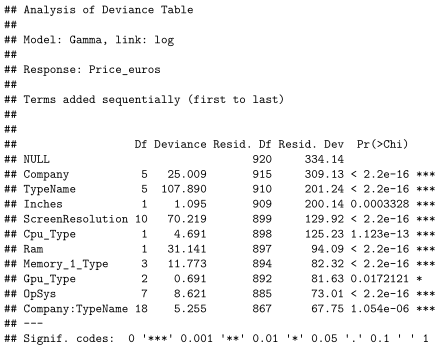
\includegraphics{Model_3_AOV.png}
    \label{fig:AOV3}
    \caption{Hasil Luaran Analysis of Deviance Model 2 \textit{Gamma}}
\end{figure}
\begin{figure}[h!]
    \centering
    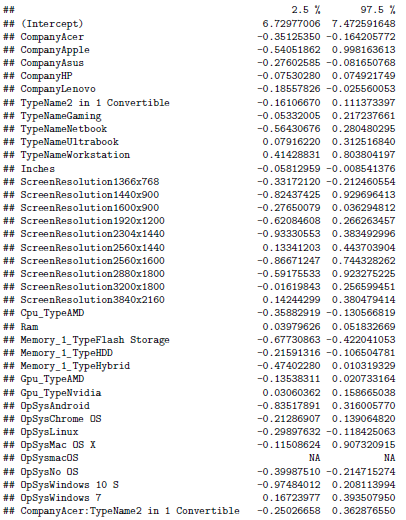
\includegraphics{Model_3_CI(1_5).png}
    \label{fig:CI31}
\end{figure}
\begin{figure}[h!]
    \centering
    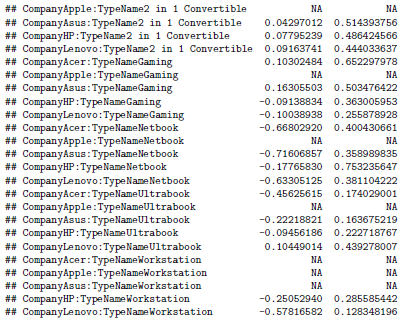
\includegraphics{Model_3_CI(2_5).png}
    \caption{Hasil Luaran Selang Kepercayaan Parameter Model 2 \textit{Gamma}}
    \label{fig:CI32}
\end{figure}
\subsection{Model 2 \textit{Inverse Gaussian}}
\label{Model_2_Inv}
\begin{figure}[h!]
    \centering
    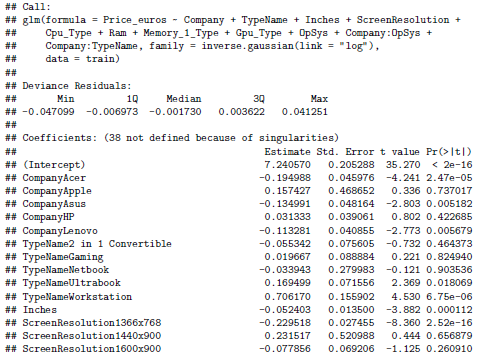
\includegraphics{Model_4_Sum(1_3).png}
    \label{fig:sum41}
\end{figure}
\begin{figure}[h!]
    \centering
    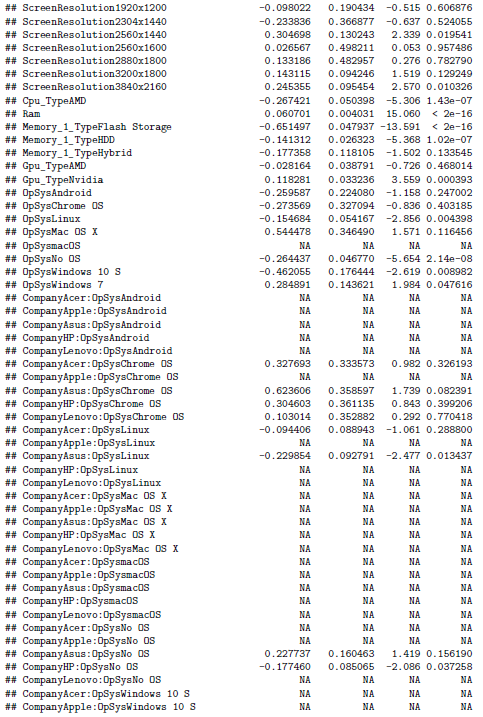
\includegraphics{Model_4_Sum(2_3).png}
    \label{fig:sum42}
\end{figure}
\begin{figure}[h!]
    \centering
    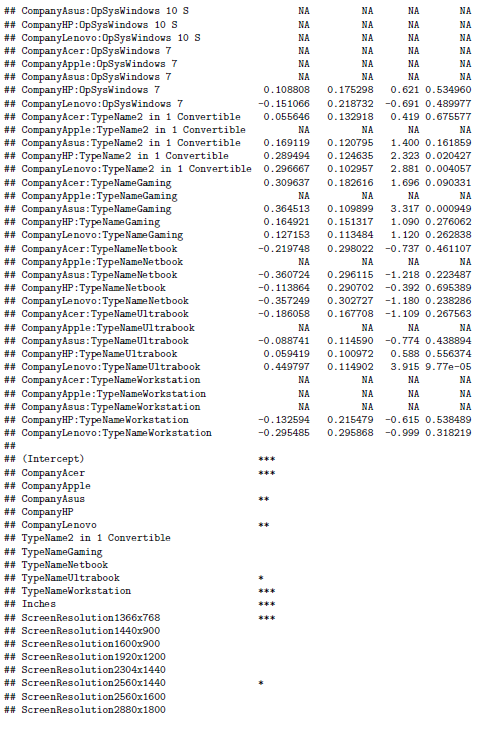
\includegraphics{Model_4_Sum(3_3).png}
    \label{fig:sum43}
\end{figure}
\begin{figure}[h!]
    \centering
    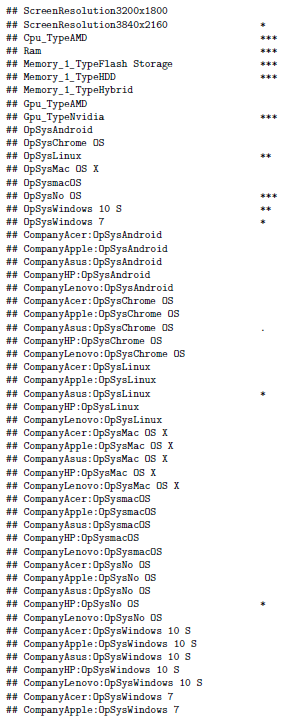
\includegraphics{Model_4_Sum(4_3).png}
    \label{fig:sum44}
\end{figure}
\begin{figure}[h!]
    \centering
    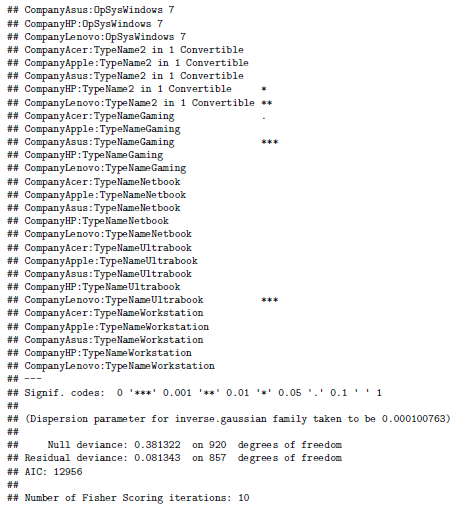
\includegraphics{Model_4_Sum(5_3).png}
    \caption{Hasil Luaran Parameter Model 2 \textit{Inverse Gaussian}}
    \label{fig:sum45}
\end{figure}
\begin{figure}[h!]
    \centering
    \includegraphics{Model_4_AOV.png}
    \caption{Hasil Luaran Analysis of Deviance Model 2 \textit{Inverse Gaussian}}
    \label{fig:AOV4}
\end{figure}
\begin{figure}[h!]
    \centering
    \includegraphics{Model_4_CI(1_5).png}
    \label{fig:CI41}
\end{figure}
\begin{figure}[h!]
    \centering
    \includegraphics{Model_4_CI(2_5).png}
    \caption{Hasil Luaran Selang Kepercayaan Parameter Model 2 \textit{Inverse Gaussian}}
    \label{fig:CI42}
\end{figure}
\end{document}
